\chapter{High Voltage System}
\label{ch:fdsp-hv}

%%%%%%%%%%%%%%%%%%%%%%%%%%%%%%%%%%%%%%%%%%%%%%%%%%%%%%%%%%%%%%%%%%%%
\section{High Voltage System Overview}
\label{sec:fdsp-hv-ov}


%%%%%%%%%%%%%%%%%%%%%%%%%%%%%%%%%
\subsection{Introduction}
\label{sec:fdsp-hv-intro}

A \dword{lartpc} requires an equipotential cathode plane at \dword{hv} and a precisely regulated interior \efield{} to drive 
electrons from particle interactions to sensor planes.  In the case of the DUNE \dlong{sp} technology, 
this requires vertical cathode planes, called \dwords{cpa}, held at \dword{hv}; vertical anode planes, called \dwords{apa}, described in Chapter~\ref{sec:fdsp-apa-intro}; and formed sets of conductors at graded voltages surrounding the
 the central drift volume, collectively called the \dlong{fc}. The \dword{fc} consists of portions on the top and bottom  
of the drift volume (called the \dword{topfc} and \dword{botfc}, respectively), and along the sides, called \dwords{ewfc}.

\fixme{\dword{cpa} by itself is the only form of \dword{cpa} not defined. What is the cathode plane ``assembly'' as opposed to the \dword{cpa} plane, panel, array, unit...? RKP: Believe this is clear as written.}

The SP \dword{tpc} construction is shown in Figure~\ref{fig:dune_sp_fd}.
%A DUNE \dword{spmod} is made up of 4 drif, plus two complete  \dword{ewfc} planes, with 
The  drift fields transport the ionization electrons 
%in the direction \dword{cpa} $\Rightarrow$ \dword{apa}. 
towards the \dwords{apa} at sides and center.
One should note that the \dword{hv} systems for the \single and \dual TPC concepts share components with similar designs. These include the \dwords{fc} profiles and supporting FRP beams as well as the voltage divider boards. More details can be found in \voltitledpfd Chapter 4.


\begin{dunefigure}[One unit of the \dword{spmod}]% showing \dwords{cpa} and \dwords{apa}]
{fig:dune_sp_fd}
{%Interior of a \dword{spmod}. The \dwords{cpa} occupy the second and fourth positions, between the three \dwords{apa}.  \Dwords{topfc} and \dwords{botfc} field cages are shown in blue (Image: CAD model).
A schematic of a \dword{spmod} showing the three \dword{apa} arrays (at the far left and right and in the center, spanning the entire \dword{detmodule} length) and the two \dword{cpa} arrays, occupying the intermediate second and fourth positions. The top and bottom \dword{fc} modules are shown in blue; the \dwords{ewfc} are not shown. 
On the right, the front top and bottom \dword{fc} modules are shown folded up against the \dword{cpa} panels to which they connect, as they are positioned for shipping and insertion into the cryostat.  The \dwords{cpa}, \dwords{apa} and \dwords{fc} together define the four drift volumes of the \dword{spmod}.}
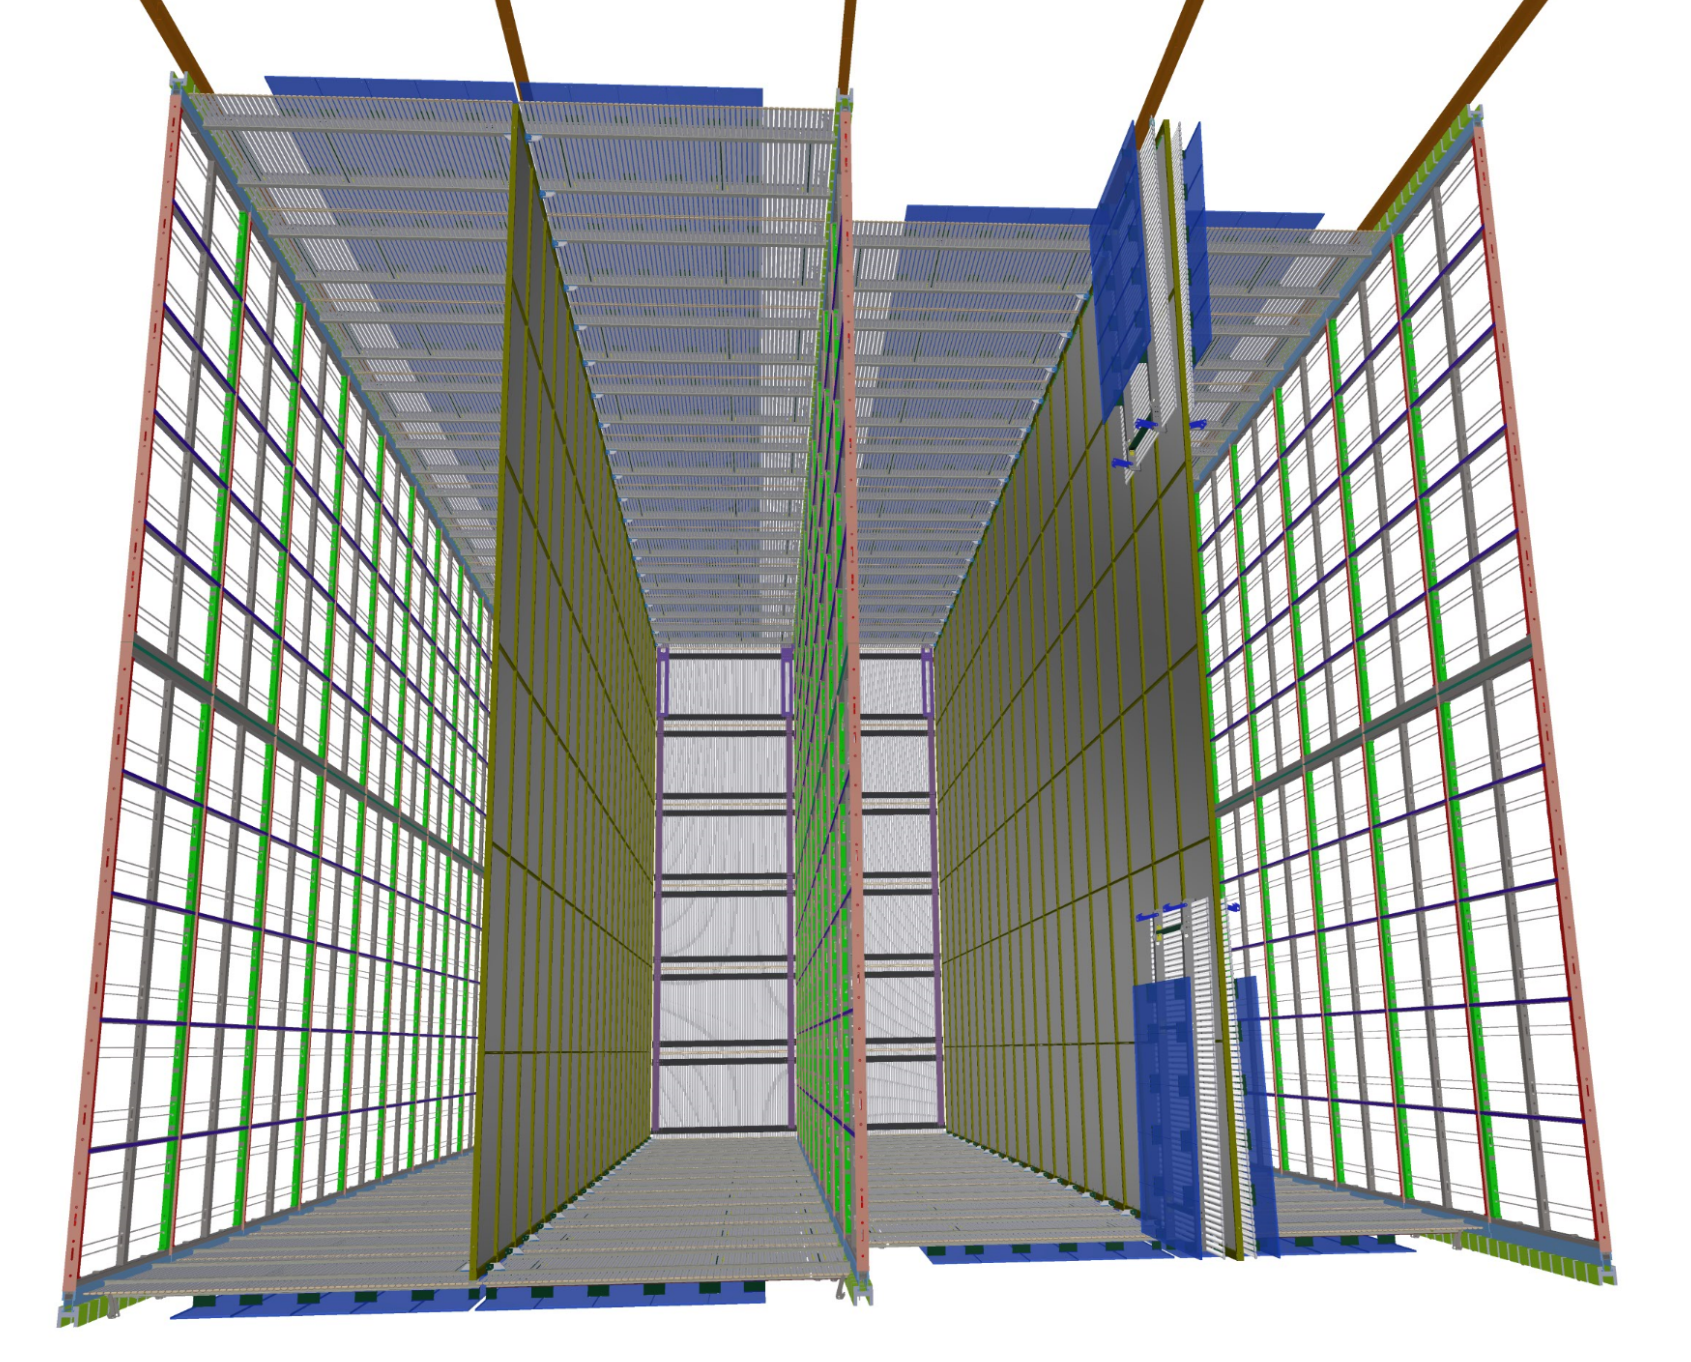
\includegraphics[width=0.8\textwidth]{dune_sp_fd}
\end{dunefigure}

The \dword{hv} consortium provides systems that operate at the full range of voltages, %all voltages, from the highest 
maximum to ground, inside the \dword{tpc} volume. As a result, its systems constitute a large fraction of the total internal structures of the \dword{tpc} itself, the principal exception being the \dwords{apa} and the \dword{pds}. In addition, the \dword{hv} system largely bounds the useful fiducial volume of the experiment, and thus plays a key role in determining the event rate for all DUNE physics processes. Mechanical and structural concerns are integrated with electrical design to meet the requirements. 

%\subsection{Design Considerations}

Two possible anode-cathode plane configurations exist for the fixed DUNE maximum electron drift length: cathode planes facing cryostat wall (C-A-C-A-C) or anode planes facing the cryostatic wall (A-C-A-C-A).  The latter configuration keeps most of the cathode plane surfaces far away from the grounded cryostat walls, reducing electrostatic breakdown risks and decreasing the total energy stored in the electric field to \SI{800}{J}.

In this configuration, energy is mostly stored in the high \efield{} region between the field cage and the nearby grounded conductors.  In an unexpected \dword{hv} breakdown, the entire \SI{400}{J} associated with one cathode could be released into a small volume of material, possibly causing physical damage.
%As an example, if this energy is converted to heat, it is sufficient to melt about 6\,mm$^3$ of stainless steel. 
It is difficult to predict the distribution of energy along a discharge path. A conservative approach treats this energy as a risk to the TPC and the cryostat membrane.  
%Given the size of the cryostat and the total TPC volume required, it is difficult to reduce this energy much further.  
Mitigating this risk entails slowing down the energy release as much as possible to minimize the potential damage by subdividing the \dword{fc} into electrically isolated modules, and constructing the cathode with highly resistive material.

Previous large \lartpc{}s (ICARUS, \microboone) have used continuous stainless steel tubes as electrodes. 
%There are disadvantages to scale this design to multi-kiloton  LArTPCs such as the DUNE Far Detector: 
Electrically, linking such electrodes to span more than \SI{100}{\m} in total length increases the stored energy each electrode has, and increases the risk of damaging the field cage components in a HV discharge. 
%Moreover, mechanically, such field cages cannot be built as completely independent modules and therefore require labor intensive steps to interconnect the electrodes, many at great heights inside the cryostat; 

Having the \dword{fc} divided into mechanically and electrically independent modules eases the construction and assembly of the \dword{fc}, and also greatly restricts the extent of drift field distortion caused by a resistor failure on the divider chain of a \dword{fc} module.

If the cathode is made of metal, a \dword{hv} discharge can cause the electrical potential of the entire cathode surface to swing from its nominal bias (e.g., \SI{-180}{kV}) to \SI{0}{V} in nanoseconds. This would induce a large current into the analog \dword{fe} amplifiers connected to the sensing wires on the \dwords{apa} (mostly to the first induction wire plane channels). Internal study (docdb 1320) has shown that this surge of current would overwhelm the internal ESD protection in the \dword{fe} ASICs.  To reduce this induced current, we chose to construct the cathode out of material with high resistivity.  Figure~\ref{fig:cpa-frame-discharge} shows the release of stored energy in time and the voltage distribution of a section of the cathode at one moment in time.  To minimize the induced current to the amplifiers, the surface resistivity should be raised until the ionization current from the TPC starts to cause significant voltage drop along the cathode.  In the DUNE FD the current is dominated by $^{39}$Ar decay, and we can tolerate surface resistivity well above \SI{1}{\giga\ohm/sq}. 


\begin{dunefigure}[Simulated \dword{cpa} discharge event]
{fig:cpa-frame-discharge}
{Bottom: Simulated \dword{cpa} Discharge event on a highly resistive cathode surface (1\,G$\Omega$/$\Box$), showing the voltage distribution on a section of the cathode (2.3\,m $\times$ 12\.m) 0.2\,ms after the discharge. Top: Time dependence of removal of stored energy.}
\centering
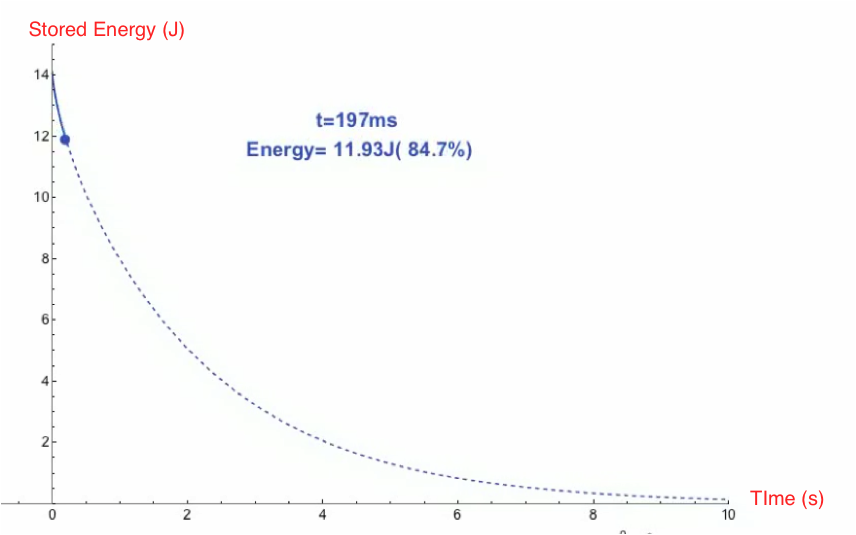
\includegraphics[width=0.6\textwidth]{A2r} \\ \vspace{30pt}    %update image with red labels
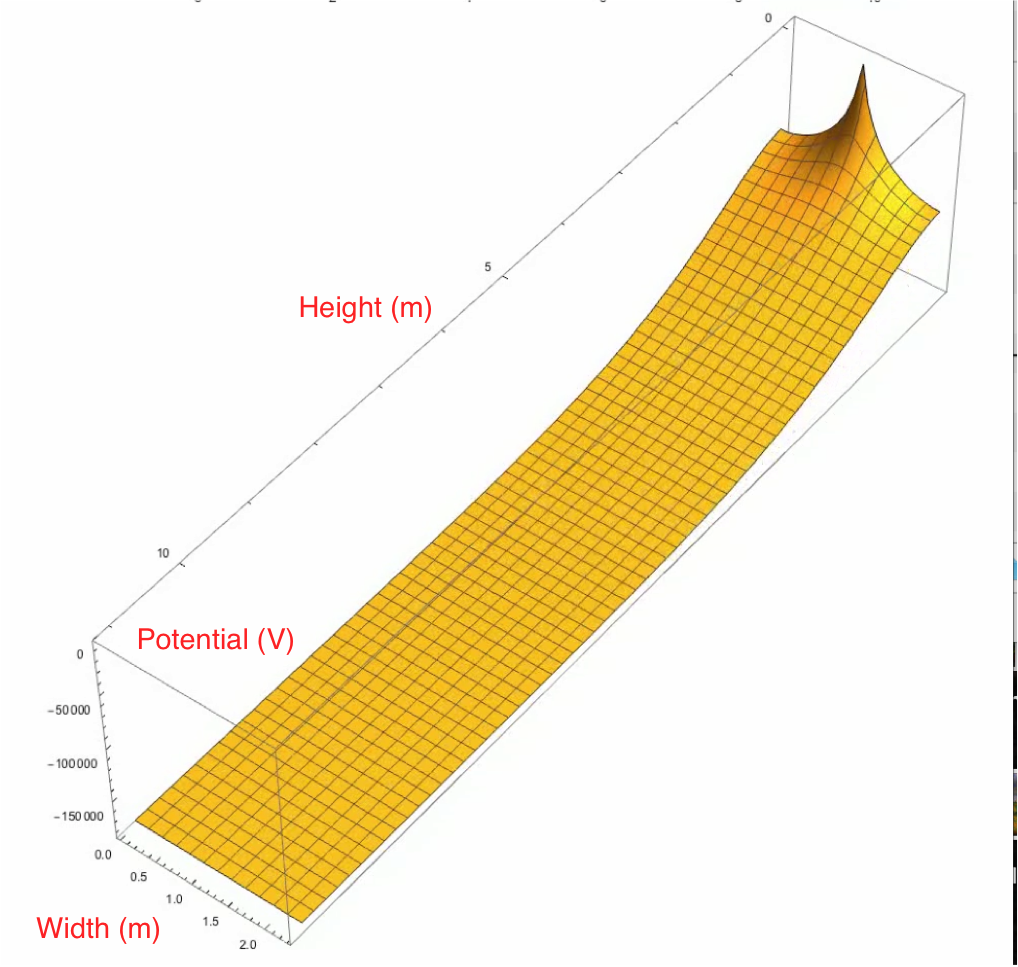
\includegraphics[width=0.5\textwidth]{A3r}
\end{dunefigure}

The SP \dword{hv} system may have modifications if problems are identified in the present design in \dword{pdsp}. Issues identified in earlier testing form the basis of an ongoing R\&D program.



%%%%%%%%%%%%%%%%%%%%%%%%%%%%%%%%%%%%%
\subsection{Design Requirements}
\label{sec:fdsp-hv-des-consid}
 
The %\dword{tpc} 
\dword{hv} system is designed to meet the physics requirements of the DUNE experiment. These are both physical requirements (such as \efield{}s that allow robust event reconstruction) and operational (a system that avoids over-complication so as to maximize the time that the detector can collect neutrino events). An important collection of the requirements affecting \dword{hv} is shown in 
Table~\ref{tab:hvphysicsreqs}.
%\fixme{the most important requirements? Could there be multiple important collections of them? Also, the way some are worded they are impossible to verify (maximize, adequate...RKP: Language here was chosen carefully.}

\begin{dunetable}
[HV system requirements]
{p{0.05\textwidth}p{0.2\textwidth}p{0.35\textwidth}p{0.15\textwidth}p{0.15\textwidth}}
{tab:hvphysicsreqs}
{\dword{hv} system requirements}   
No. & Requirement & Physics Requirement Driver & Requirement & Goal \\ \toprowrule
1 & Establish uniform minimum \efield{} in \dword{tpc} drift volume. & Limit recombination, diffusion, and space charge impacts $e$, $\mu$, $p$ particle ID.  Establish constant drift velocity and adequate \dword{s/n} on induction planes for tracking. & >\SI{250}{V/cm} & \spmaxfield \\ \colhline
 2 & Do not exceed maximum \efield{} in \dword{lar} volume. %; subsystems that have been validated under working conditions in pure \lar may exceed cited limit. 
 & Avoid damage to detector to enable data collection over long periods. & \SI{30}{kV/cm} & \dword{alara} \\  \colhline
3 & Minimize power supply ripple & Keep readout electronics free from external noise, which confuses event reconstruction.  & 0.9~mV & 0.9~mV\\ \colhline
4 &  Maximize power supply stability. & Maintain ability to reconstruct data taken over long period.  Maintain high operational uptime to maximize experimental statistics. \\ \colhline
5 & Provide adequate resistivity to create acceptable decay constant for discharge of the cathode surface and \dword{fc}.  & Avoid discharge damage to \dword{detmodule} or electronics to enable data collection over long periods. %Value is set to allow extraction of stored energy over periods of seconds. Maintain high operational uptime to maximize experimental statistics.  
& \SI{1}{\mega\ohm}/sq & \SI{1}{\giga\ohm}/sq \\ \colhline
6 & Provide redundancy in all \dword{hv} connections. & Avoid single point failures in \dword{detmodule} that interrupt data collection. & Two-fold & Four-fold \\ 
\end{dunetable}
%\fixme{This should match the list of requirements that are eventually put into the DOORS system. Anne}

%%%%%%%%%%%%%%%%%%%%%%%%%%%%%%%%
\subsection{Scope}
\label{sec:fdsp-hv-scope}

%This section discusses 
The scope of the \dword{hv} system includes the selection and procurement of materials for, and the fabrication, testing, delivery and installation of systems to generate, distribute, and regulate the voltages that
create a stable and precise \efield{} within a DUNE \dword{spmod}. % the DUNE detector volume. 

The \dword{hv} system consists of components both exterior and interior to the cryostat. The voltage generated at the \dword{hv} power supplies passes through the cables, filters, and the \dword{hv} feedthrough into the cryostat. From the voltage delivery into the cryostat, it is further distributed by components that form part of the \dword{tpc} structure. 
These components are:
\begin{itemize}
\item \dword{hv} power supply;
\item \Dword{topfc}, \dword{botfc}, and \dwords{gp};
\item \Dword{ewfc}.
\end{itemize}

\fixme{Here I propose a figure that illustrates how these cpa and fc pieces relate to each other, could be based off of figure 11. Anne}

The \dword{tpc} has two \dwords{cpa} \textit{arrays}, that span the length and height of the \dword{spmod}, as shown in Figure~\ref{fig:dune_sp_fd}. Given the modular design, each array is assembled a set of 25 adjacent \dword{cpa} \textit{planes}, which in turn are constructed of smaller pieces.  Each plane is a set of two adjacent \textit{panels} (full height, half length, as measured along the \dword{detmodule} length). Each panel consists of three stacked \textit{units}, approximately \SI{4}{\m} high by \SI{1.2}{\meter} long. The units each consist of two half-height vertically stacked resistive panels enclosed within a FR4\footnote{NEMA grade designation for flame-retardant glass-reinforced epoxy laminate material, multiple vendors, National Electrical Manufacturers Association\texttrademark{},  \url{https://www.nema.org/pages/default.aspx}.} frame.

An  installation rail supports the panels from above through a single mechanical link.

%\fixme{Consortium contributed pgraph; see Anne's below}
The sides of the drift volumes on both sides of the \dword{cpa} plane are covered by the \dword{fc} and \dword{ewfc}  modules to define a uniform drift field of \spmaxfield{}, with a increasing potential over \SI{3.5}{m} from the \dword{hv} \dword{cpa} (\SI{-180}{kV}) to ground potential at the \dword{apa} sensor planes. The cathode bias is provided by an external \dword{hv} power supply through an \dword{hv} \fdth connecting to the \dword{cpa} plane inside the cryostat.
The \dword{fc} modules come in two distinct types: the top and bottom (\dword{fc}), which run the full length of the \dword{detmodule}, and the \dwords{ewfc}, %end walls (EW's), 
which complete the detector at either end. The modules of both systems are constructed from an array of extruded aluminum open profiles supported by FRP\footnote{Fiber-reinforced plastic, a composite material made of a polymer matrix reinforced with fibers, many vendors.} (fiber-reinforced plastic) structural beams. A resistive divider chain connects adjacent metal profiles to provide a linear voltage gradient between the cathode and anode planes.  The \dword{topfc} and \dword{botfc} modules are nominally  \SI{2.3}{\meter} wide by  \SI{3.5}{\meter} long. At the ends, the \dword{ewfc} modules are \SI{3.5}{\meter} wide by \SI{1.5}{\meter} in height.

Structurally, the frames of the cathode and field cages are made from materials with similar thermal expansion coefficients, minimizing issues of differential thermal expansion. The field cage frames support aluminum profiles but these are restrained at only one location and are allowed to float within the frame.
%Cold testing of a \dword{cpa}, with monitoring of its geometry and electrical resistance is documented in DocDB 2338. In addition, Docdb 1504 documents the testing at cryogenic temperatures of kapton/FR4 laminates and the shrinkage of the detector was examined in Docdb 6011.
%Each \dword{topfc} and \dword{botfc} module is nominally \SI{2.3}{\m} wide by  \SI{3.5}{\m} long (along the \dword{detmodule} length). 
The \dwords{ewfc} modules, each \SI{1.5}{\m} high by \SI{3.5}{\m} wide (along the drift volume dimension), stack eight units high to cover the \tpcheight{} height of the \dword{tpc}.  
Extensive tests have been performed of mechanical and electrical properties of materials used in the \dword{hv} system.  These are fully documented elsewhere\fixme{Add to bib: \textit{CPA Electrical Connections Cold Test}, DUNE DocDB 2338; \textit{CPA and FC Design}, DUNE DocDB 1504; \textit{Technical Review: Mechanical Specifications for \dword{pdsp} \dword{fc} test in \dword{35t} at \fnal}, DUNE DocDB 1601.
}

The \dwords{cpa} and \dwords{apa} support the \dword{topfc} and \dword{botfc} modules, whereas
%The \dword{topfc} and \dword{botfc} modules are supported by the \dwords{cpa} and \dwords{apa}. 
%The \dwords{ewfc} modules are \SI{1.5}{\meter} tall by \SI{3.5}{\meter} long. They are stacked eight units high to cover the \SI{12}{\meter} height of the \dword{tpc}.  
installation rails above the \dwords{apa} and \dwords{cpa} support the \dword{ewfc} modules. 
%are supported by the installation rails above  the \dwords{apa} and \dwords{cpa}, which are part of the \dword{dss}. 
A \dlong{gp} consisting of tiled, perforated stainless steel sheets % panels %is mounted on 
runs along the outside surface of each of the %top and bottom \dword{fc} modules 
\dword{topfc} and \dword{botfc}, with a \SI{20}{\centi\meter} clearance. 

%For ease of understanding the rather complex physical layout of the systems comprising the \dword{hv} and \efield{} hardware, 
Tables~\ref{tab:cpaparts} and~\ref{tab:fcparts} contain summaries of terminology and parts.

\begin{dunetable}
[\dword{hv} \dword{cpa} components]
{p{0.4\textwidth}p{0.12\textwidth}
p{0.12\textwidth}p{0.32\textwidth}}
{tab:cpaparts}
{\dword{hv} Cathode Plane Components} 
Component and Quantity &  Length (z) & Height (y) & Per \dword{spmod} \\ \toprowrule
\dword{cpa} array (2 per \dword{spmod}) & \SI{58}{\meter} & \SI{12}{\meter} & 2  \\ \colhline
\dword{cpa} plane (25 per \dword{cpa} array)  & \SI{2.3}{\meter}  &\SI{12}{\meter} & 50  \\ \colhline
\dword{cpa} panel (2 per \dword{cpa} plane)  & \SI{1.2}{\meter}   & \SI{12}{\meter} & 100  \\ \colhline
\dword{cpa} unit (3 per \dword{cpa} panel)  & \SI{1.2}{\meter}  & \SI{4}{\meter} & 300 \\ \colhline
\dword{cpa} RP (2 per \dword{cpa} unit)  & \SI{1.2}{\meter}  & \SI{2}{\meter} & 600 \\
\end{dunetable}


\begin{dunetable}
[\dword{hv} \dword{fc} components]
{p{0.37\textwidth}p{0.07\textwidth}p{0.07\textwidth}p{0.07\textwidth}p{0.07\textwidth}
p{0.1\textwidth}p{0.15\textwidth}}
{tab:fcparts}{\dword{hv} Field Cage Components}
Component & Count & Length (z) & Width (x) & Height (y) & Submodules & Grand Total \\ \toprowrule
\dword{fc} (Top/Bottom Field Cage) & 200 & 2.3 m & 3.5 m & - & 57 & 200 \\ \colhline
\dword{fc}-Profiles (per \dword{fc}) & 57 & 2.3 m & - & - & - & 11400 \\ \colhline
Ground Plane Modules (per \dword{fc}) & 5 & 2.3 m & 0.7 m & - & - & 1000 \\ \colhline
EW-Plane (Endwall Field Cage) & 2 & - & 14.4 m & 12 m & 4 & 2 \\ \colhline
EW (per EW-Plane) & 4 & - & 3.5 m & 12 m & 8 & 8 \\ \colhline
EW-Modules (per EW) & 8 & - & 3. m & 1.5 m & 57 & 64 \\ \colhline
EW-Profiles (per EW-Module) & 57 & - & - & 1.5 m & - & 3648 \\
\end{dunetable}
%%%%%%%%%%%%%%%%%%%%%%%%%%%%%%%%%%%%%%%%%%%%%%%%%%%%%%%%%%%%%%%%%%%%
\section{HV System Design}
\label{sec:fdsp-hv-design}

\subsection {High Voltage Power Supply and Feedthrough}
The \dword{hv} delivery system consists of
\begin{itemize}
\item two power supplies,
\item \dword{hv} cables,
\item filter resistors, and
\item \dword{hv} feedthroughs into the cryostat.
\end{itemize}

For \dword{hv} delivery, two power supplies are used to generate the voltage, one for each \dword{cpa} array. 
This separated setup more easily accommodates different running conditions and helps isolate any instabilities. %In addition, t
The cryostat design has two feedthrough ports for each \dword{cpa} array, one at each end of the cryostat. The spare, downstream port provides redundancy against any failure of the primary \dword{hv} delivery system. 
%In the event only one power supply is available, the system will be run by using a \dword{hv} splitter outside of the cryostat while another power supply is procured. 

Each \dword{cpa} connects to two drift volumes in parallel, presenting a net resistance of \SI{1.14}{\giga\ohm} to each supply. At the nominal \SI{180}{kV} cathode voltage, each power supply must provide \SI{0.16}{mA}.

The planned power supply model for the \dword{spmod} is similar to the power supply\footnote{Heinzinger, PNC HP200000 \dword{hv} power supply, Heinzinger\texttrademark{} Power Supplies, \url{http://www.heinzinger.com/}.} used on \dword{pdsp}, with a maximum output voltage of \SI{200}{kV} and a maximum current draw of \SI{0.5}{mA}.  An %additional 
option is an existing \SI{300}{kV}, \SI{0.5}{mA} model from the same vendor.
The \dword{hv} cables are commercially available models compatible with the selected power supplies. 

%The \dword{hv} cables will be either Dielectric Sciences model number 2134 capable of \SI{200}{kV} DC or 2236 capable of \SI{320}{kV} DC. 
%ielectrThe \dword{hv} cables are preferred to be Dielectric Sciences model number 2134 capable of \SI{200}{kV} DC.  A back up plan is to use model 2236 capable of \SI{320}{kV} DC. 

Filter resistors are placed in between the power supply and the feedthrough.  Along with the cables, these resistors reduce the discharge impact by partitioning the stored energy in the system.  The resistor-cable assembly also serves as a low-pass filter reducing the \SI{30}{kHz} voltage ripple on the output of the power supply.  With filtering, such supplies have been used successfully in other \lartpc experiments, such as \microboone and ICARUS.

Figure~\ref{fig:ps_filter_ft_schematic} provides a sample schematic of the \dword{hv} supply circuit.

\begin{dunefigure}[A schematic showing the \dword{hv} delivery system to the cryostat.]  %The two filters are placed such that one is near the power supply and one is near the feedthrough.
{fig:ps_filter_ft_schematic}
{Right:  A schematic showing the \dword{hv} delivery system to the cryostat (Credit:  SEL). %The two filters are places such that one is near the power supply and one is near the feedthrough. 
One of the two filters sits near the power supply; the other sits near the feedthrough. Left:   %An example 
A Heinzinger power supply (Credit: H.~Wang).}
%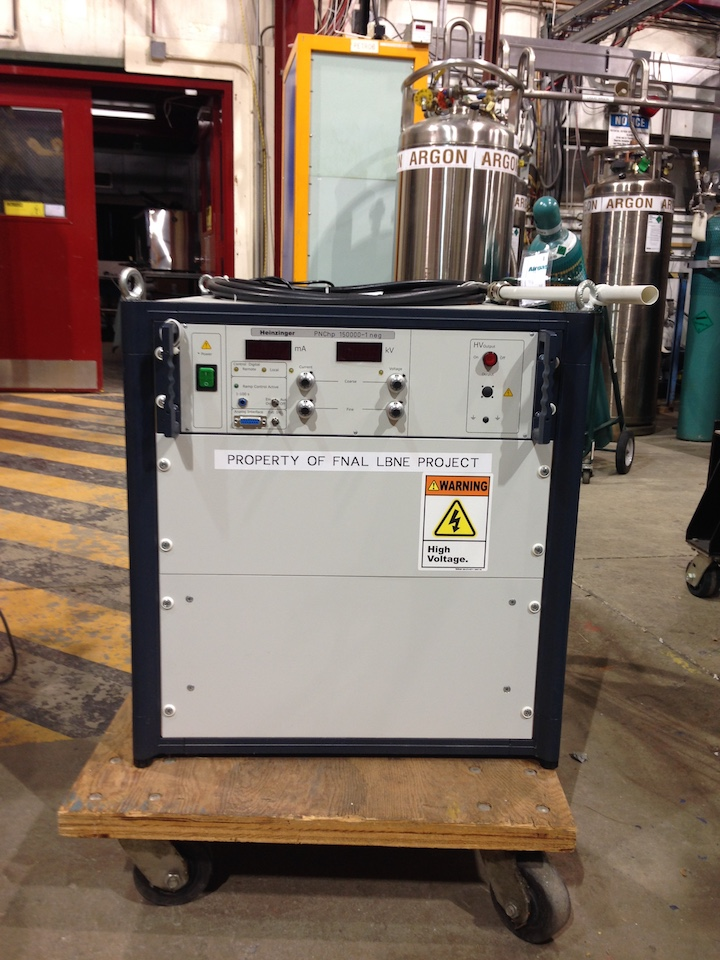
\includegraphics[width=0.2\textwidth]{heinzy}
%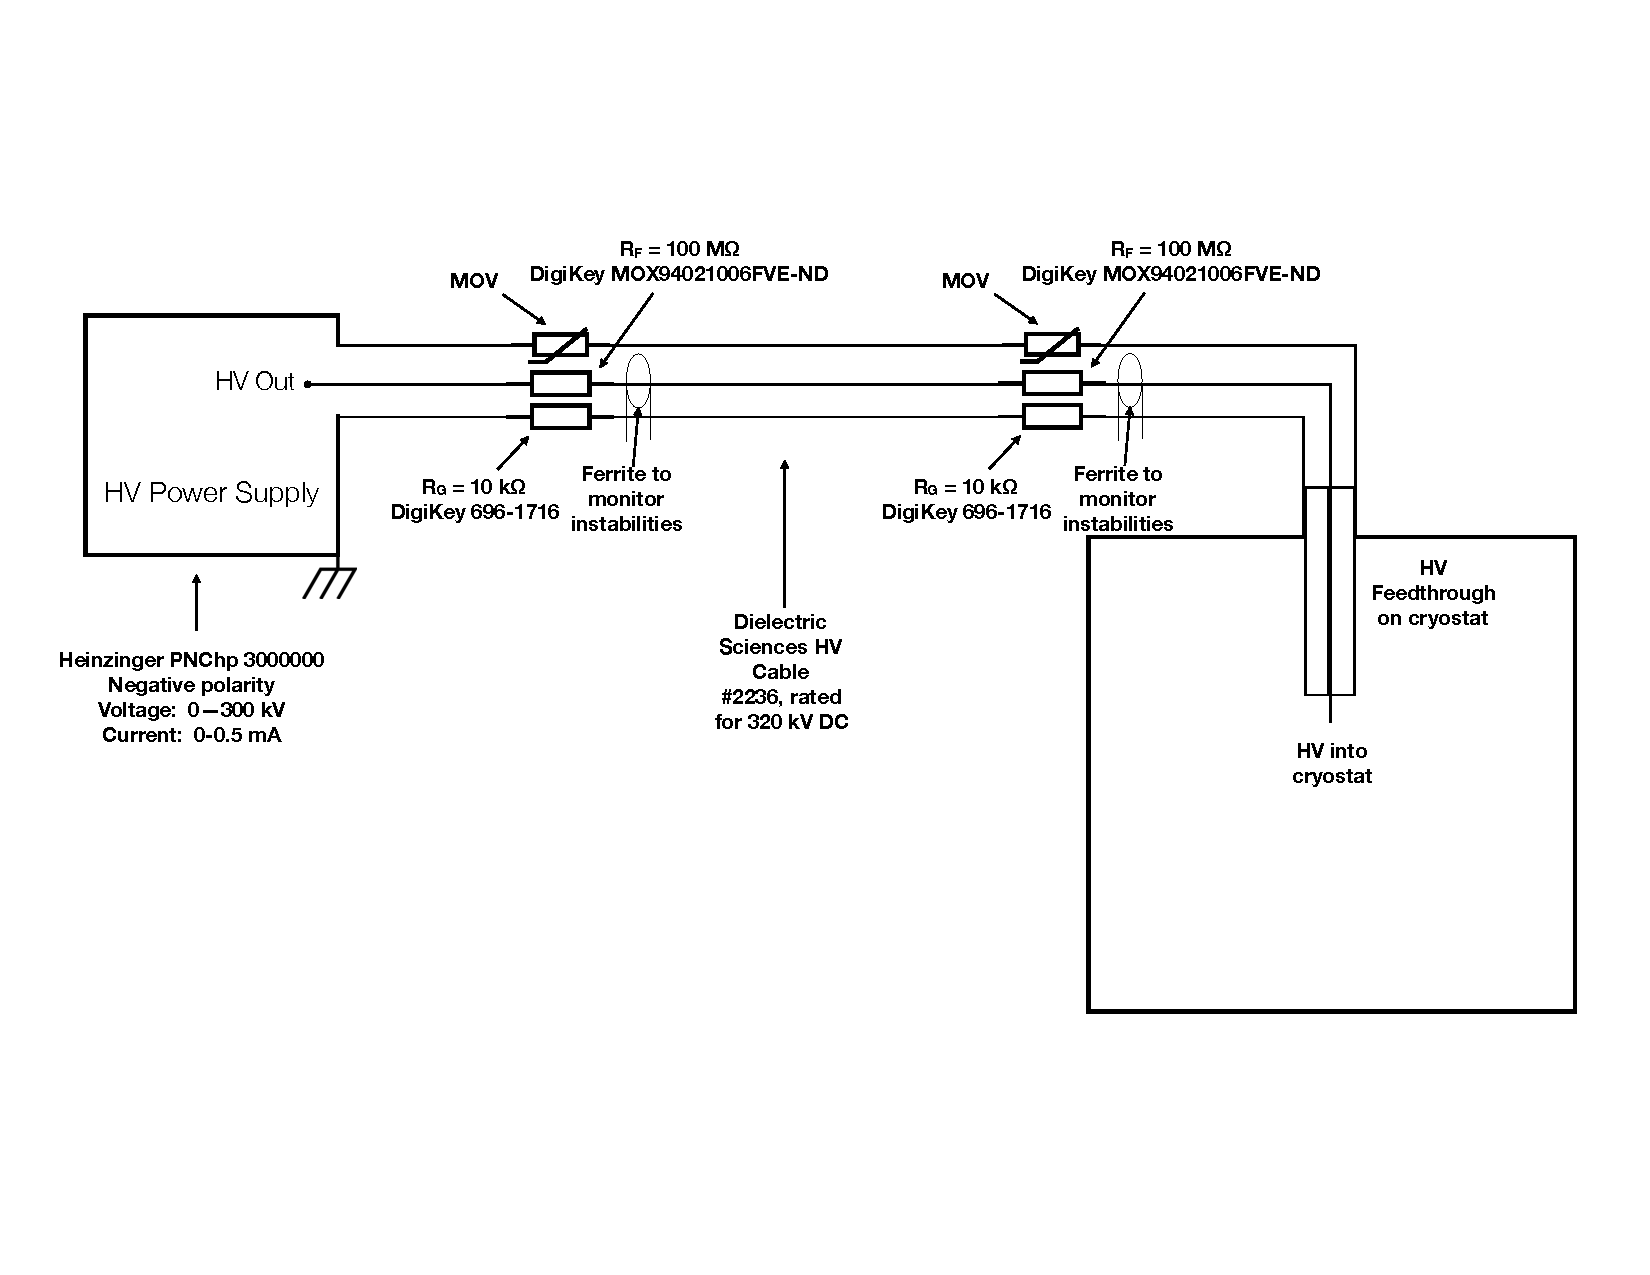
\includegraphics[width=0.7\textwidth]{ps_filter_ft_schematic}  %requested image edits by DeMuth
\begin{minipage}{5in}
  \centering
  $\vcenter{\hbox{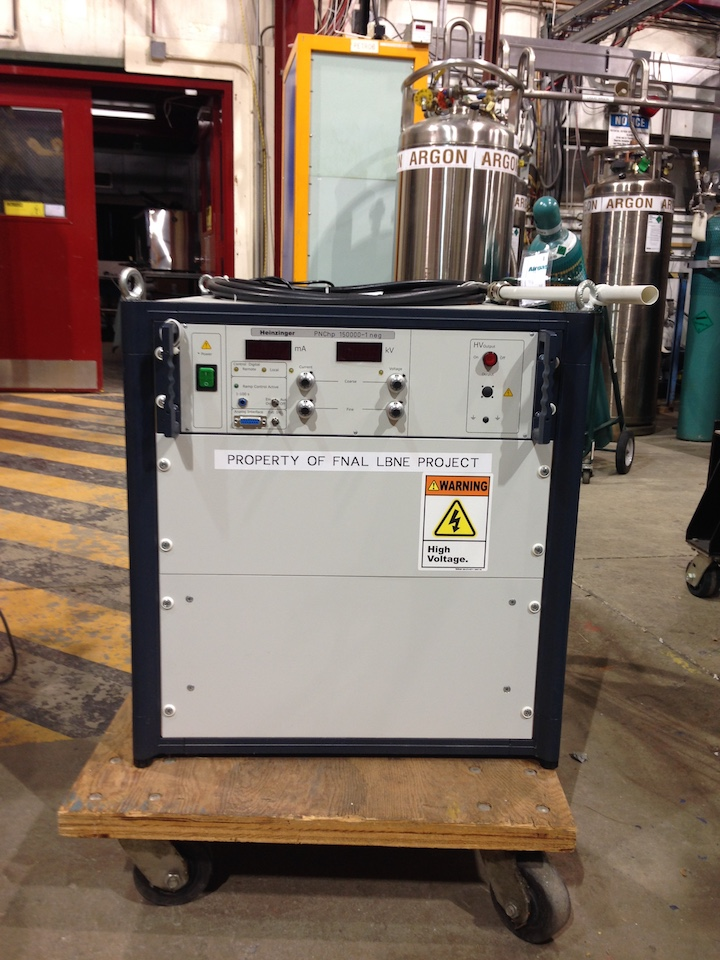
\includegraphics[width=0.2\textwidth]{heinzy}}}$
  \hspace*{.2in}
  $\vcenter{\hbox{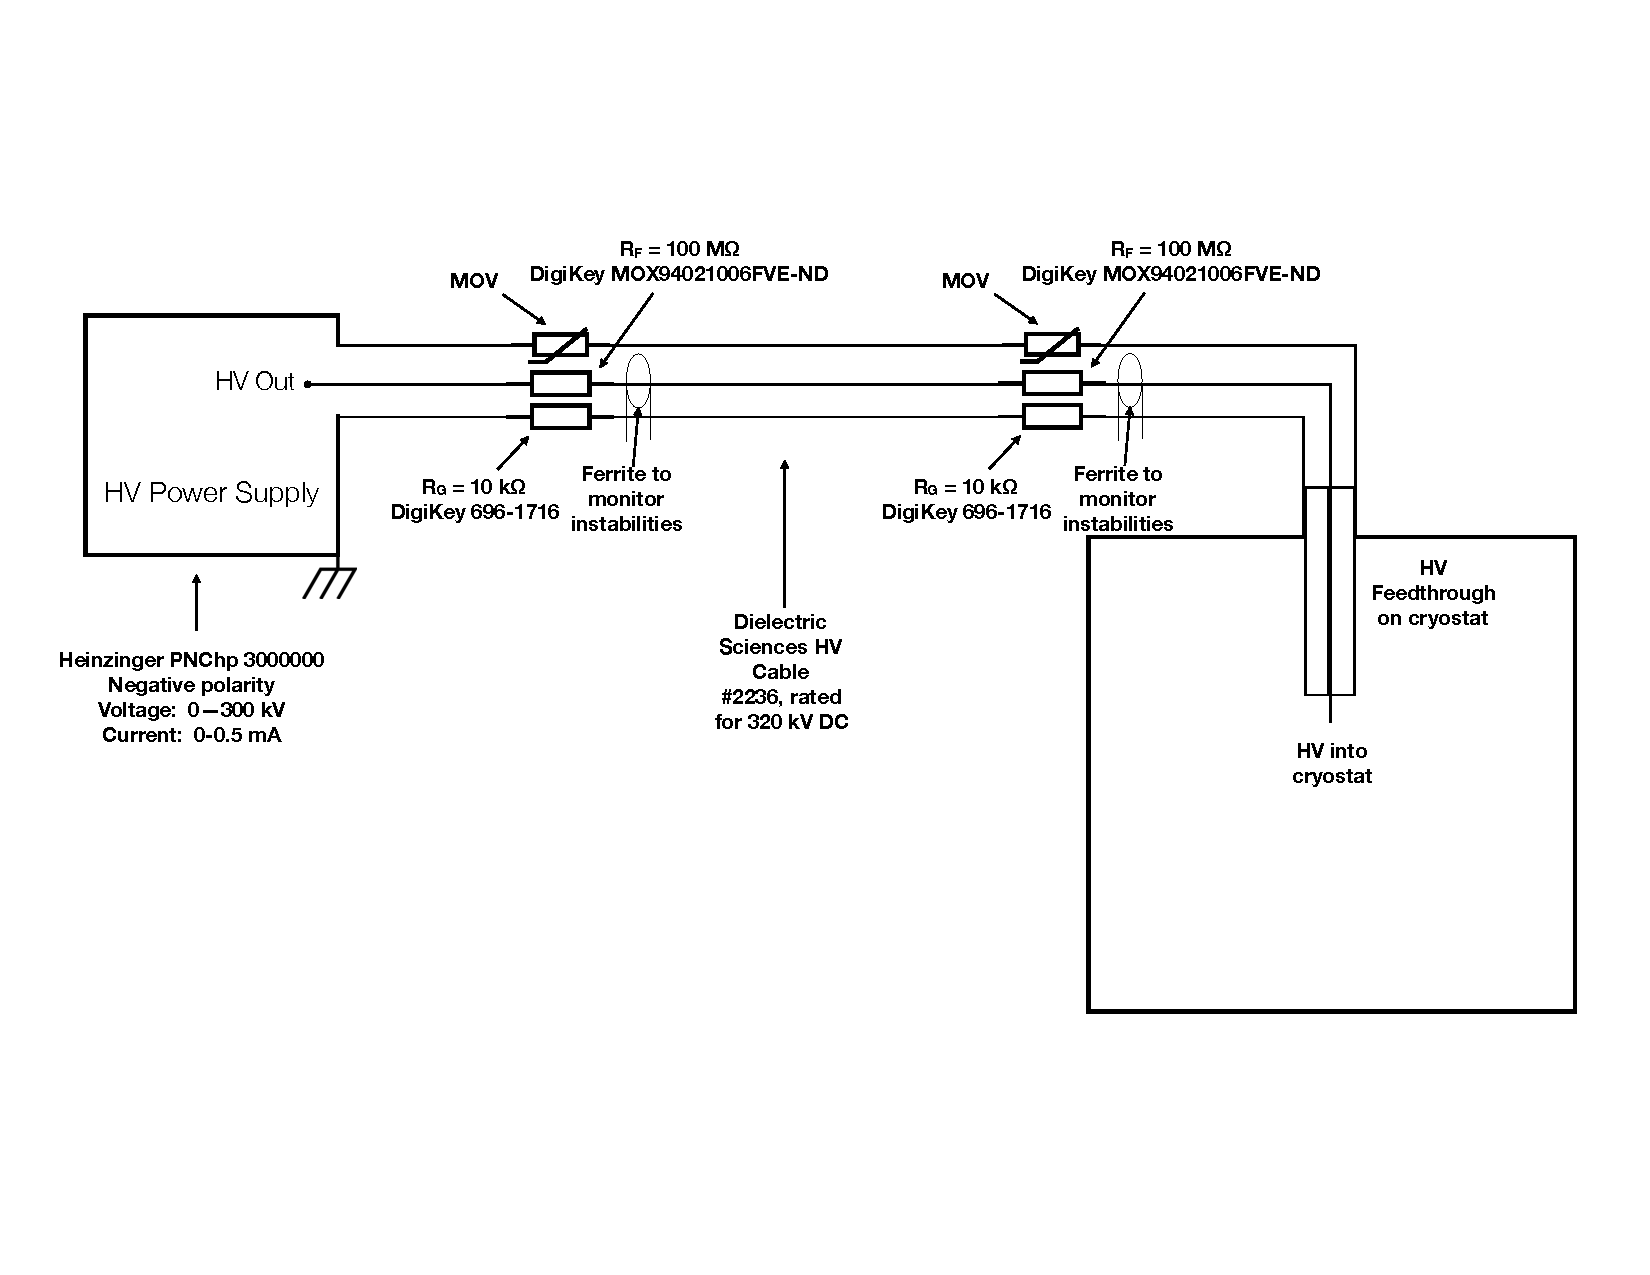
\includegraphics[width=0.7\textwidth]{ps_filter_ft_schematic}}}$
\end{minipage}
\end{dunefigure}
The requirement %of 
on low electronics noise sets the upper limit of residual voltage ripple on the cathode to be \SI{0.9}{mV}.  Typically, commercial supplies %can 
specify  that the ripple variation is limited to % less than or equal to $0.001\%V_{nom} \pm 50$ mV.  
\SI{.0001}{\%} around an absolute precision in nominal voltage of plus or minus \SI{50}{mV}.
%
Assuming cable lengths of \SI{30}{m} and \SI{3}{m} between the filters themselves, and between the filter and \fdth, respectively, resistances as low as a few \si{\mega\ohm} yield the required noise reduction according to calculations and experience. % the noise reduction can be attained with resistances as low as a few M$\Omega$. 

The current plan for the filters is a cylindrical design.  %Here, an \dword{hv} resistor will be electrically connected on each end to a cable receptacle.  
Here each end of an \dword{hv} resistor is electrically connected to a cable receptacle. 
The resistor %should shall be selected to 
must withstand a large over-power condition.  Radially out from the resistor is an insulator,  %In other designs, this has been 
for which other designs have used transformer oil or ultra-high molecular weight polyethelene (UHMWPE).  The outer case of the filter is a grounded stainless-steel shell. The current filter design is shown in Figure~\ref{fig:filterAndFeedthrough}.

The \dword{hv} feedthrough %will be 
is based on the successful ICARUS design, \fixme{ref} which has been adapted for \dword{pdsp}.  The voltage is transmitted by a stainless steel center conductor.  On the warm side of the cryostat, this conductor mates with a cable end.  Inside the cryostat, the end of the center conductor has a spring-loaded tip that %will 
contacts a receptacle cup mounted on the cathode, delivering \dword{hv} to the field cage.  The center conductor of the \fdth is surrounded by UHMWPE. A drawing is shown in Figure~\ref{fig:filterAndFeedthrough}.

\begin{dunefigure}[Drawings of the \dword{hv} filters and feedthroughs]{fig:filterAndFeedthrough}
{Left:  Drawing of a \dword{hv} filter (Credit:  A.~Renshaw). Right:  \dword{hv} feedthrough drawing (Credit:  (F.~Sergiampietri).}
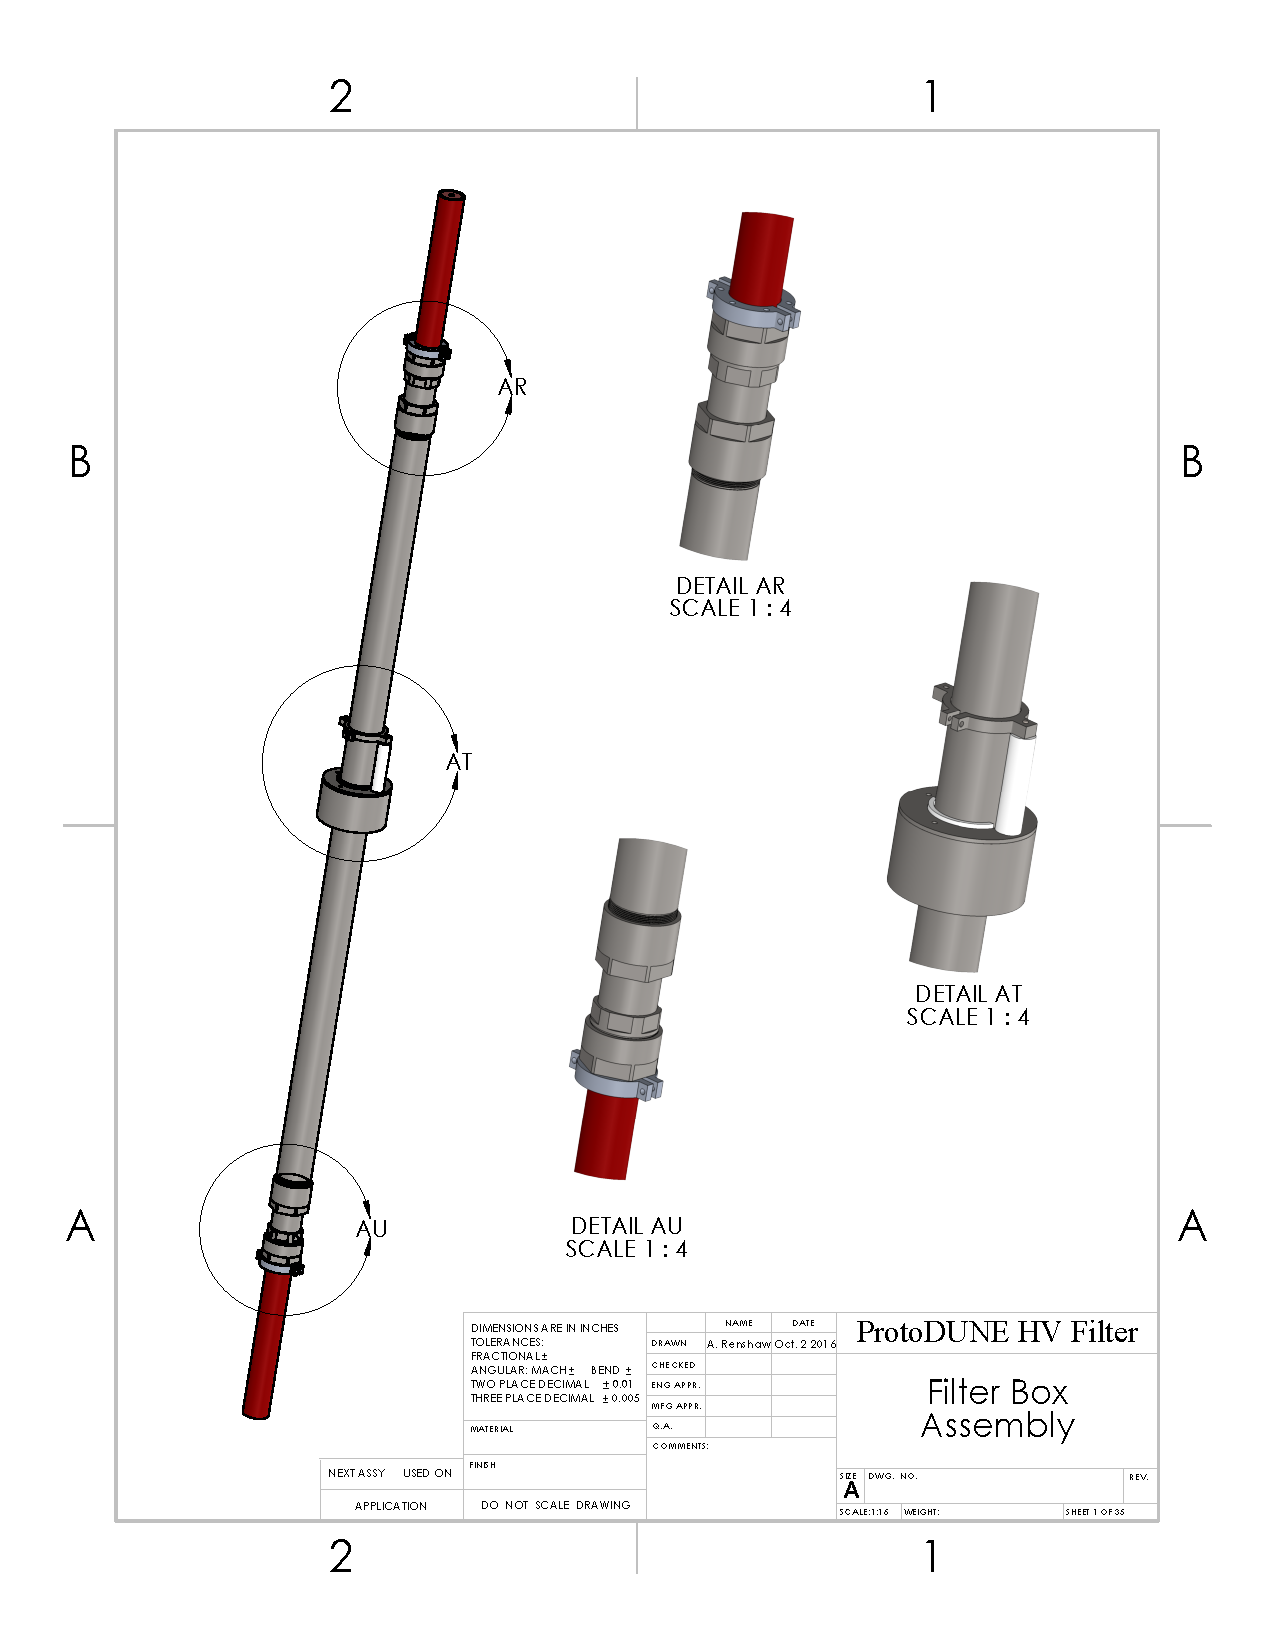
\includegraphics[width=0.3\textwidth]{pdFilters}
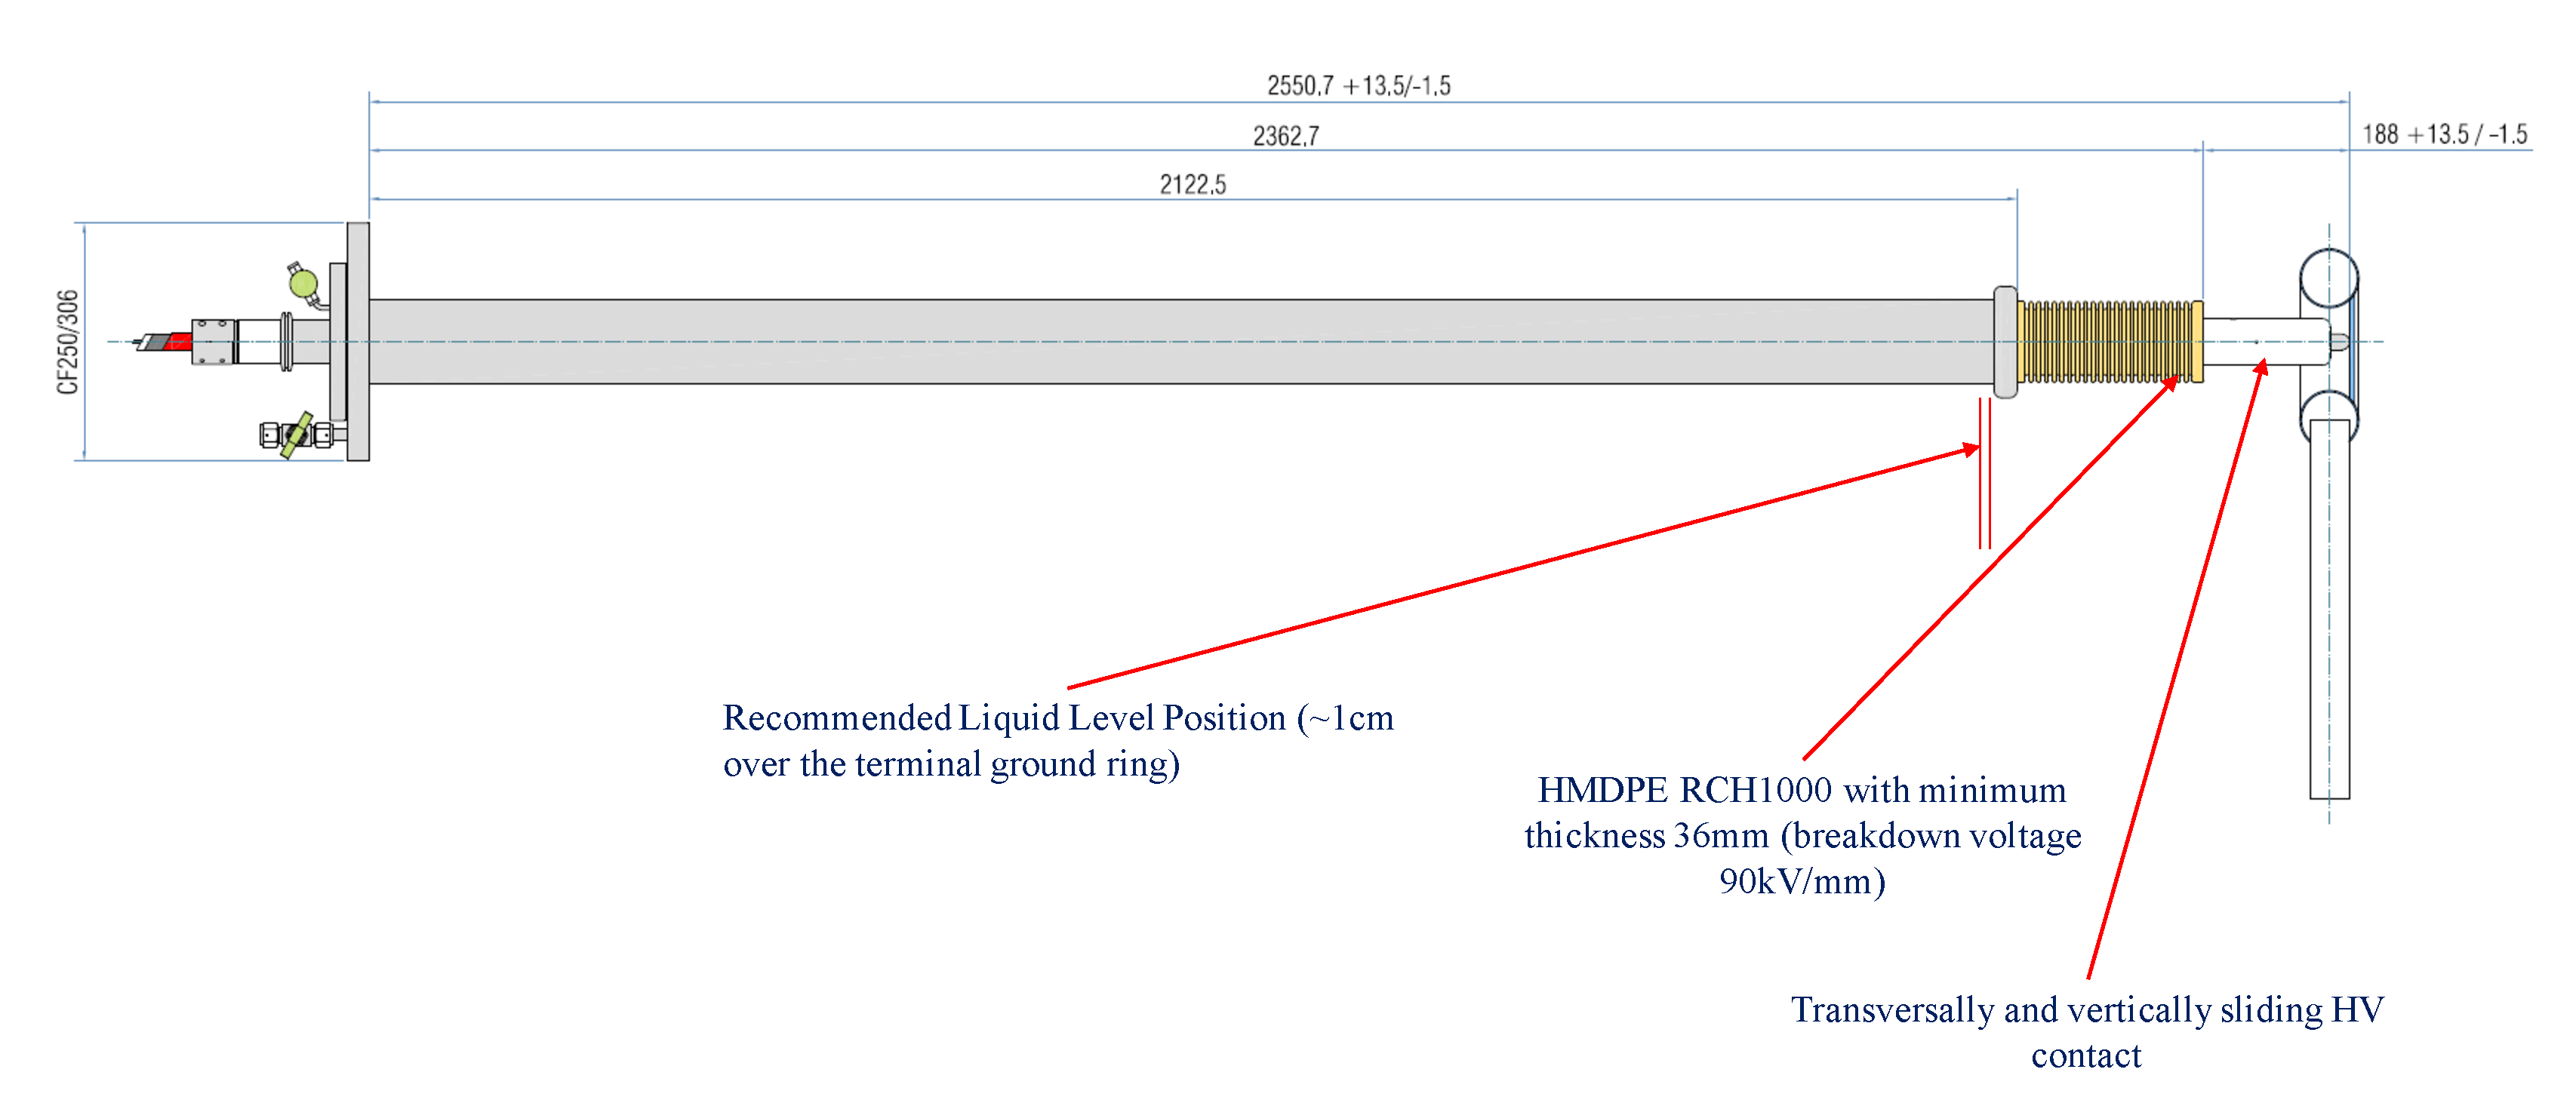
\includegraphics[width=0.6\textwidth]{francosHVFT}
\end{dunefigure}

The upper bound of operating voltage on a feedthrough is, to first order, set by the maximum \efield{} on the feedthrough.  This \efield{} is reduced by increasing the insulator radius.  For the target voltage, the feedthrough uses a UHMWPE cylinder of approximately \SI{15}{cm} diameter.  In the gas space and into at least \SI{15}{\centi\meter} of the liquid, the insulator is surrounded by a tight-fitting stainless steel ground tube.  The ground tube has a \SI{25}{\centi\meter}  Conflat (an industry standard) flange  welded on for attachment to the cryostat.

%Orig pgraph
%There will be multiple devices used to monitor the \dword{hv}.  Outside of the cryostat, the power supply and cable-mounted toroids will be used.  The Power Supply units typically have sensitivities down to 10's of nA in current read-back capability.  The units are able to sample the current and voltage every \SI{300}{ms}.  The cable-mounted toroids are sensitive to fast changes in current and can be monitored when desired.  The polarity of the signal also points to whether the current-drawing feature is upstream or downstream of the toroid.

Outside of the cryostat, the \dword{hv} power supply and cable-mounted toroids will monitor the \dword{hv}.    The power supplies %units 
typically have sensitivities down to tens of \si{\nano\ampere} in current read-back capability 
\fixme{`in read-back `mode'? or `with' read-back capability? RKP: Believe language clear as written.} and are able to sample the current and voltage every \SI{300}{\ms}.  The cable-mounted toroids are sensitive to fast changes in current; %and can be monitored. when desired.  
the polarity of a toroid's signal %also points to whether 
indicates the location of the current-drawing feature as either upstream or downstream of it.  Experience from the \dword{35t} installation suggested sensitivities to changing currents with a timescale between \SIrange{0.1}{10}{\micro\s}, providing information on the timescale of any current changes.

Inside the cryostat, pick-off points near the anode will monitor the current %going down 
in each resistor chain.  Additionally, the voltage of the \dwords{gp} above and below each drift region can be equipped to diagnose problems via a high-value resistor connecting the \dword{gp} to the cryostat.  In the \dword{35t}, such instrumentation provided useful information on \dword{hv} stability and where any stray charge was flowing.

%The external commercial \dword{hv} components will be rated at a sufficient voltage to meet the drift voltage requirement (number 1 as listed in Table~\ref{tab:hvphysicsreqs}).  Additionally, the custom filters and feedthrough will be tested to ensure that they satisfy requirement (1).  Further details 
Both commercial and custom \dword{hv} components must be rated for sufficient voltage and satisfy tests to meet the requirements summarized in Table~\ref{tab:hvphysicsreqs}.  Further details on these tests are in Section~\ref{sec:fdsp-hv-qc}.

The resistances in the filters, in combination with the capacitances between the \dword{hv} system and the cathode,
 determine the attenuation of the tens of \si{\kilo\hertz} ripple from the power supply.  The filters %will be 
are designed such that the ripple is reduced to an acceptable level when installed in the complete system, thus satisfying requirement (3) that the power supply ripple is minimized.
\fixme{`minimize ripple'' is not a validatable requirement. What is the acceptable level? Or what dictates it? Anne. RKP: Addressed in collaboration comments.}

%%%%%%%%%%%%%%%%%%%%%%%%%%%%%%%%%%%%%
\subsection{Cathode Plane Assembly (CPA)}

The \dword{cpa} provides a constant potential surface at \SI{-180}{\kV} for the \dword{spmod}.  It receives its \dword{hv} from the feedthrough that makes contact with the \dword{hv} bus mounted on the \dword{cpa} frame through an attached donut assembly attached to the frame, as shown in Figure~\ref{fig:donut_cpa}. % shows the connection of the \dword{hv} input donut to the \dword{hv} bus on the \dword{cpa} frame. 
The \dword{cpa} also provides \dword{hv} to the first profile on the top and bottom \dword{fc} elements and to the \dwords{ewfc} as well. %More d
Details on the electrical connections are found in Section ~\ref{sec:fdsp-hv-design-interconnect}.

\begin{dunefigure}[\dword{hv} input donut connection to \dword{cpa}]{fig:donut_cpa}{\dword{hv} input donut connection to \dword{cpa}.}
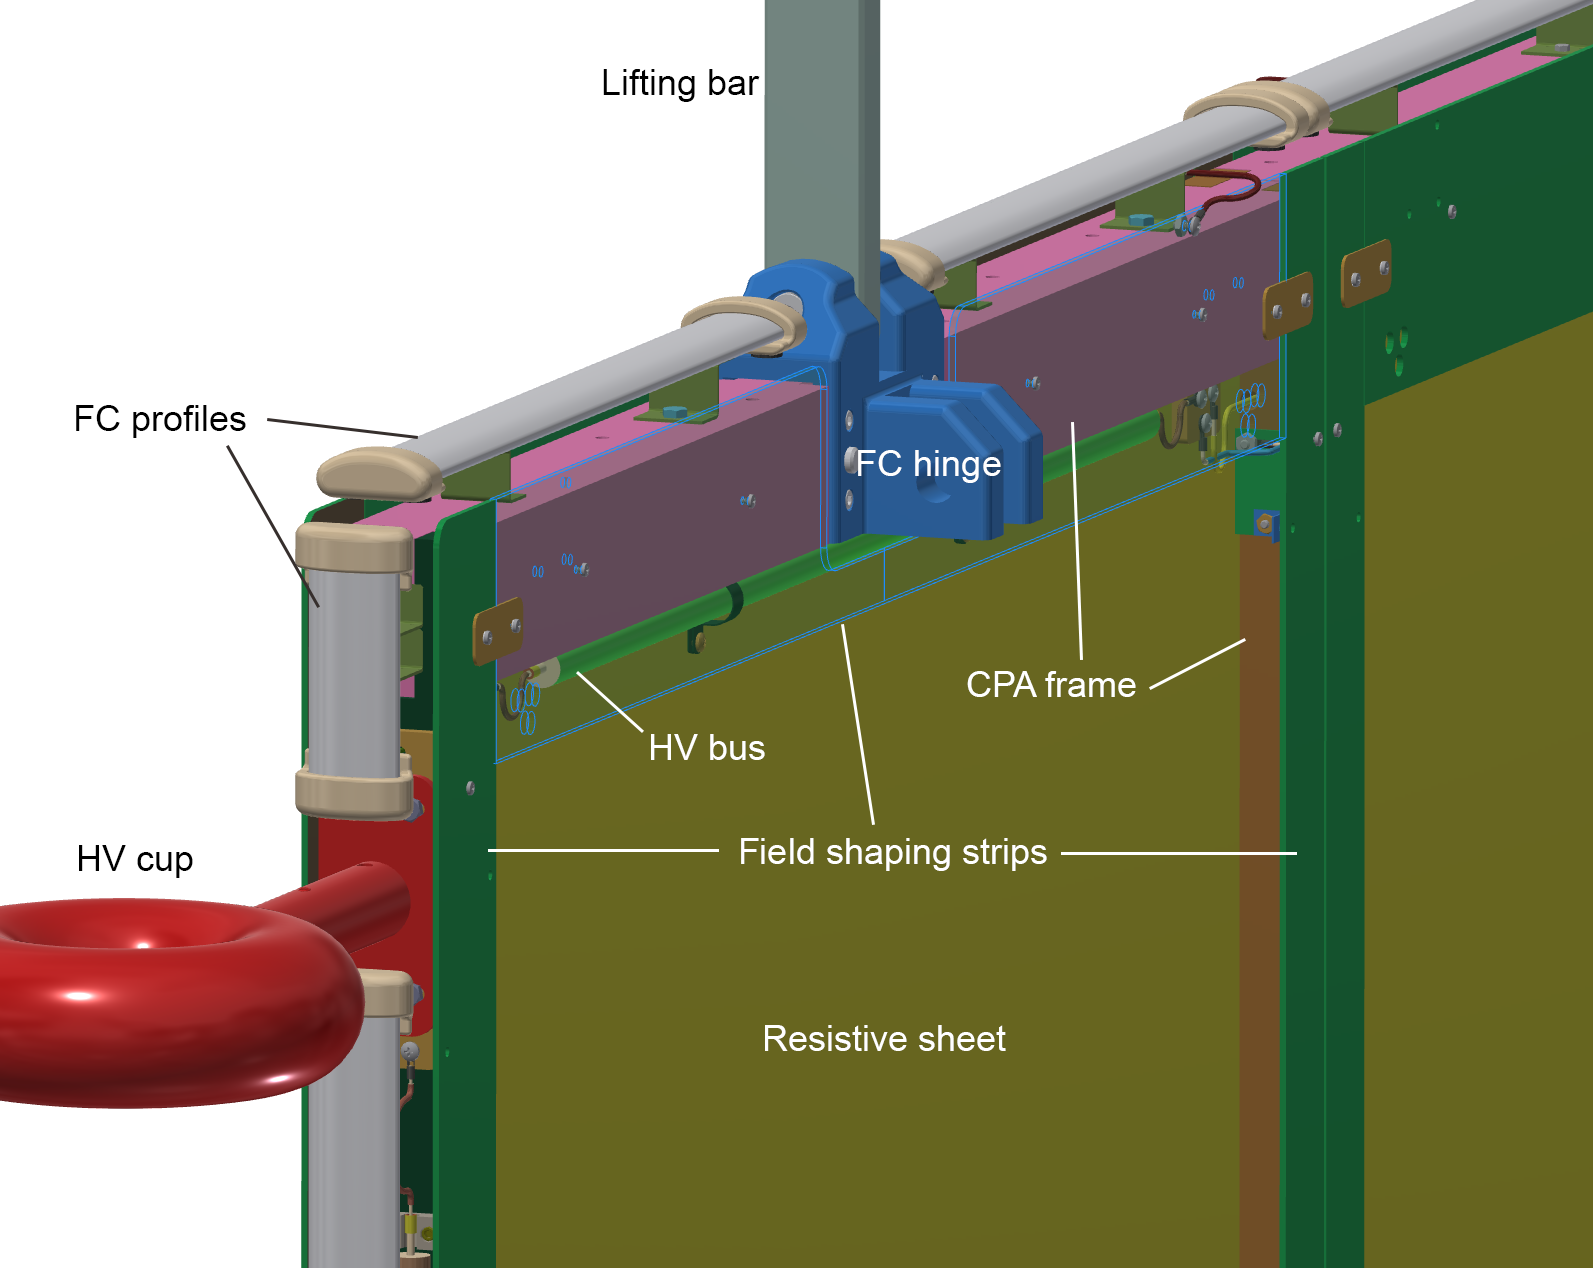
\includegraphics[width=0.6\textwidth]{donut_cpa2} %{ was Latest3D}
\end{dunefigure}

Ideally, the cathode would be constructed from a large thin resistive sheet.  However, inside the cryostat, there is a moderate convective flow of the \lar that can produce a small pressure difference across the cathode surface.  To maintain the position and flatness of the cathode, the cathode surface must be reinforced for stiffness.  This is accomplished using \SI{6}{cm} thick FR-4 frames at \SI{1.2}{m} intervals. Since FR4 is a good insulator at cryogenic temperature with a different dielectric constant that \lar, the presence of the frame causes a local \efield distortion that can become pronounced if the frame surface charges up as a reult from ionization in the TPC.  To minimize this distortion, a resistive field shaping strip is placed on the cathode frame and biased at a different potential.  Figure~\ref{fig:fss_concept} illustrates the drift field uniformity improvement with the field shaping strips.

\begin{dunefigure}[\dword{fss} concept]{fig:fss_concept}{A comparison of three cathode cross sections to illustrate the benefit of the \dword{fss}. Both equipotential lines (horizontal) and \efield{} lines (vertical) are shown.  The amplitude of the \efield{} is shown as color contours. Each color contour is a 10\% step of the nominal drift field.  The gray rectangles represent the frame and the resistive sheet in each case. Left: a conductive/resistive frame similar to that of ICARUS or SBND; Middle: an insulating frame with the insulating surfaces charged to an equilibrium state; Right: an insulating frame covered with a field shaping strip (purple) and biased at the optimum potential. }
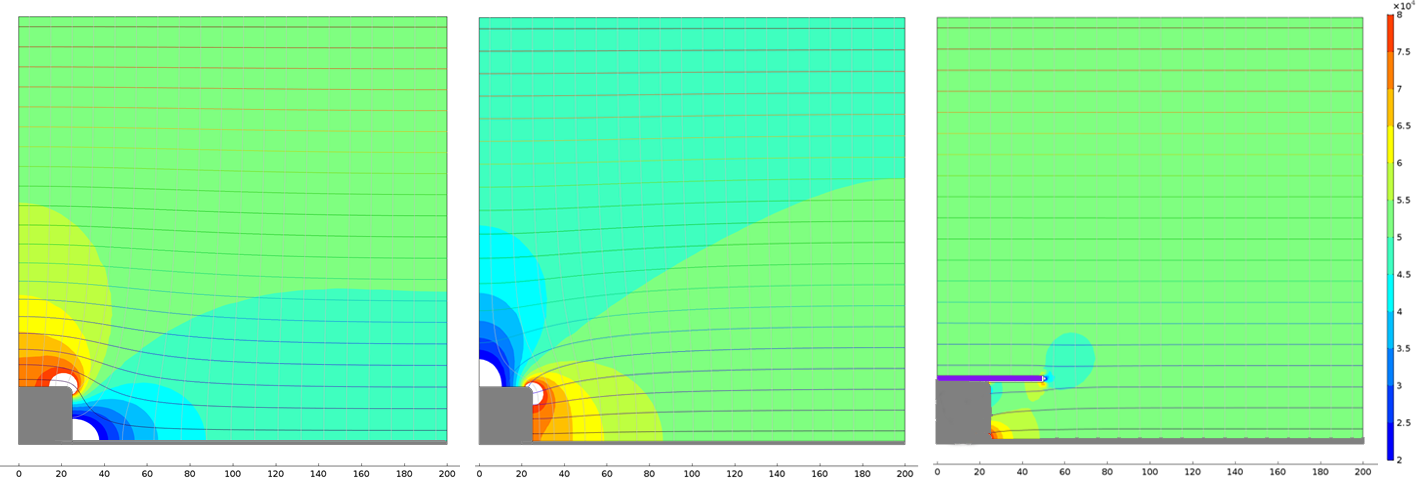
\includegraphics[width=0.9\textwidth]{field-shaping-strip-concept} %{ was Latest3D}
\end{dunefigure}

The \dwords{cpa}' constant potential surfaces are resistive panels (\dword{cpa} RPs) composed of a thin layer of carbon-impregnated Kapton\footnote{DuPont\texttrademark{}, Kapton\textsuperscript{\textregistered} polymide film,  E. I. du Pont de Nemours and Company,  \url{http://www.dupont.com/}.} 
 laminated to both sides of a \SI{3}{\milli\meter} thick FR4 sheet of \SI{1.2}{\meter}  $\times$ \SI{2}{\meter} size.  The surface resistivity of the \dword{cpa} RPs is required to be greater than 1 M\si{\ohm}/square in order to provide for slow reduction of accumulated charge in the event of a discharge.  A goal of 1 G\si{\ohm}/square for DUNE \dword{cpa} RPs extends the protection from discharges in the condition of anticipated higher stored energy at DUNE, compared to prototypes. Other \dword{hv} components of the \dword{cpa} include \dword{fss} mounted to the \dword{cpa} frames, edge aluminum profiles to act as the first elements of the field cage, and cable segments forming the \dword{hv} bus. Careful inspection of these items during the assembly process ensures that no sharp points or edges are present. The surface resistivity of the \dword{cpa} RPs and the \dword{fss} are checked multiple times during assembly -- first when the resistive panels and strips are received and after assembly into \dword{cpa} units on the table.  Coated parts that do not meet the minimum surface resistivity requirement are replaced.  This ensures that requirement (5) on Table~\ref{tab:hvphysicsreqs} is satisfied.  Figure~\ref{fig:cpa_panel-complete} shows a completed \dword{pdsp} \dword{cpa} panel on the production table ready for lifting into vertical position for mounting on its trolley.

\begin{dunefigure}[Completed \dword{pdsp} \dword{cpa} panel on production table]{fig:cpa_panel-complete}{Completed \dword{pdsp} \dword{cpa} panel on production table.}
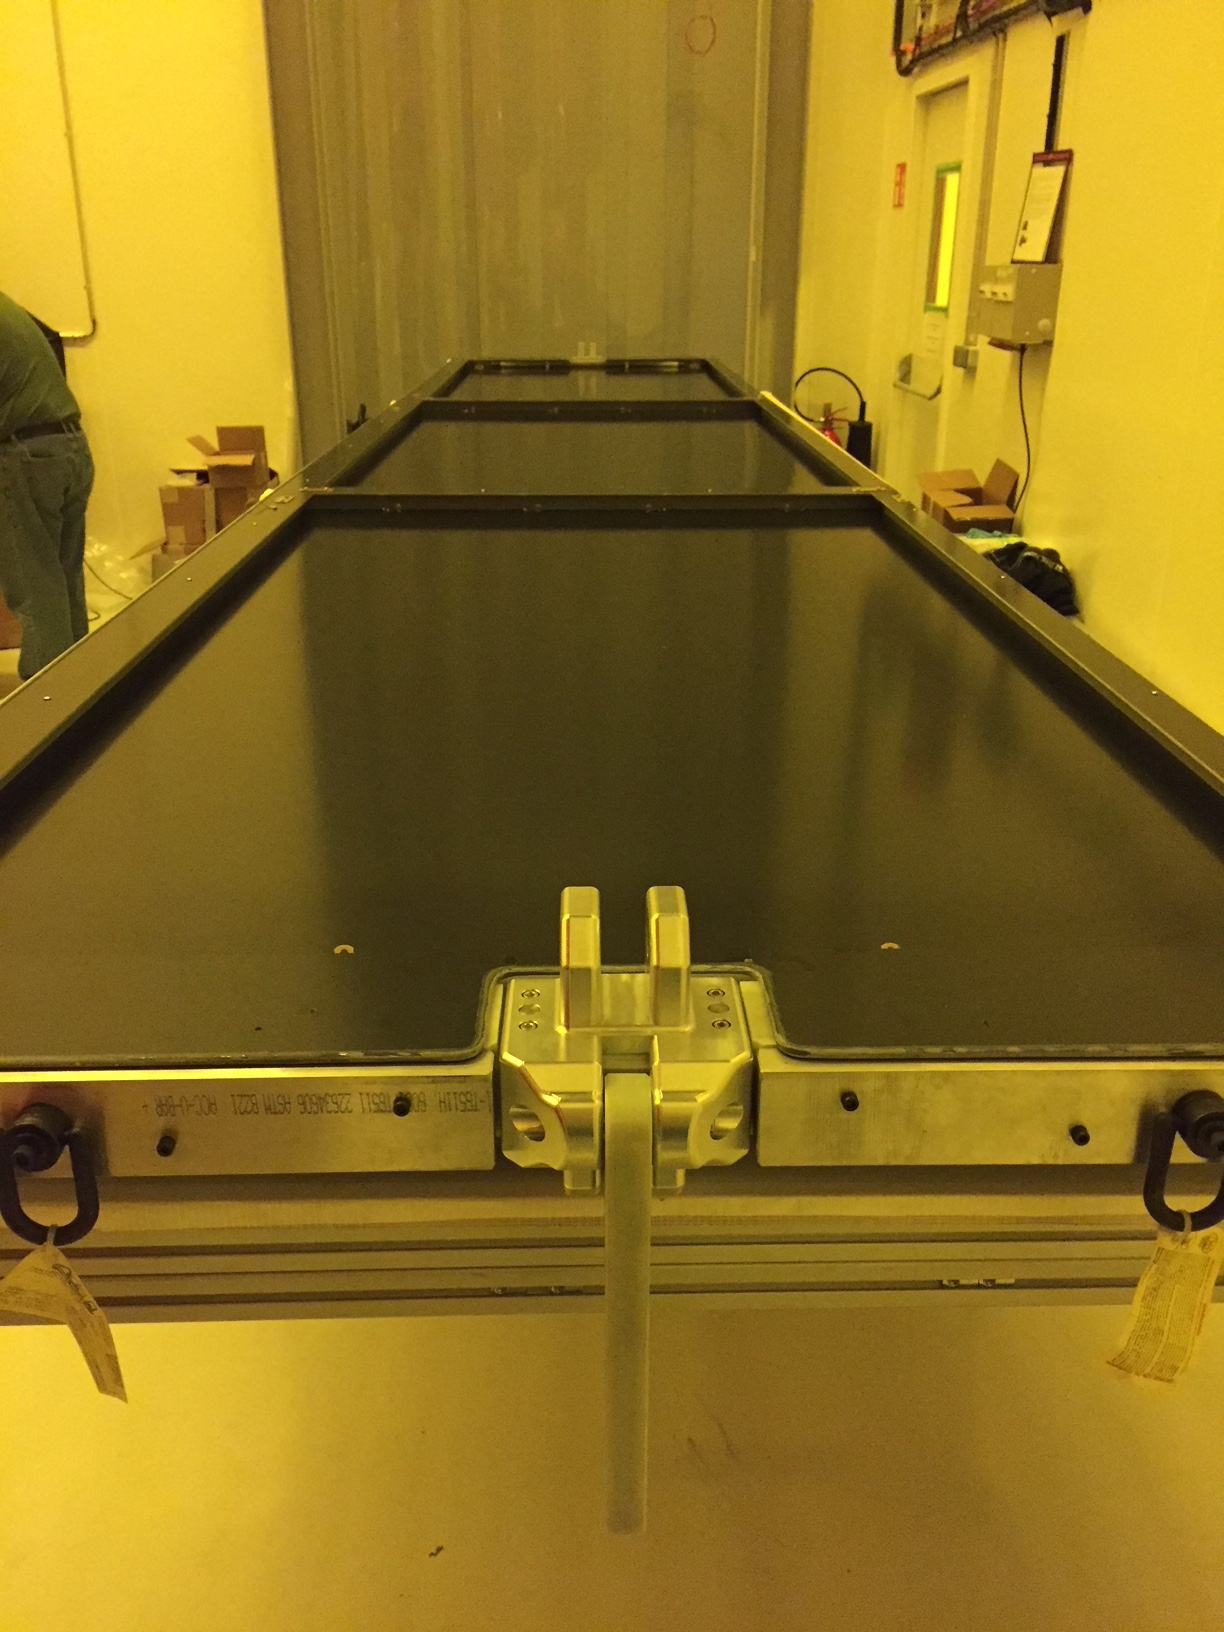
\includegraphics[width=0.5\textwidth]{cpa_panel-complete}
\end{dunefigure}

All electrical connections on the \dword{cpa} and between the \dword{cpa} and other \dword{hv} system components (top, bottom, and \dwords{ewfc}) are redundant by at least a factor of two.  Connections between RPs in a \dword{cpa} unit are four-fold redundant.  The \dword{hv} connection from the \dword{hv} power supply is a closed loop around the \dword{cpa} which can sustain at least one broken connection without loss of the cathode plane \dword{hv}.  This ensures compliance with %that 
requirement (6) of Table~\ref{tab:hvphysicsreqs}.
%is satisfied.

The \dword{cpa} frames are required to support, in addition to the \dword{hv} components, the \dword{topfc} and \dword{botfc} units attached to both sides of the \dword{cpa} panel. The arrangement and deployment of these components will be the same as in \dword{pdsp}.  
%%%%%%%%%%%%%%%%%%%%%%%%%%%%​%%%%%%%%%%%%%%%​
\subsection{Field Cages}
%%%%%%%%%%%%%%%%%%%%%%%%%
\subsubsection{General Considerations}

A uniform \efield{} is required to drift ionization electrons towards the \dwords{apa}. The \dwords{fc} consisting of field shaping electrodes form a band surrounding the top, bottom, and ends of the active drift volume. The electrodes are biased at different potentials to establish a uniform field inside the \dword{lar} volume.
The \dword{spmod} will use extruded aluminum profiles as a cost-effective way to establish the equipotential surfaces. 

For safe and stable operation of the \lar cryogenic system, the cryostat must have a small fraction of its volume filled with gaseous argon, commonly referred to as the ullage. Since we want to make good use of the \lar in the cryostat, the top boundary of the TPC, the upper \dword{fc}, is not very far from the ullage. There are many grounded metallic components in the ullage with sharp features.  The \efield near these conductors could easily exceed the breakdown strength of gaseous argon. To prevent such breakdowns in the argon gas, a \dword{gp} is added above the upper \dword{fc} electrodes at a safe distance and below the liquid surface to shield the high \efield from entering the gas ullage.  The need for such shielding diminishes toward the \dword{apa} end of the \dword{fc} due to the lower voltages on the \dword{fc} profiles in that region. Therefore the \dword{gp} on the top only covers about \SI{70}{\%} of the \dword{cpa} side of the \dword{fc}, leaving extra room for cable routing near the \dwords{apa}.
On the bottom of the cryostat, a similar set of \dwords{gp} is planned to prevent breakdown, in the liquid, to cryogenic pipings and other sensors with sharp features.  No \dwords{gp} are planned beyond the two \dwords{ewfc} since there is sufficient clearance in those regions.  

The shape of the electrodes is critical as it determines the strength of the \efield{} between a given profile and its neighboring profiles, as well as
other surrounding parts, including the \dword{apa}, which is electrically at ground. % level. 
Electric fields need to be well below \SI{30}{\kilo\volt/\centi\meter} 
to satisfy design requirement (2) and enable safe \dword{tpc} operation~\cite{Blatter:2014wua}. % [A. Blatter, et al., JINST 9 (2014) P04006] %(design requirement 2).

The commercially available profiles used for \dword{pdsp}, and forming the \dword{spmod} design, are estimated to lead to \efield{}s of up to \SI{12}{\kilo\volt\per\centi\meter} under the %assumption of DUN\efield{} cage configuration 
%and operating voltage. 
configuration and operating voltage assumptions.
Figure~\ref{fig:profile-e-field} illustrates results from an \efield{} calculation.
%%% After last commit 3/29 1:45 ish Anne
\begin{dunefigure}
[\efield map and equipotential contours of profiles at \SI{-180}{\kV}]{fig:profile-e-field}
{\efield map (color) and equipotential contours of an array of roll formed profiles biased up to \SI{-180}{\kV} and a ground clearance of \SI{20}{\cm}(Credit: BNL CAD model).} 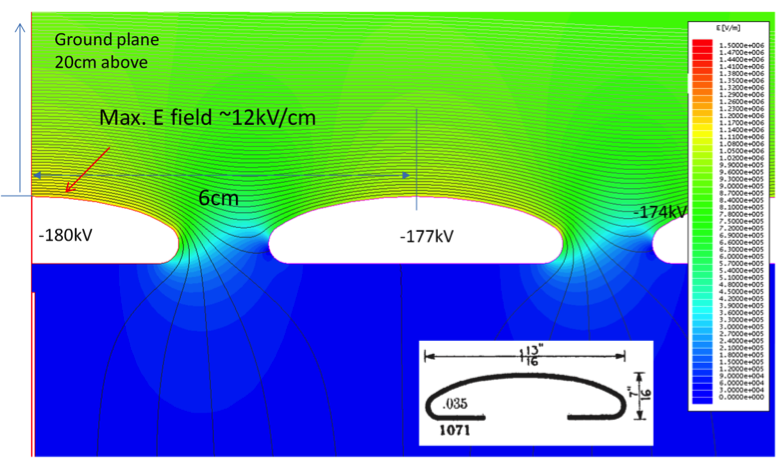
\includegraphics[width=0.8\textwidth]{profile-e-field.png}
\end{dunefigure}

The profiles ends are equipped with UHMW polyethylene caps to reduce the risk of arc formation.  These caps are designed to have sufficient wall thickness (\SI{6}{\milli\m}) to withstand the full voltage across their walls.

The aluminum profiles are attached to fiber-reinforced plastic (FRP) pultruded structural elements, including I-beams and box beams.  
Pultruded FRP material is non-conductive and strong enough to withstand the \dword{fc} loads  in the temperature range of \SI{-150}{C} and \SI{23}{C}, as certified by vendors. Testing of the FRP joints were conducted at liquid nitrogen temperatures (see DocDb 1504).  The strength of the material increased over room temperature tests which provides confidence in the material behavior at \lar  temperature. Tests of FRP joints at LN temperature\fixme{ add citations in bib: CPA and FC Design, DUNE DocDB 1504} showed that the strength of the material increases at cryogenic temperature relative to room temperature, providing confidence in FRP material behavior at LAr temperature.
%FRP has all of the reinforcing fibers running along the main axis of the section being used.  
The FRP material meets class A standards for fire and smoke development established by the International Building Code characterized by ASTM E84\footnote{\textit{Standard Test Method for Surface Burning Characteristics of Building Materials}, ASTM International, \url{https://compass.astm.org/EDIT/html_annot.cgi?E84+18}.}

As discussed in Section~\ref{sec:fdsp-hv-intro}, %the Introduction, 
the field cage modules are of two types: the top and bottom \dword{fc} and the \dword{ewfc}, both of which are described below. 
A resistive divider chain interconnects all the aluminum profiles to provide a linear voltage gradient between the cathode and anode planes.  The top and bottom modules are nominally \SI{2.3}{\m} wide by \SI{3.5}{\m} long. A \dword{gp}, in the form of tiled, perforated stainless steel sheet panels, is mounted on the outside surface of the T/B field cage module with a \SI{20}{\cm} clearance. The top and bottom \dword{fc} modules are supported by the \dwords{cpa} and \dwords{apa}. The \dword{ewfc} modules are \SI{1.5}{\m} tall by \SI{3.5}{\m} long. They are stacked eight units high (\SI{12}{\m}), and are supported by the installation rails above the \dwords{apa} and \dwords{cpa}.

The \dwords{fc} are designed to produce a uniform field with understood characteristics.
The current (i.e., \dword{pdsp}) \dword{fc} design has a large gap between the \dword{ewfc} module and its neighboring top and bottom modules to allow the latter to swing pass the \dword{ewfc} during the \dword{fc} deployment. This gap causes the largest known distortion in the drift field in the \dword{tpc}. Figure~\ref{fig:fc-distortion} shows the extent of the distortion in this limiting scenario. In \dword{pdsp}, the gap produces two regions (of total \lar mass \SI{20}{kg}) in the TPC near both bottom corners that suffer \SI{5}{\%} \efield distortions.

\begin{dunefigure}[Electric field at edge of \dword{fc}]
{fig:fc-distortion}
{\efield at a corner between the bottom and endwall \dword{fc} modules, showing effects of a \SI{7}{cm} gap. Left: the extent of \num{5}\% \efield{} non-uniformity boundary (black surface, contains less than \SI{10}{kg} of \lar) and \num{10}\% non-uniformity boundary (white surface, contains $\sim$ \SI{6}{kg} of \lar) inside the TPC's active volume. The inset is a view from the CAD model.  Right: electron drift lines originating from the cathode surface.}
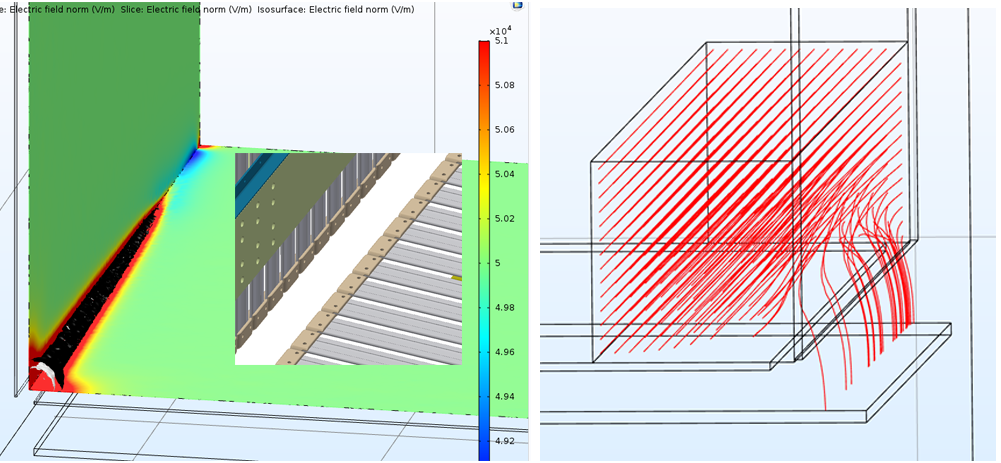
\includegraphics[width=0.9\textwidth]{distortion_from_fc_gap}
\end{dunefigure}

The \dwords{fc} %have been 
are designed to %ensure they 
meet the system requirements specified in Table~\ref{tab:hvphysicsreqs}. All components other than the aluminum profiles, \dwords{gp}, and electronic divider boards are made of insulating FRP and FR4 materials, and the end of each profile is covered with a UHMWPE end cap, to allow the system to reach the design \dword{tpc} \efield{} (requirement 1). The profiles have been carefully modeled to study the resulting \efield{}, and small-scale laboratory tests have been conducted to ensure that the maximum \efield{} does not approach \SI{30}{\kV\per\cm} (requirement 2). These design features are expected to avoid sparking, and thus to draw very small stable currents, which should produce a consistent load on the power supply (requirements 3, 4, and 5). Finally, all voltage divider boards provide redundant paths for establishing the profile-to-profile potential differences, and two redundant boards provide the connection from the \dwords{fc} modules to the \dword{cpa} (requirement 6).

%%%%%%%%%%%%%%%%%%%%%%%%%%%%%%%%%%%%%%%%%%%%%%
\subsubsection{Top and bottom field cages}

The \dword{topfc} and \dword{botfc} modules are \spfcmodlen{} long, which is set by the length of the two \SI{15.2}{\cm} (\SI{6}\,in) FRP I-beams that form the primary support structure of the modules. The I-beams are connected to each other by three  \SI{7.6}{\cm} (\SI{3}\,in) FRP cross beams. The connections between the longitudinal and cross I-beams are made with L-shaped FRP braces that are attached to the I-beams with FRP spacer tubes, and secured with FRP threaded rods, FRP hex-head nuts, and custom-machined FR4 washer plates.

The modules are \SI{2.3}{\m} wide, which corresponds to the length of the aluminum profiles, including the UHMW polyethylene end caps. Profiles are secured to the FRP frame using custom-machined double-holed stainless steel slip nuts that are slid into and electrically in direct contact with the Al profiles such that they straddle the webbing of the \SI{15}{\cm} I-beams, and are held in place with screws that penetrate the I-beam flanges. The profile offset with respect to the FRP frame is different for modules closest to the \dwords{ewfc}, %endwalls, 
and modules in the center of the active volume.

Each \dword{topfc} and \dword{botfc} module holds five ground planes, which are connected to the outside (i.e., the non-drift side) of the module. The \dwords{gp} are positioned $\sim$\SI{20.5}{\cm} above the profiles, and are pushed to the \dword{cpa} side of the module, leaving the last 14 profiles (\SI{88}{\cm}) on the \dword{apa} side of the module exposed. Between the \dwords{gp} and the \SI{15}{\cm} I-beams are standoffs made of short sections of \SI{10.2}{\cm} (4\,in)  FRP I-beams, which are connected with FRP threaded rods and slip nuts. The electrical connection between the ground planes is made with copper strips.

The connections between the top and bottom modules and the \dwords{cpa} are made with aluminum hinges, \SI{2.54}{\cm} (1\,in) in thickness, that allow the modules to be folded in to the \dword{cpa} during installation. The hinges are electrically connected to the second profile from the \dword{cpa}. The connections to the \dwords{apa} are made with stainless steel latches that are engaged once the top and bottom modules are unfolded and fully extended toward the \dword{apa}.

The voltage drop between adjacent profiles is established by voltage divider boards that are screwed into the drift volume side of the profiles. A custom-machined nut plate is used that can be inserted into the open slot of each profile and twisted \SI{90}{\degree} %$^\circ$ 
to lock into position. Two additional boards to connect the modules to the \dwords{cpa} were screwed into the last profile on the \dword{cpa}-side of the module. This system is also described in Section~\ref{sec:fdsp-hv-design-interconnect}. A fully assembled module is shown in Figure~\ref{fig:tbfc1-2}.

\begin{dunefigure}[Top and bottom field cage modules]{fig:tbfc1-2}{The fully assembled modules with ground planes are shown (left), as well as a close up of a \dword{cpa} end as viewed from the bottom (drift) side of the module.}
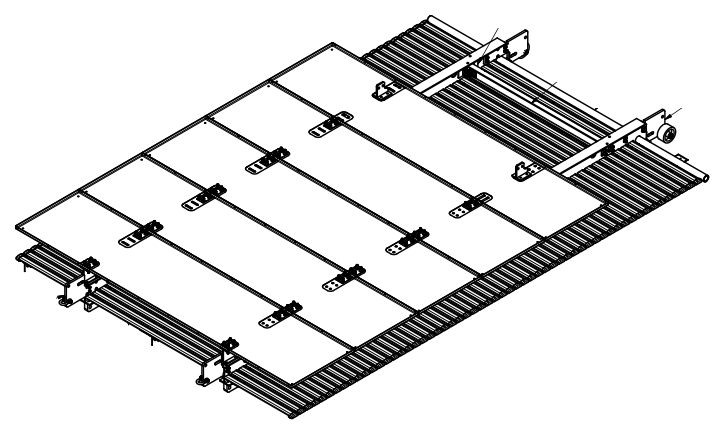
\includegraphics[width=0.65\textwidth]{tbfc1}
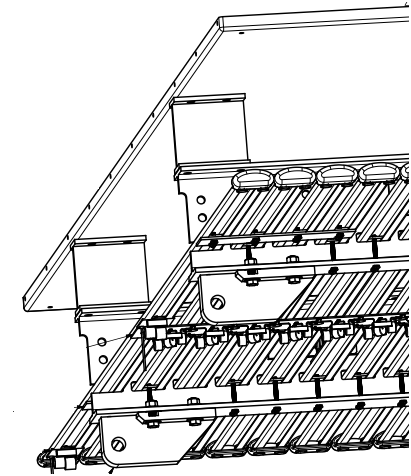
\includegraphics[width=0.33\textwidth]{tbfc2}
\end{dunefigure}

Between any two adjacent nodes of the resistor divider chain are two \SI{5}{\giga\ohm} resistors, and three serially connected metal oxide varistors (MOVs) in parallel.  The nominal voltage drop is \SI{3}{kV} between each node.
An open resistor on the divider chain would approximately double the voltage across the remaining resistor to \SI{6}{kV}.  This will force the varistors in parallel to that resistor into conduction mode, resulting in a voltage drop of roughly \SI{5}{kV} (\SI{1.7}{kV} $\times$ \num{3}), while the rest of the divider chain remains linear, with a slightly lower voltage gradient.
Because the damage to the divider would be local to one module, its impact to the \dword{tpc} drift field is limited to region near this module.  This is part of the intention of the modular design.
An example of a simulated \efield{} distortion which would be caused by a failed resistor is shown in Figure~\ref{fig:fc-broken-resistor}. 

\begin{dunefigure}[\efield distortion from broken voltage divider path]{fig:fc-broken-resistor}{Simulated \efield{} distortion from one broken resistor in the middle of the voltage divider chain on one bottom field cage module, emphasizing the need for redundancy. Left: Extent of \efield{} non-uniformity in the active volume of the TPC. the green planes mark the boundaries of the active volume inside the field cage. The partial contour surfaces represent the volume boundaries where \efield{} exceeds 5\% (dark red, contains less than 100\,kg of LAr) and 10\% (dark blue, contains less than 20\,kg of LAr) of the nominal drift field. Units are \si{\volt\per\m} in the legend. Right: electron drift lines connecting the \dword{cpa} to \dword{apa} in a bottom/end wall field cage corner.  The maximum distortion to the field line is about 5\,cm for electrons starting at mid drift at the bottom edge of the active volume.}
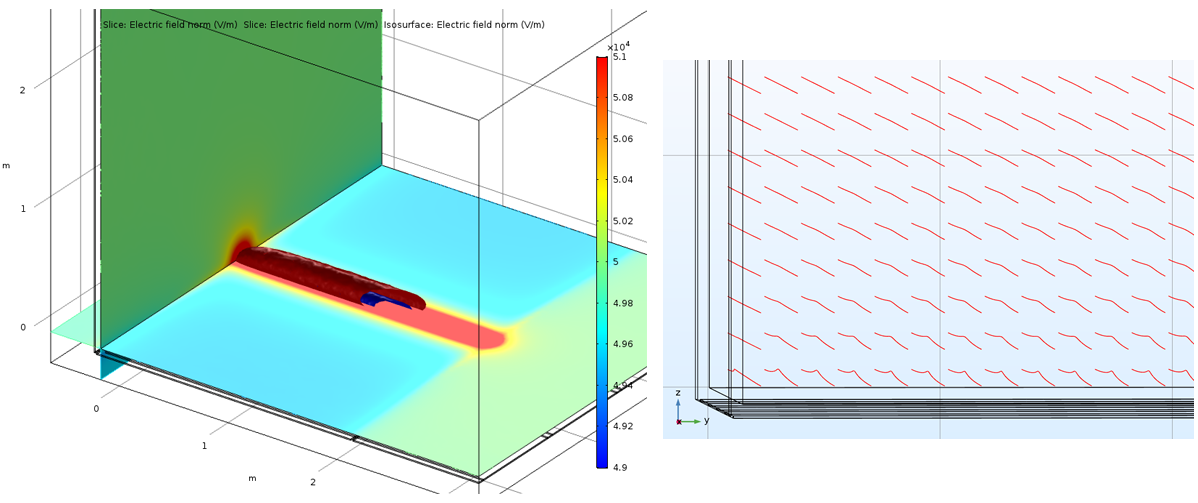
\includegraphics[width=0.9\textwidth]{e-field-distortion-due-to-open-resistor}
\end{dunefigure}
The effect of the non-uniformity in resistor values can also be scaled from this study.  A 2\% change in a resistor value (1\% change from the 2R in parallel) would give about 1.5\% of the distortion from a broken resistor, i.e. less than 1\,mm of transverse distortion in track position, with no noticeable drift field amplitude change inside the active volume.
 

\subsubsection{Endwall field cages (EWFC)}

%The endwall field cage (\dword{ewfc}) for each of the four drift volumes consists of two endwalls (EW), one on each side of the drift volume. Each endwall is in turn composed of eight endwall modules (EW-Modules). 

Each of the four drift volumes has two \dwords{ewfc}, one on each end. Each \dword{ewfc} is in turn composed of eight \dword{ewfc} modules.
There are two different types of \dword{ewfc} modules, each of which comes in a \textit{regular} and in a \textit{mirrored} configuration to account for 
mounting constraints and to match the detector geometry. Figure~\ref{fig:fc_endwall_panels} illustrates the layout for the topmost 
and the other panels, respectively.

\begin{dunefigure}[Endwall \dword{fc} panels]{fig:fc_endwall_panels}{Left: Uppermost panel of the \dword{ewfc}. Right: Non-uppermost \dword{ewfc} panel.}
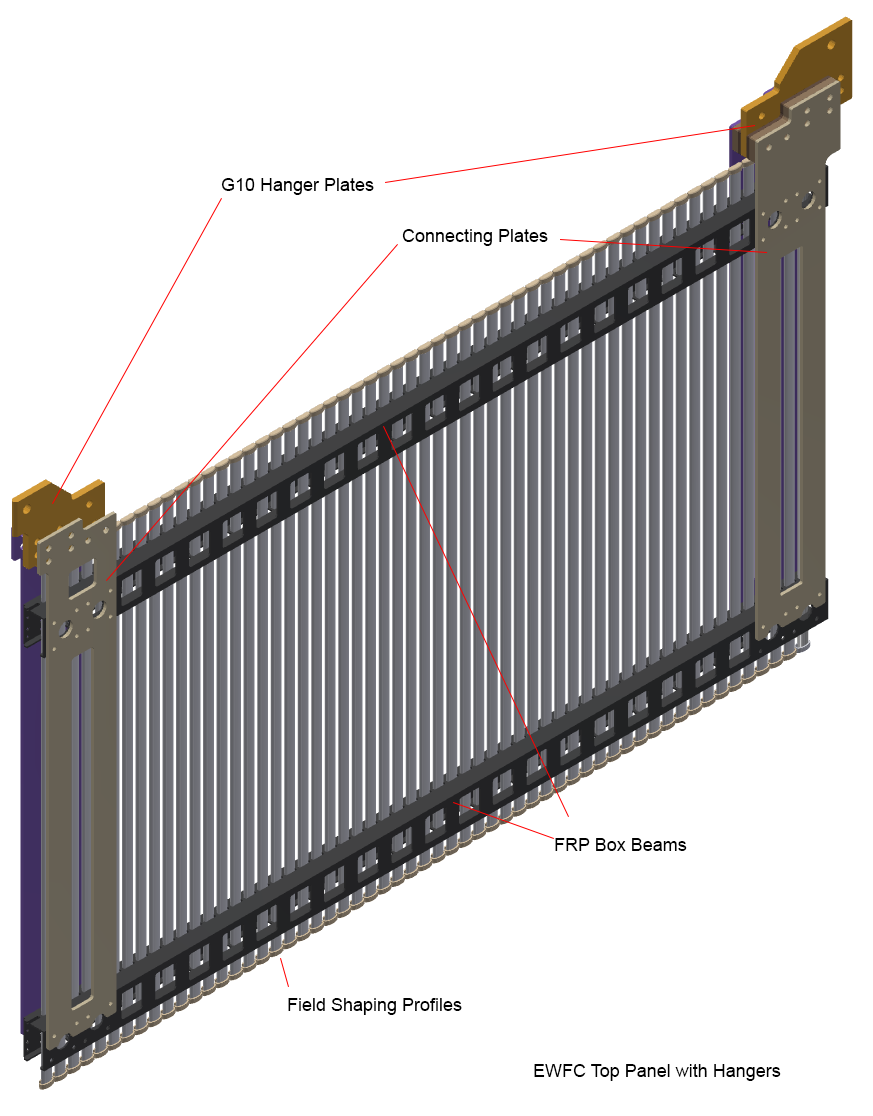
\includegraphics[width=0.48\textwidth]
{EWFC_Top_Module}
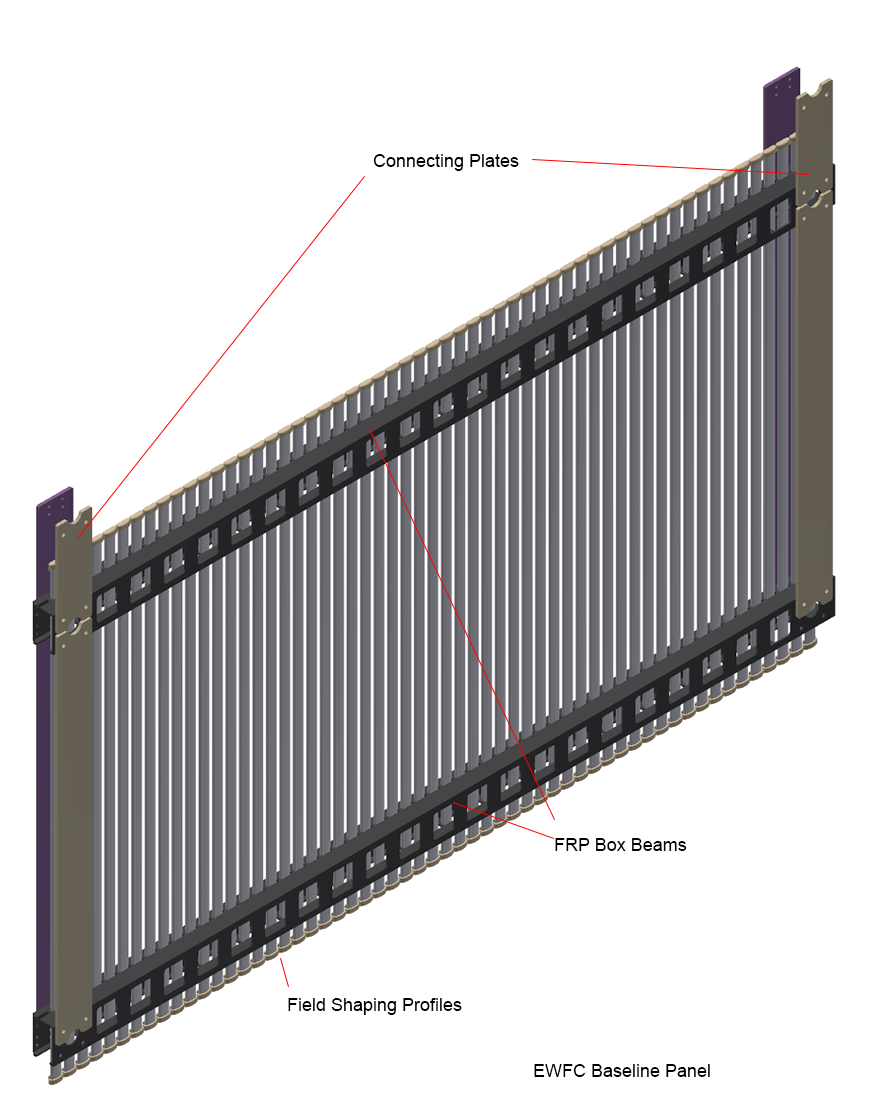
\includegraphics[width=0.48\textwidth]
{EWFC_Baseline_Module}
\end{dunefigure}

Each \dword{ewfc} module is constructed of two FRP box beams which are \SI{3.5}{\m} long. The box beam design also incorporates cutouts on the outside face to minimize charge build up. Box beams are connected using \SI{1.27}{\cm} (\num{0.5}\,in) thick FRP plates. The plates are connected to the box beams using a shear pin and bolt arrangement. The inside plates facing the active volume are connected using special stainless steel slip nuts and stainless steel bolts. The field-shaping profiles are connected to the top box beam using stainless steel slip nuts, an FRP angle, and two screws each. The profiles are connected to the bottom box beam with a slip nut that is held in place by friction.

%\begin{center}
%   \parbox[t]{0.47\textwidth}{
 %  \resizebox{0.47\textwidth}{!}{\includegraphics[width=0.48\textwidth]{\dword{fc}endwall_top-panel.png}}
%\caption{\label{fig:\dword{fc}endwall_top} Uppermost panel of the field cage endwall. {\color{red} NOTE: need to replace figure with updated version for DUNE, e.g. without middle FRP cross member.}}}
%\makebox[0.025\textwidth]{}
 %  \parbox[t]{0.48\textwidth}{
 %  \resizebox{.48\textwidth}{!}{\includegraphics[width=0.48\textwidth]{\dword{fc}endwall_panel.png}}
%\caption{\label{fig:\dword{fc}endwall_panel} Baseline field cage panel. {\color{red}NOTE: need to replace figure with updated version for DUNE, e.g. without middle FRP cross member.}}}
%\end{center}


\subsection{Electrical Interconnections} % (Glenn)
\label{sec:fdsp-hv-design-interconnect}

\begin{dunefigure}[\dword{hv} interconnection topology]{fig:fdsp-hv-design-interconnect-concept}
  {High-level topology of the \dword{hv} interconnections}
  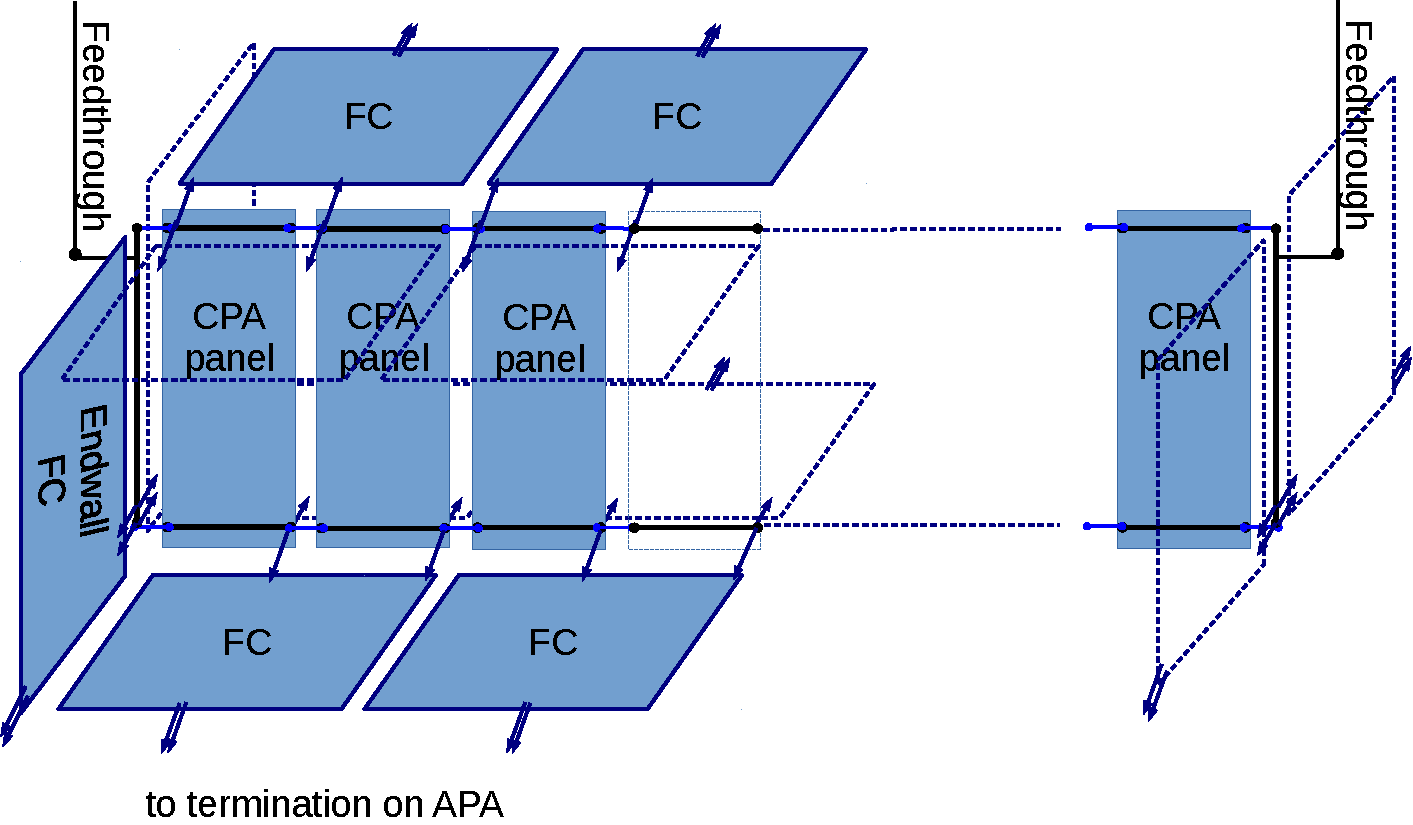
\includegraphics[width=0.7\textwidth]{fdsp-hv-interconnection-topology}
\end{dunefigure}

Electrical interconnections are needed among the \dword{hv} delivery system, \dword{cpa} planes, \dword{fc} modules, and termination
boards on the \dword{apa} modules, as well as between resistive dividers and
the field-forming elements on the \dwords{cpa} and \dwords{fc}.  Redundancy is
needed to avoid single points of failure. 
Some connections must be
insulated in order to avoid creating a discharge path that might
circumvent the discharge mitigation provided by the resistive \dword{cpa}
surface and \dword{fc} partitioning.  Certain connections must be
flexible in order to allow for \dword{fc} deployment, thermal
contraction, and motion between separately supported \dwords{cpa}.  Figure~\ref{fig:fdsp-hv-design-interconnect-concept} shows a high-level
overview of the interconnections between the \dword{hv}, \dword{cpa}, and \dword{fc} modules.


%% connections between major elements (\dword{hv}, \dword{cpa}, \dword{fc}, \dword{apa})
High voltage feedthroughs connect to cups mounted on the \dword{cpa} frame
%\cite the \dword{hv} delivery section
that attach to a \dword{hv} bus running through the \dwords{cpa}.  \Dword{hv} bus connections
between \dword{cpa} panels are made by flexible wires through holes in the
\dword{cpa} frame. The \dword{hv} bus is a loop in order to mitigate risk of a single
point failure; feedthroughs at each end of each \dword{cpa} plane mitigate
risk of a double-break failure.  Voltage dividers on each \dword{cpa} panel
bias the field shaping strips and the resistive dividers on the top
and bottom \dwords{fc}.  \dword{cpa}-to-\dword{fc} connections are made using
flexible wire to accommodate \dword{fc} deployment.  To further
increase redundancy, two \dword{cpa} panels connect to each top or bottom
field cage, and two connections are also made to each \dword{ewfc}. Resistor divider boards attach directly to the interior side of
the \dword{fc} profiles with screws.   A redundant pair of flexible wires
connects a circuit board on the last profile of each \dword{fc} to a
bias-and-monitoring board mounted on the corresponding \dword{apa}.

%% connections within \dword{cpa}
Short sections of flexible wire at the ends of each \dword{hv} bus segment
attach to screws in brass tabs on the \dword{cpa} resistive panels (\dword{cpa} RPs).
%\cite \dword{cpa} design subsection
Vertical \dword{hv} bus segments on the outer ends of each \dword{cpa} plane connect
the top and bottom \dword{hv} buses to complete the loop.  Solid wire is used
to connect resistive panels within a \dword{cpa} panel.

%% \dword{fc} connections
Each \dword{fc} module is as electrically independent as possible in order to
mitigate discharge.  However, only the bottom module of each endwall
can make connections to the \dword{hv} bus and \dword{apa}, so each endwall module
is connected to its upper neighbor at its first and last profiles
using metal strips.

%% Regarding wire terminals and screws
All flexible wires have ring or spade terminals and are secured by
screws in brass tabs.  Spring washers are used with every electrical
screw connection in order to maintain good electrical contact with
motion and changes of temperature.

Table \ref{tab:sp-hv-interconnects} summarizes the interconnections
required.

\begin{dunetable}
[\dword{hv} system interconnections]
{p{0.35\linewidth}p{0.62\linewidth}}
{tab:sp-hv-interconnects}
{\dword{hv} System Interconnections}   
 Connection & Method \\ \toprowrule
 \dword{hv} cup to \dword{hv} bus & wire to screw in \dword{hv} cup mount on \dword{cpa} frame \\
 \dword{hv} bus between \dword{cpa} panels & wire between screws in brass tabs \\
 \dword{hv} bus to \dword{fss} & wire to circuit board mounted on \dword{fss} \\
 \dword{fss} to \dword{topfc} and \dword{botfc} & wire to circuit board on first \dword{fc} profile, two per \dword{fc} module \\
 \dword{hv} bus to endwall \dword{fc} & wire to circuit board mounted on first \dword{fc} profile, two per endwall \\
 \dword{fc} divider circuit boards & directly attached to profiles using screws \\
 \dword{fc} to bias and monitoring termination & redundant wires from board mounted on last \dword{fc} profile \\
 \dword{hv} bus to \dword{cpa} panels & brass tab on \dword{cpa} resistive panel \\
 \dword{cpa} RP interconnections & solid wire between screws in brass tabs \\
 Endwall \dword{fc} module interconnections & metal strips, first and last profiles only
 \\
\end{dunetable}

The redundancy in electrical connections described above meets requirement (6).
The \dword{hv} bus and interconnections are all made in low field regions in order to meet requirement (2).
The \dword{hv} bus cable is rated at the full cathode \dword{hv} such that even in case of a rapid discharge of the \dword{hv} system no current can flow to the cathode or \dword{fc} except at the intended contact points, preserving the ability of the resistive cathode and \dwords{fc} to meet requirement (5).

%%%%%%%%%%%%%%%%%%%%%%%%%%%%%%%%%%%
%\subsection{Quality Assurance}
%\label{sec:fdsp-hv-qa}


%%%%%%%%%%%%%%%%%%%%%%%%%%%%%%%%%%%%%%%%%%%%%%%%%%%%%%%%%%%%%%%%%%%%
\section{Production and Assembly}
\label{sec:fdsp-hv-prod-assy}

%%%%%%%%%%%%%%%%%%%%%%%%%%%%%%%%%%
\subsection{Power Supplies and Feedthroughs}
\label{sec:fdsp-hv-supplies-feedthroughs}

Power supplies will be commercially procured, for example through Heinzinger. The \dword{hv} cable is commercially available.

The power supply is tested extensively along with the controls and monitoring software.  Features to be included in the software are:
\begin{itemize}
\item The ability to ramp, or change the voltage.  The rate and an ability to pause the ramp shall be included.  In previous installations, the ramp rate was typically between 60 to 120 V/s.
\item An input for a user-defined current limit.  This parameter is the current value at which the supply reduces the voltage output to stay below the current limit.  The current-limiting is done in hardware.
\item An input for a trip threshold.  At this current reading, the program would reduce the voltage output through software.  In previous experiments, the trip function in software would set the output to \SI{0}{kV}.
\end{itemize}
\noindent Additionally, the software should record the current and voltage read-back values with a user-defined frequency, as well as any irregular current or voltage events.

The \dword{hv} feedthroughs, filters, and splitter are custom devices.  One feedthrough option is to use the \dword{pdsp} design and similar procurement.  \Dword{hv} splitters are already on hand if they are desired.

%%%%%%%%%%%%%%%%%%%%%%%%%%%%%%%%%%
\subsection{Cathode Plane Assemblies}
\label{sec:fdsp-hv-prod-cpa}

The component parts of the \dword{cpa} %assembly 
are produced by commercial vendors for the following items:
%\fixme{clearly define cpa vs assembly, mentioned earlier}
\begin{itemize}
\item manufactured FR4 RP frames packed into three \dword{cpa} unit kits making up a \dword{cpa} panel,
\item carbon-impregnated Kapton coated resistive panels (RPs) and \dword{fss},
\item \dword{hv} cable segments and wire jumpers making up the \dword{cpa} \dword{hv} bus and RP interconnects,
\item machined brass tabs for connecting RPs, \dword{hv} Bus, and \dword{fss}, and
\item top, bottom, and exterior edge profiles and associated connection hardware.
\end{itemize}
The above items are packaged into \dword{cpa} panel kits by the vendors and are sent to the assembly factories, the locations of which will be determined later.  The basic construction unit for an assembly factory is a pair of \dword{cpa} panels so that shipment to \surf from an assembly factory consists of two \dword{cpa} panels that are paired on site to form a \dword{cpa} plane.

The most basic element of the \dword{cpa} is an RP mounted in a machined slot in the top, bottom and sides of FR4 frames.  There are three different types of these \dword{cpa} RP elements -- an upper, which has as its top frame the \dword{cpa} mounting bracket and \dword{topfc} hinge, a middle, and a lower, which has as its bottom frame a \dword{botfc} hinge.  Two such \dword{cpa} RP elements are bolted together and pinned to form a shipment \dword{cpa} unit of size \SI{1.2}{\m} $\times$ \SI{4}{\m}.  These \dword{cpa} units are assembled horizontally on a smooth, flat table to meet the dimensional requirements of \dword{cpa} construction.  In addition to the frames and RPs, %\dword{fss}s 
\dword{fss} strips are mounted on the exposed sides of the FR4 frames, aluminum profiles are attached to the top and bottom of the upper and lower elements, and cables are attached to the RPs to form segments of the \dword{hv} bus.  The shipment \dword{cpa} unit comes in three varieties in order to make a full \SI{12}{\m} tall \dword{cpa} Panel.  These are : (1) an upper \dword{cpa} RP element attached to a middle element, (2) two middle elements connected, and (3) a middle element attached to a lower element.  The \dword{cpa} unit order in the shipping crate from top to bottom is middle-and-lower, middle-and-middle, and upper-and-middle.  For the \SI{10}{\kt} \dword{spmod}, there are 100 upper elements, 100 lower elements and 400 middle elements that make up the 100 \dword{cpa} panels of the \dword{tpc}.
A comparison of a \SI{6}{\m} \dword{pdsp} \dword{cpa} panel and a \SI{12}{\m} \dword{pdsp} panel is shown at Ash River Laboratory in Minnesota, USA,  in Figure~\ref{fig:12m-cpa}.

\begin{dunefigure}[\dwords{cpa} at Ash River]{fig:12m-cpa}{A \SI{12}{\m} \dword{pdsp} \dword{cpa} panel and a smaller \SI{6}{\m}  panel mockup at Ash River.}  %closest panel 6m, each strip separated by 2m, this image taken in the pit at Ash River (where NOvA modules were stacked/glued.)
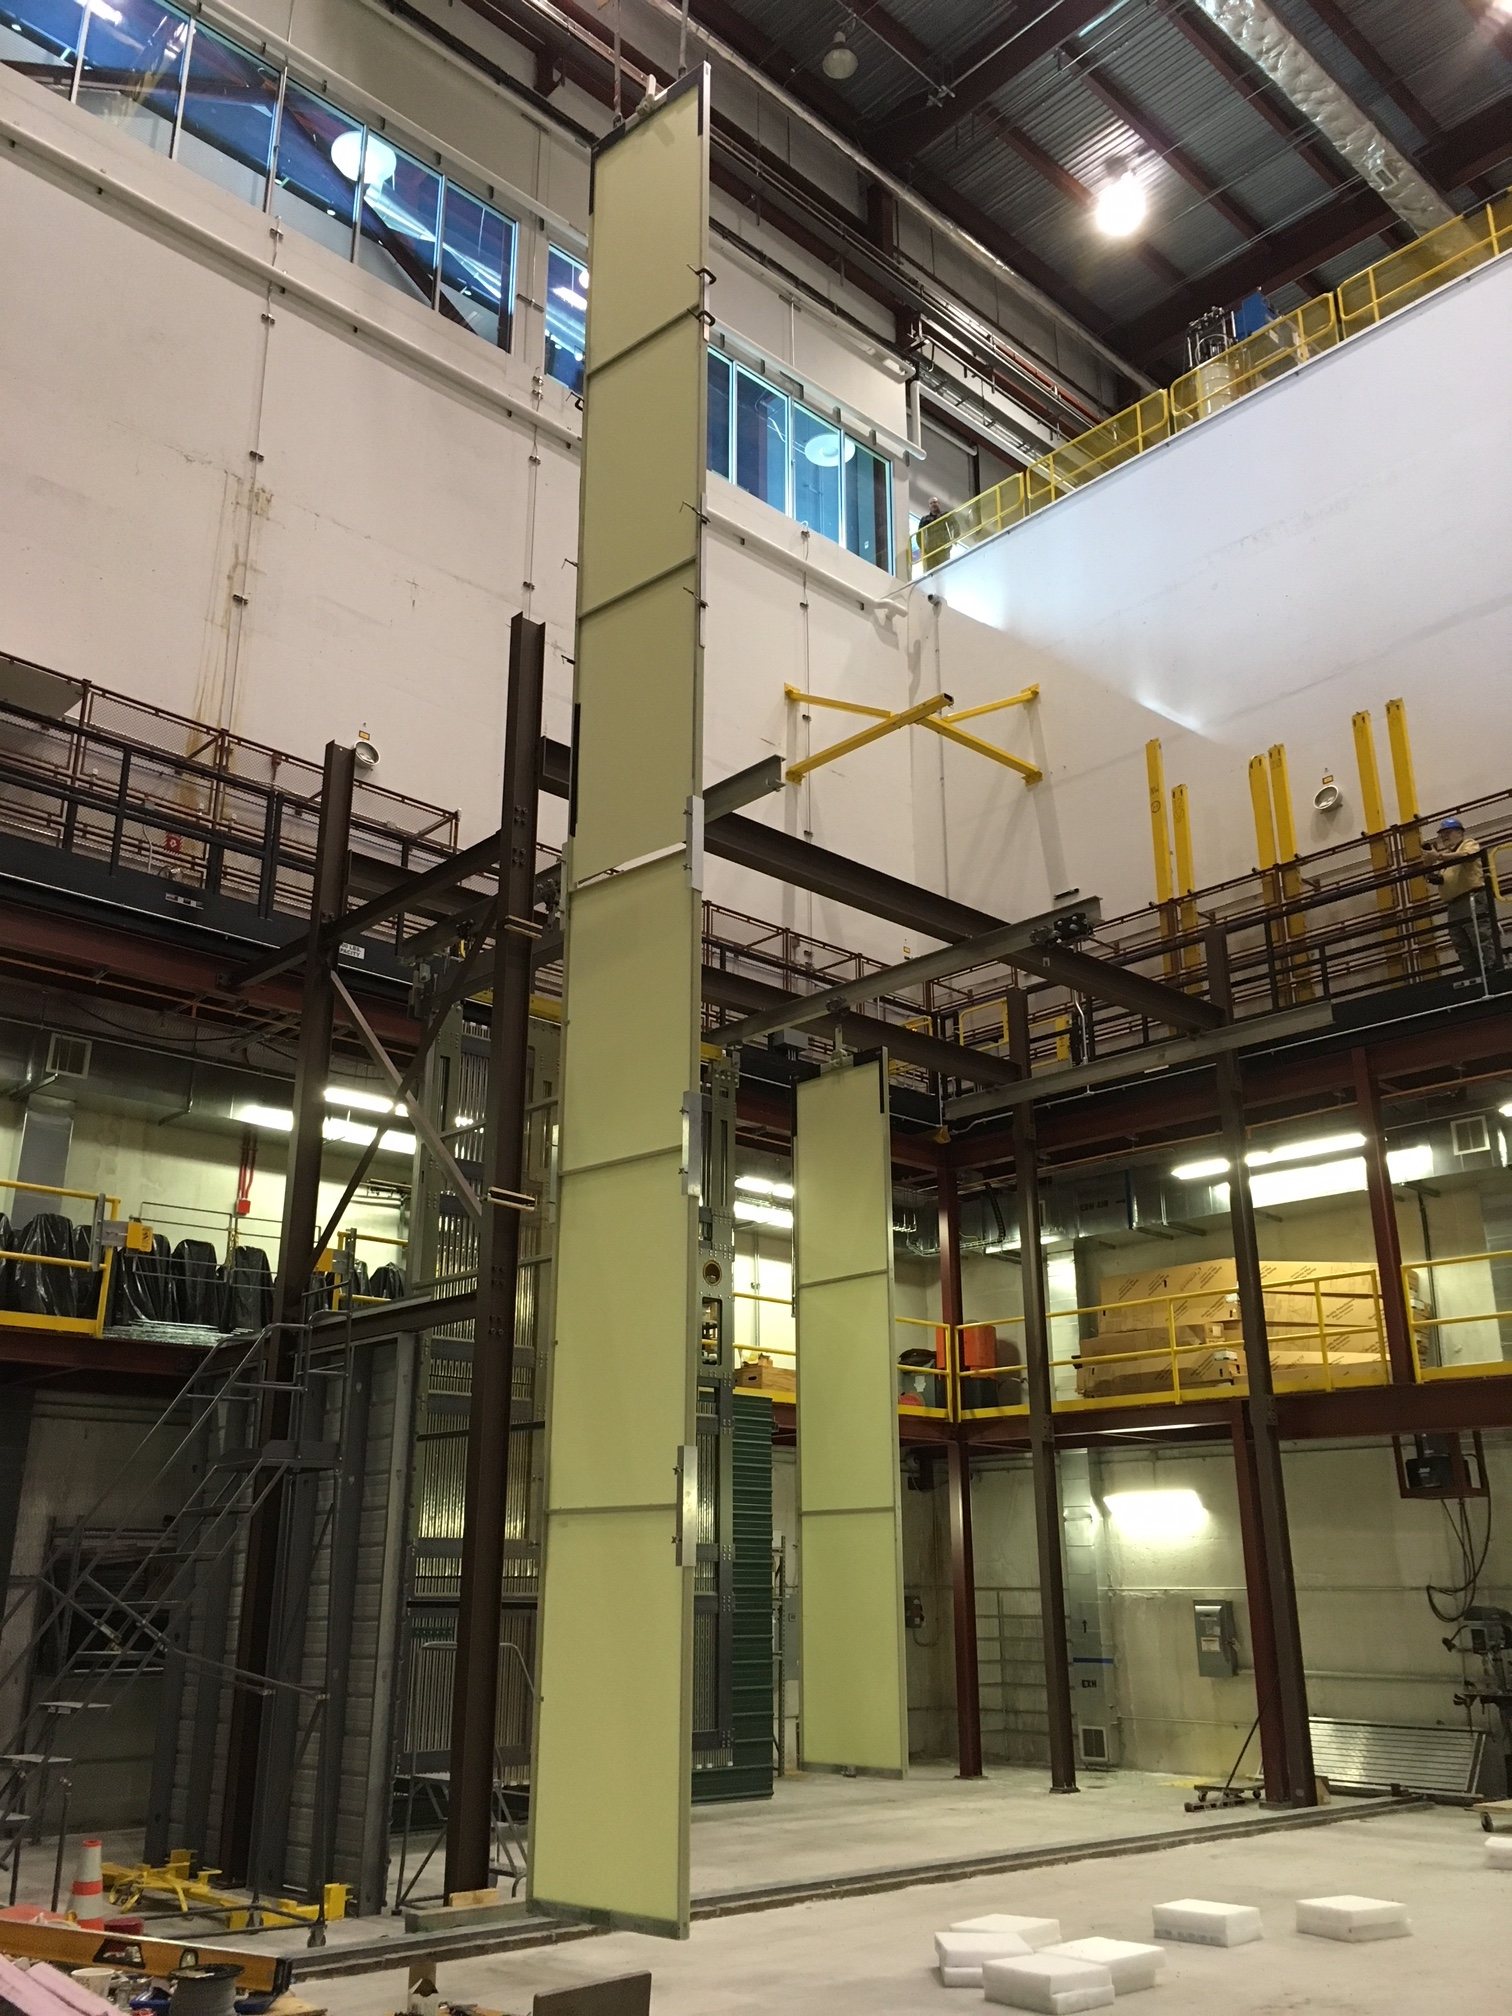
\includegraphics[width=0.35\textwidth]{12m-cpa}
\end{dunefigure}

\subsection{Field Cages}
\label{sec:fdsp-hv-prod-fc}

% Include profile procurement & QC here

\subsubsection{Top and Bottom Field Cages}

%Discussion of parts procurement, assembly, and testing.
The FRP and FR4 components of the  \dwords{topfc} and \dwords{botfc} will be commercially produced by firms that specialize in the machining of fiberglass components for electrical applications, as was successfully done for \dword{pdsp}. All parts are machined in the absence of water and cleaned with a lacquer thinner. Machined edges, other than small circular holes, are coated with translucent epoxy. The stainless steel and aluminum components will be produced in local university and commercial machine shops. Voltage divider boards and \dword{fc} and \dword{cpa} connection boards will likely be fabricated by university groups.
%The voltage divider boards will be provided by Louisiana State University, and the boards used to make the \dword{fc}/\dword{cpa} connection will be provided by Kansas State University.

The FRP frame assembly primarily consists of fastening together FRP I-beams with FRP threaded rods and hex nuts, which are secured with a limited and specified torque, to avoid damage to the threads. A detailed view of one of these connections is shown in Figure~\ref{fig:tbfc3}.

\begin{dunefigure}[Top and bottom \dword{fc} module frame assembly]{fig:tbfc3}{The above figure shows the procedure for connecting the cross beams to the main I-beams for the \dword{topfc}. Left: The components of each connection, which (from top to bottom) are the threaded rods, the spacer tubes, washer plates, the hexagonal nuts, and an L-shaped FRP brace. An intermediate stage (middle) and final stage (right) of the assembly are also shown."}
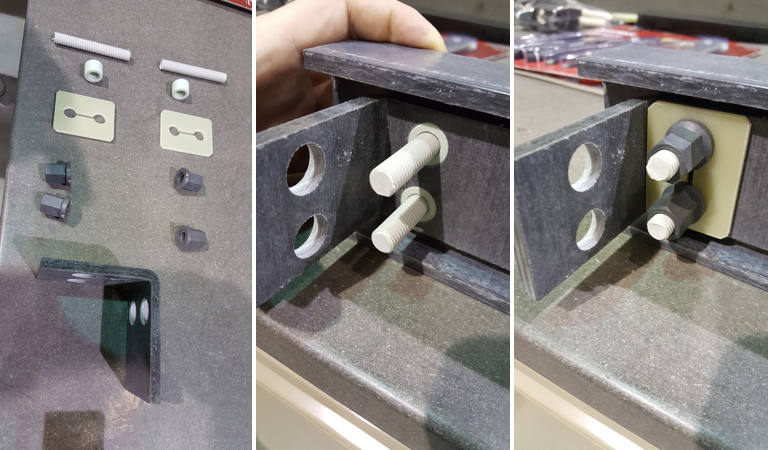
\includegraphics[width=0.70\textwidth]{tbfc3}
\end{dunefigure}

Prior to sliding each profile into the FRP frame, the holes should be covered with Kapton tape to avoid damage to the profile coating. An end cap is attached to each profile using plastic rivets, and then the profiles are aligned against an aligment fixture running the length of the \dword{fc}. After securing each profile to the frame, the tension in the mounting screws is adjusted to remove any angular deflection in the extended portion of the profile.

The ground planes are attached to the 10 cm stand-off I-beam sections with threaded rods and a machined plate. The copper strips are connected to adjacent modules at the same locations. Care must be taken to avoid bending the corners of the \dwords{gp} toward the profiles, particularly on the \dword{cpa} side of of the module.


\subsubsection{Endwall Field Cages}

All FRP plates are commercially cut to shape by water jet. The cut outs in the FRP box beams are also cut by water jet. Holes that accommodate G10 bushings are reamed in a machine shop. FRP frames are pre-assembled to ensure proper alignment of all FRP parts and matching of holes. The profiles are not inserted at this stage. The FRP modules are hung off of each other by means of interconnecting FRP plates to ensure accurate alignment.

Next, parts are labeled and the frames are taken apart. All components are cleaned by pressure washing or ultrasonic bath. All cut FRP surfaces are then coated with polyurethane, which contains the same main ingredient as the FRP resin, allowing it to bond well to the FRP fibers. Final panels are constructed from cleaned and inspected parts. In order to ease assembly, which requires access to both sides of a module,
a dedicated assembly table has been manufactured that allows convenient module rotation. 

Figure~\ref{fig:endwall_assy_rot_table} shows a partially assembled \dword{ewfc} FRP frame on the assembly table.
\begin{dunefigure}[Endwall assembly table]{fig:endwall_assy_rot_table}{Assembly table with partially assembled \dword{ewfc} module (Credit: LSU)}
 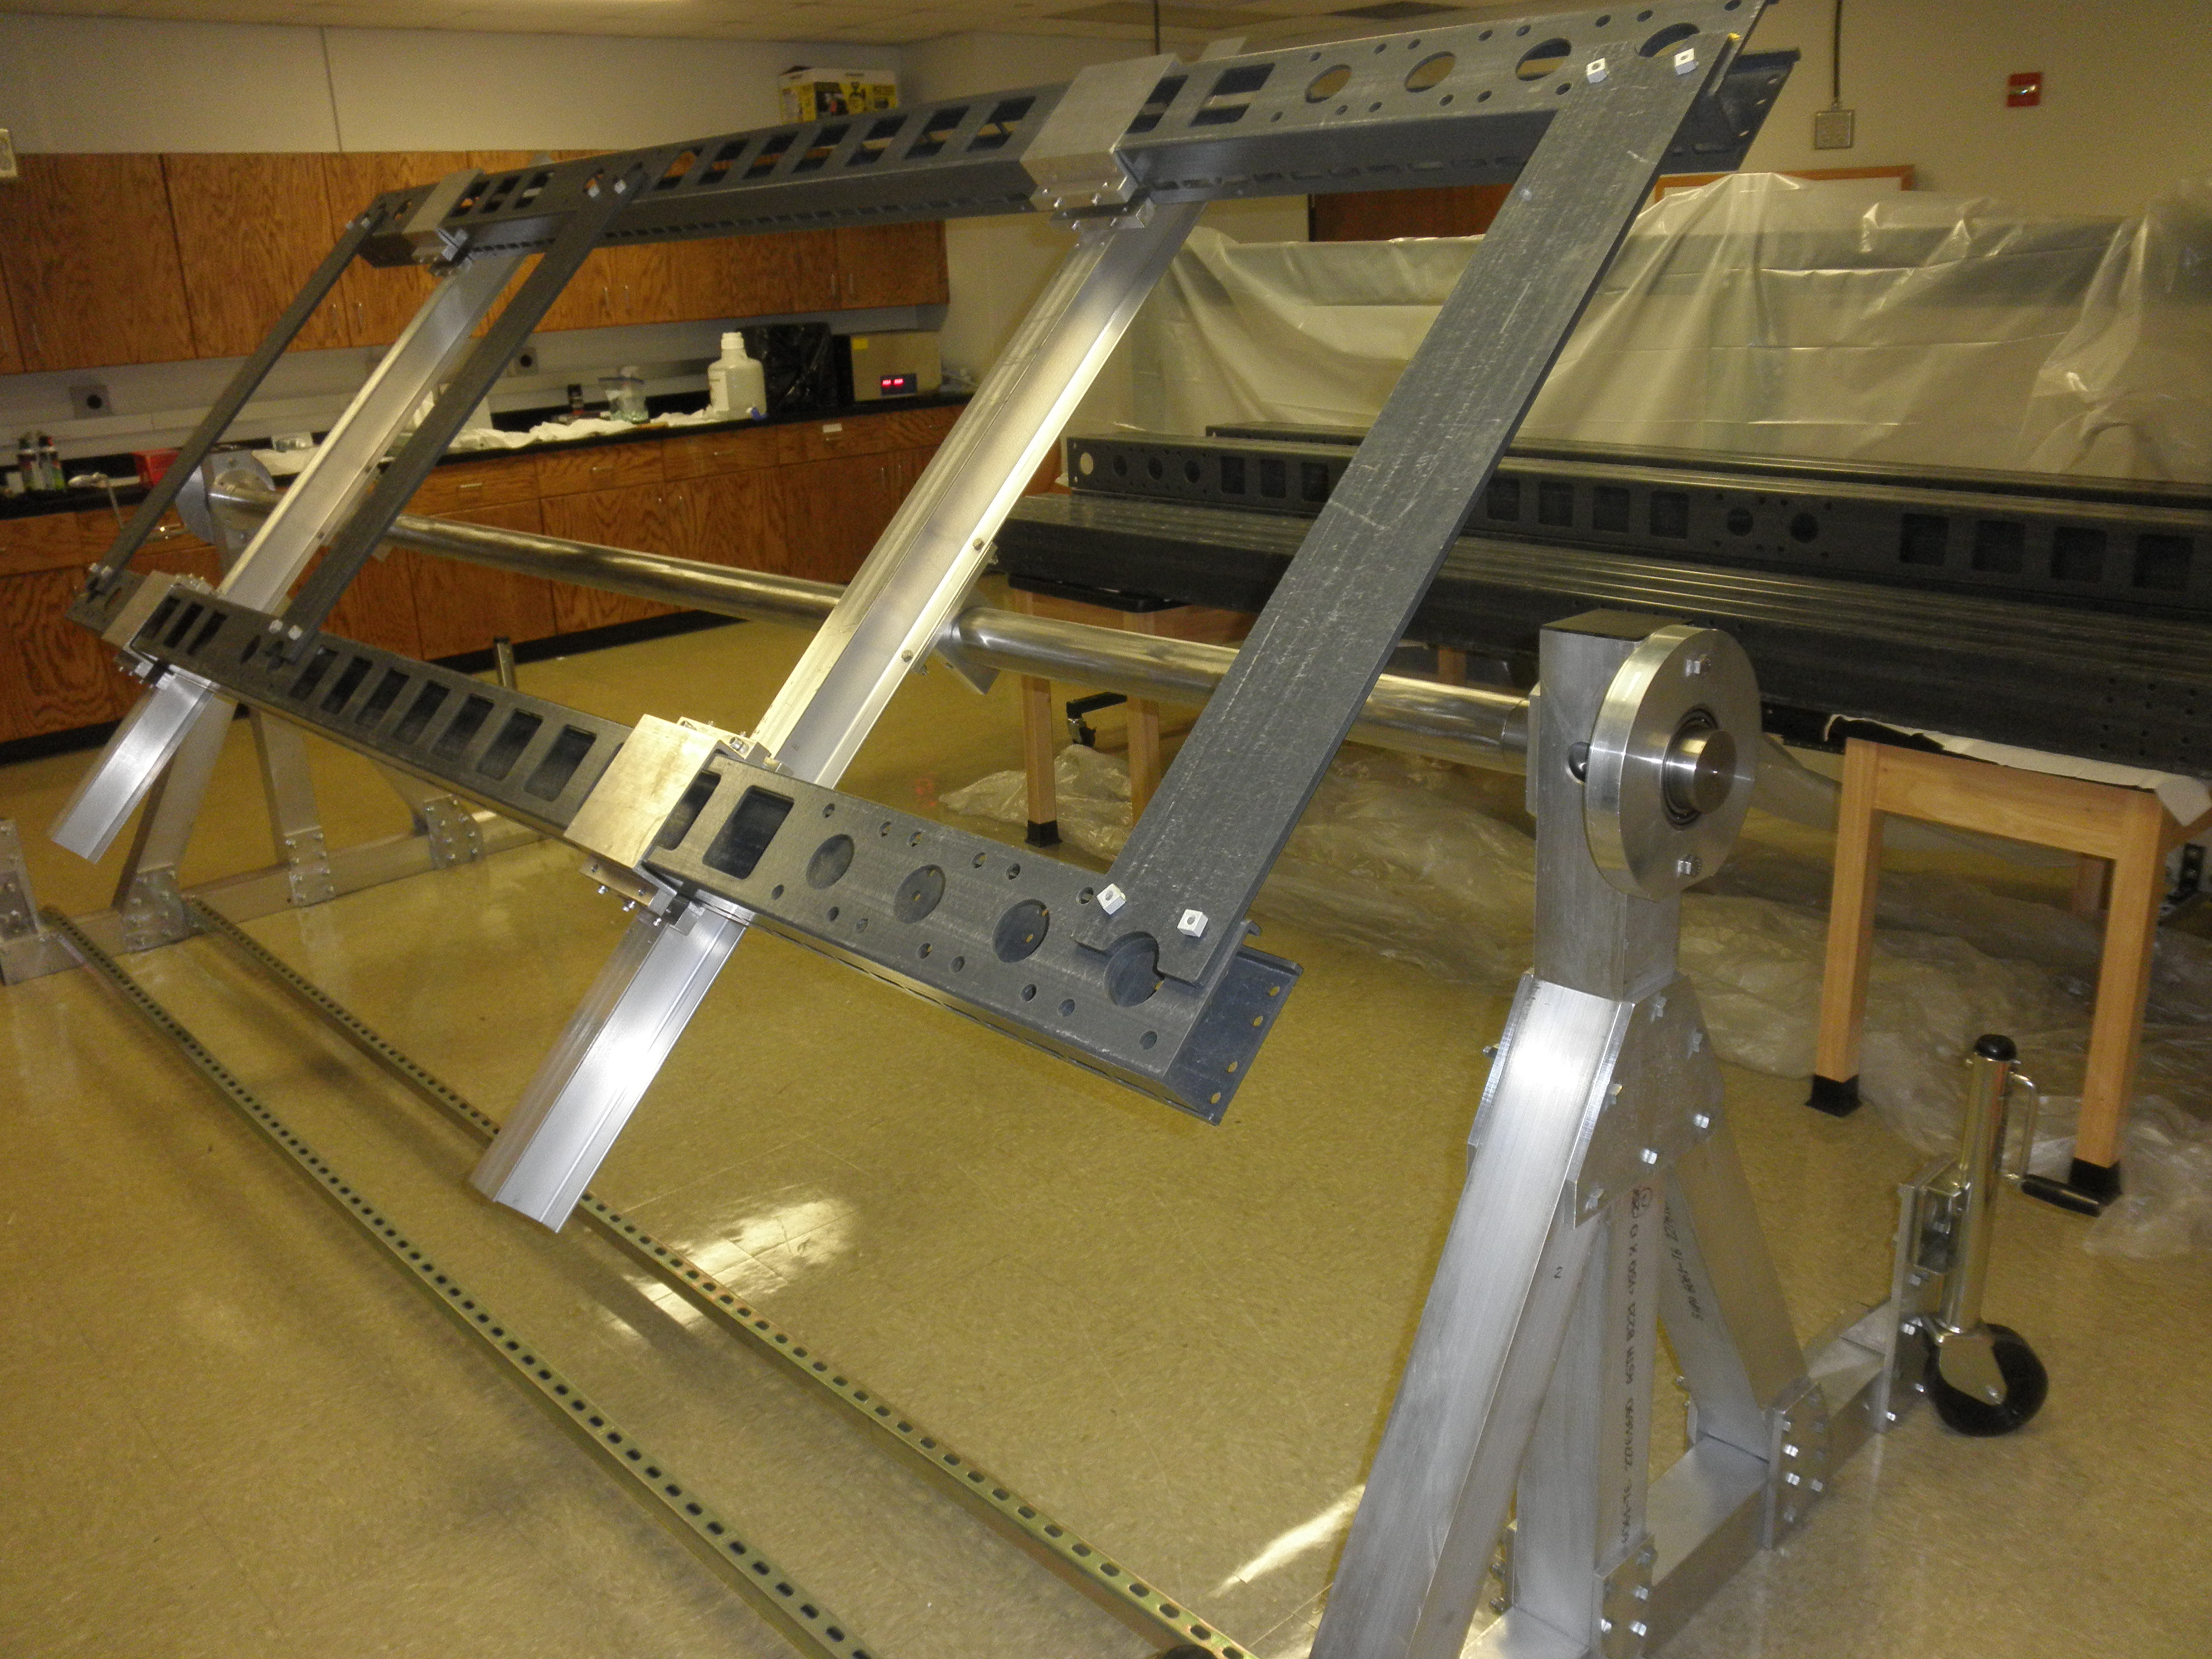
\includegraphics[width=0.8\textwidth]{endwall_assy_rot_table}
 \end{dunefigure}


The FRP box beams are sandwiched between \SI{1.27}{\cm} (\num{0.5}\,in) thick FRP panels which are held on one side by means of G10 bushings and rods with square nuts
as shown in Figure \ref{fig:endwall_assy_detail}. One the other side M10 stainless steel bolts engage with large slip nuts that are inserted into the Al profiles. The profiles 
are pulled towards a \SI{2.5}{\cm} thick FRP plate (red in Figure~\ref{fig:endwall_assy_detail}) on the inside of the box beam.
%

\begin{dunefigure}[Endwall assembly detail]{fig:endwall_assy_detail}{%Left: Side view of upper part of a top \dword{ewfc}  module.
Top and center \dword{ewfc} module frames hanging. (Credit: LSU)}
%\includegraphics[width=0.48\textwidth]
%{fc_endwall_detail_side}
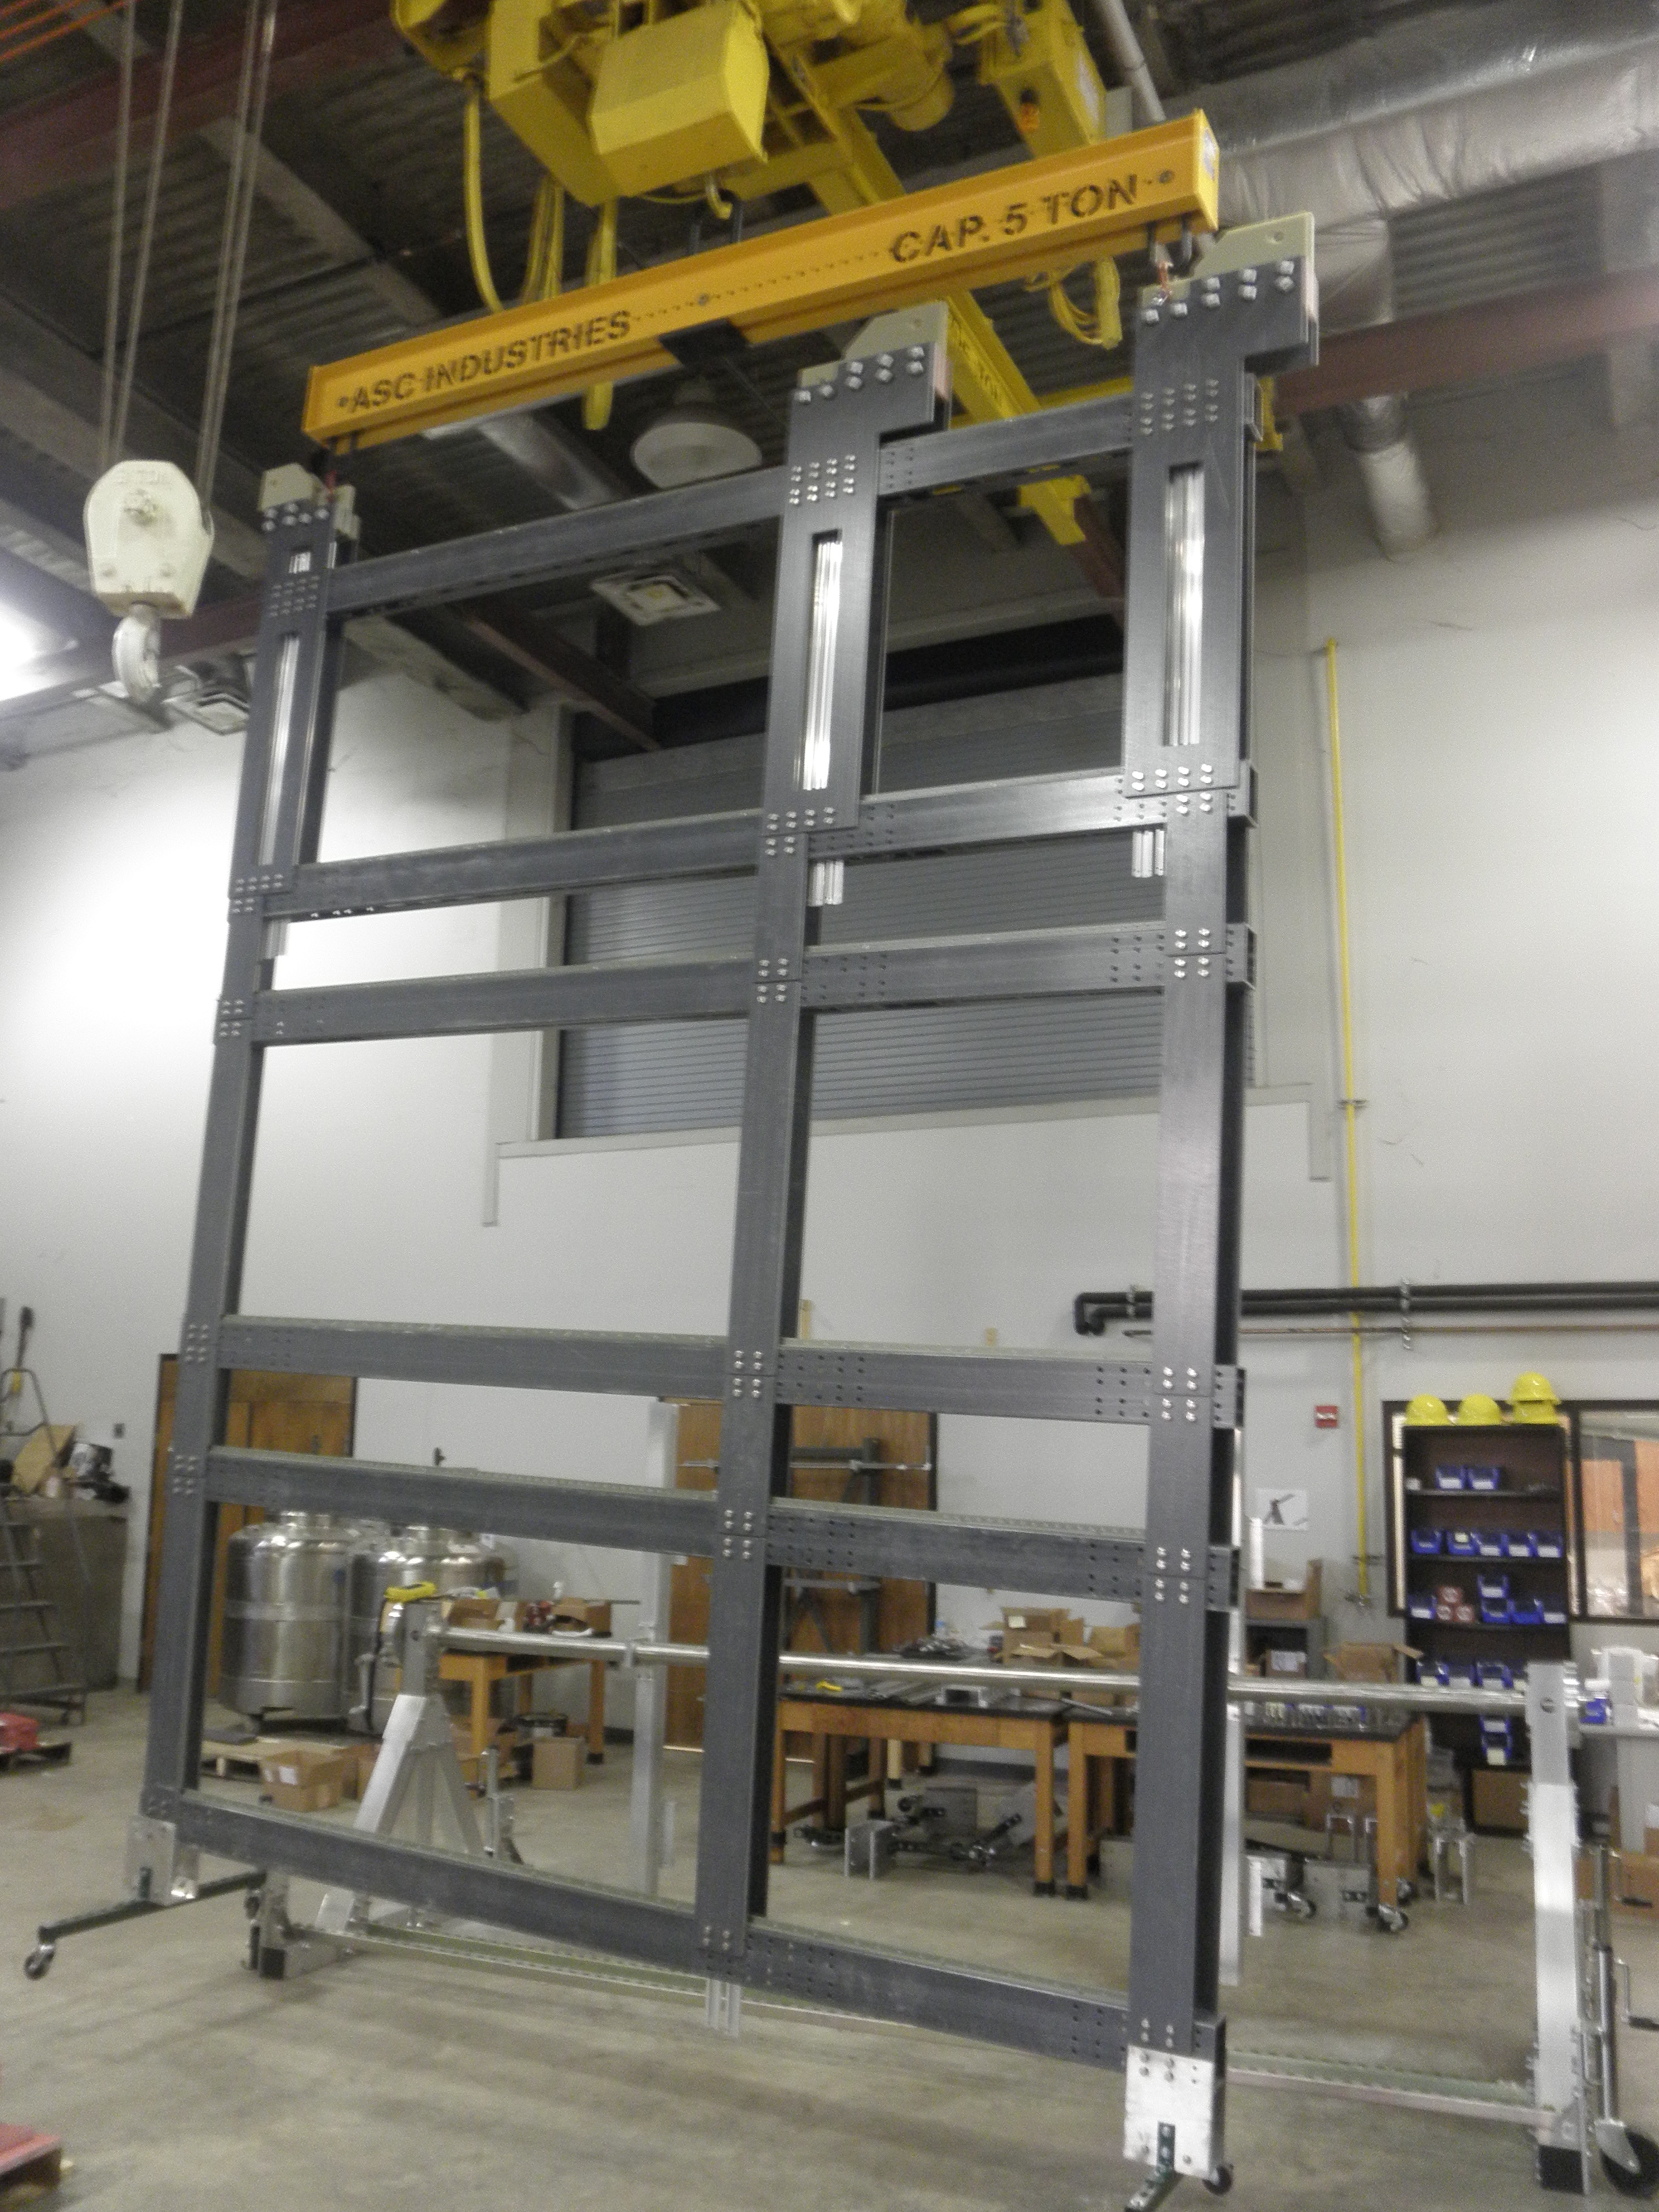
\includegraphics[width=0.5\textwidth]{3_fc_endwall_frames_hanging}
\end{dunefigure}


Aluminum profiles are inserted into the cutouts of the box beams and attached with screws and stainless steel slip nuts to brackets that are mounted on the 
FRP box beams. After this, the resistive divider boards are mounted to the profiles using brass screws that engage with stainless steel slip nuts inside 
the profiles.

%%%%%%%%%%%%%%%%%%%%%%%%%%%%%%%%%%%%
\subsection{Electrical Interconnections}
\label{sec:fdsp-hv-prod-interconnect}

All electrical fasteners and wires used on the \dword{cpa} and \dword{fc} are produced
to specification by commercial vendors and packaged with the \dword{cpa} or \dword{fc} modules.  
As discussed above (\ref{sec:fdsp-hv-prod-cpa}, \ref{sec:fdsp-hv-prod-fc}), 
this includes the \dword{hv} cable segments, as well as wire jumpers, machined brass
tabs, etc.

Circuit boards for %DUNE 
\dword{hv} interconnections are produced and tested at the  university shops according to the same design used for \dword{pdsp}.  The \dword{fc} voltage dividers were produced for \dword{pdsp} at Louisiana State University, and the boards for \dword{cpa} frame bias and \dword{cpa}-\dword{fc} connections were produced at Kansas State University.
%\todo{What about the \dword{fc}-to-\dword{apa} boards?} 
Both institutions have created custom test apparatus for verifying proper operation of the boards at full voltage and over-voltage conditions.  Production and testing could be scaled up by the required order of magnitude at these institutions, or shared with other institutions, whichever best meets the needs of the project. Each board is free of solder flux and flux-remover. 
 
%%%%%%%%%%%%%%%%%%%%%%%%%%%%%%%%%%%%%%%%%%%%%%%%%%%%%%%%%%%%%%%%%%%%
\section{Installation, Integration and Commissioning}
\label{sec:fdsp-hv-install}

%%%%%%%%%%%%%%%%%%%%%%%%%%%%%%%%%%%%
\subsection{Transport and Handling}
\label{sec:fdsp-hv-install-transport}

The power supply, cables, filters, and feedthroughs are sent to the site in standard shipping crates.  Handlers wear gloves when handling insulators that are between \dword{hv} and ground.  Surfaces can be cleaned with alcohol and allowed to dry.

\dword{cpa} panels are shipped in crates to the \surf site.  The \SI{12}{\m} \dword{cpa} panels are disassembled into their three \dword{cpa} units, loaded into the crates with all hardware needed to complete the \dword{cpa} panel assembly at the \surf site.  Each shipment should consist of two crates which contain the two \dword{cpa} panels that will be paired to form a \dword{cpa} plane. There will be very little room for storage at the \surf site, so it is important to ship \dword{cpa} panels in this way so that final assembly, integration, and installation can proceed as soon as components are received.

\Dword{topfc} and \dword{botfc} modules will either be fully assembled at university production sites and shipped to SURF ready for installation into the mine, or the components will fabricated and \dword{qc} inspected at university sites before being shipped to \surf for final assembly, as was done for the \dword{pdsp} modules at CERN. Crate design for \dword{topfc} and \dword{botfc} modules will depend strongly on whether the \dwords{gp} remain attached to the modules, as in the \dword{pdsp} design, or if the \dwords{gp} are, instead, connected directly to the cryostat. In the former case, if fully assembled \dwords{topfc} and \dwords{botfc} modules with attached \dwords{gp} are transported to the underground area, the complexity of the crates is significantly enhanced, as it is difficult to fully support a module on all sides while allowing for tipping of the crate. Hence, it may be necessary for \dwords{gp} to be installed underground in either design scenario. Thus far, only single fully assembled \dwords{topfc} and \dwords{botfc} modules have been crated for shipment, but more complex designs that will allow for multiple modules (without installed ground planes) will be developed.


The \dwords{ewfc} sections each consisting of eight modules are shipped in two separate shipping crates each containing four modules in an upright and vertical orientation.
As was done for ProtoDUNE each \dwords{ewfc} module will be individually wrapped in plastic 
and can be extracted from the crate by means of an overhead crane and spreader bar.
Extracted modules will be rotated into horizontal position using the ledge on a dedicated assembly table. The module side showing steel bolts should be on top for final QC. 


The \dword{hv} bus segments, \dword{fss} bias boards, and  interconnection wires will be integrated with the \dword{cpa} units before shipment, while \dword{cpa} panel interconnections and \dword{fss} connection tabs will be packaged and shipped with the \dword{cpa} panels for integration on site.
\dword{fc} divider boards will be attached to \dword{fc} modules during \dword{fc} assembly as described in \ref{sec:fdsp-hv-prod-fc}.
The \dword{cpa}-to-\dword{fc} and \dword{fc}-to-\dword{apa} boards will be shipped separately and attached just before each \dword{fc} is hoisted onto its \dword{cpa} panel in order to avoid risk of damage to exposed boards on the ends of the \dwords{fc} during shipment and handling.


%%%%%%%%%%%%%%%%%%%%%%%%%%%%%%%%%%%
\subsection{Installation and Integration}
\label{sec:fdsp-hv-integration}
Upon arriving at the SURF site, The \dword{cpa} shipping crate is unpacked with the middle/lower \dword{cpa} unit placed in a vertical stand on the floor of the so-called toaster region, an area in the DUNE detector cavern between the cryostat endwall and the cavern wall set aside for installation functions.  Next, the middle-middle \dword{cpa} unit is removed and vertically attached to the middle-lower Unit.  Finally, the upper-middle \dword{cpa} unit is removed and attached.  This assembly makes up a \dword{cpa} panel.  The \dword{cpa} panel is lifted and vertically attached to its trolley with an FR4 hangar.  Two \dword{cpa} panels are paired to form a \dword{cpa}  plane which then forms the unit for attachment of the \dwords{fc}.  Figure~\ref{fig:cpas-in-cryostat} shows on the left a two-Panel \dword{cpa} plane mounted on its trolleys in the clean room at \dword{pdsp}, waiting for installation of the \dword{topfc} and \dword{botfc} units.

It should also be noted that the \dword{cpa} panels on each end of each \dword{cpa} array are special -- they have aluminum profiles along the exterior side to form the first element of the field cage.  They also contain parts of the \dword{hv} bus mounted on the \dword{cpa} frames.  The \dword{hv} bus forms a continuous loop from the \dword{hv} Input through the top of the 25 \dword{cpa} planes, down the far external side, back along the bottom and up the  external side back to the \dword{hv} Input.

\begin{dunefigure}[\Dword{pdsp} \dword{cpa} plane before and after \dword{fc} attachment]{fig:cpas-in-cryostat}{Left: Completed \dword{pdsp} \dword{cpa} plane ready for \dword{fc} attachment. Right: Two completed \dword{cpa}-\dword{fc} assemblies in the \dword{pdsp} cryostat. The top and bottom \dwords{fc} with their \dwords{gp} attached are visible to the right of the cathode plane in their folded-up pre-installation position.}
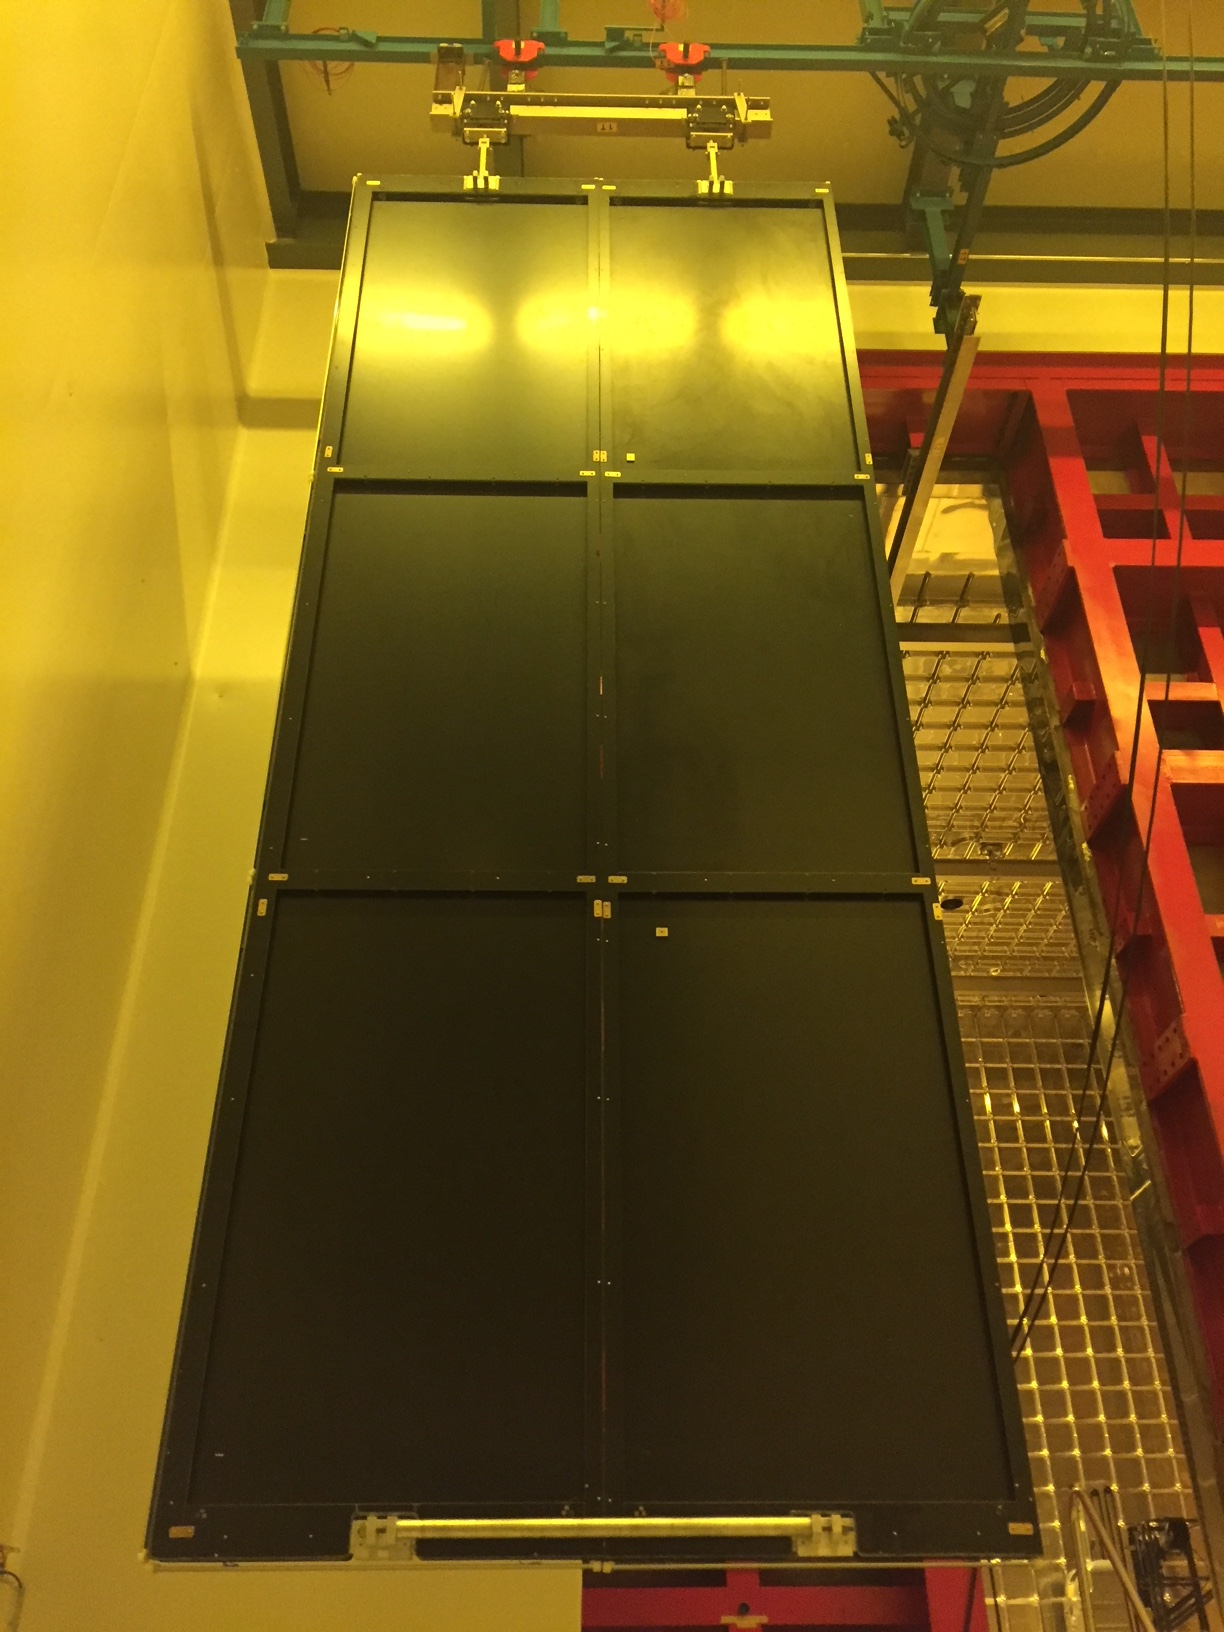
\includegraphics[width=0.45\textwidth]{lastcpa}
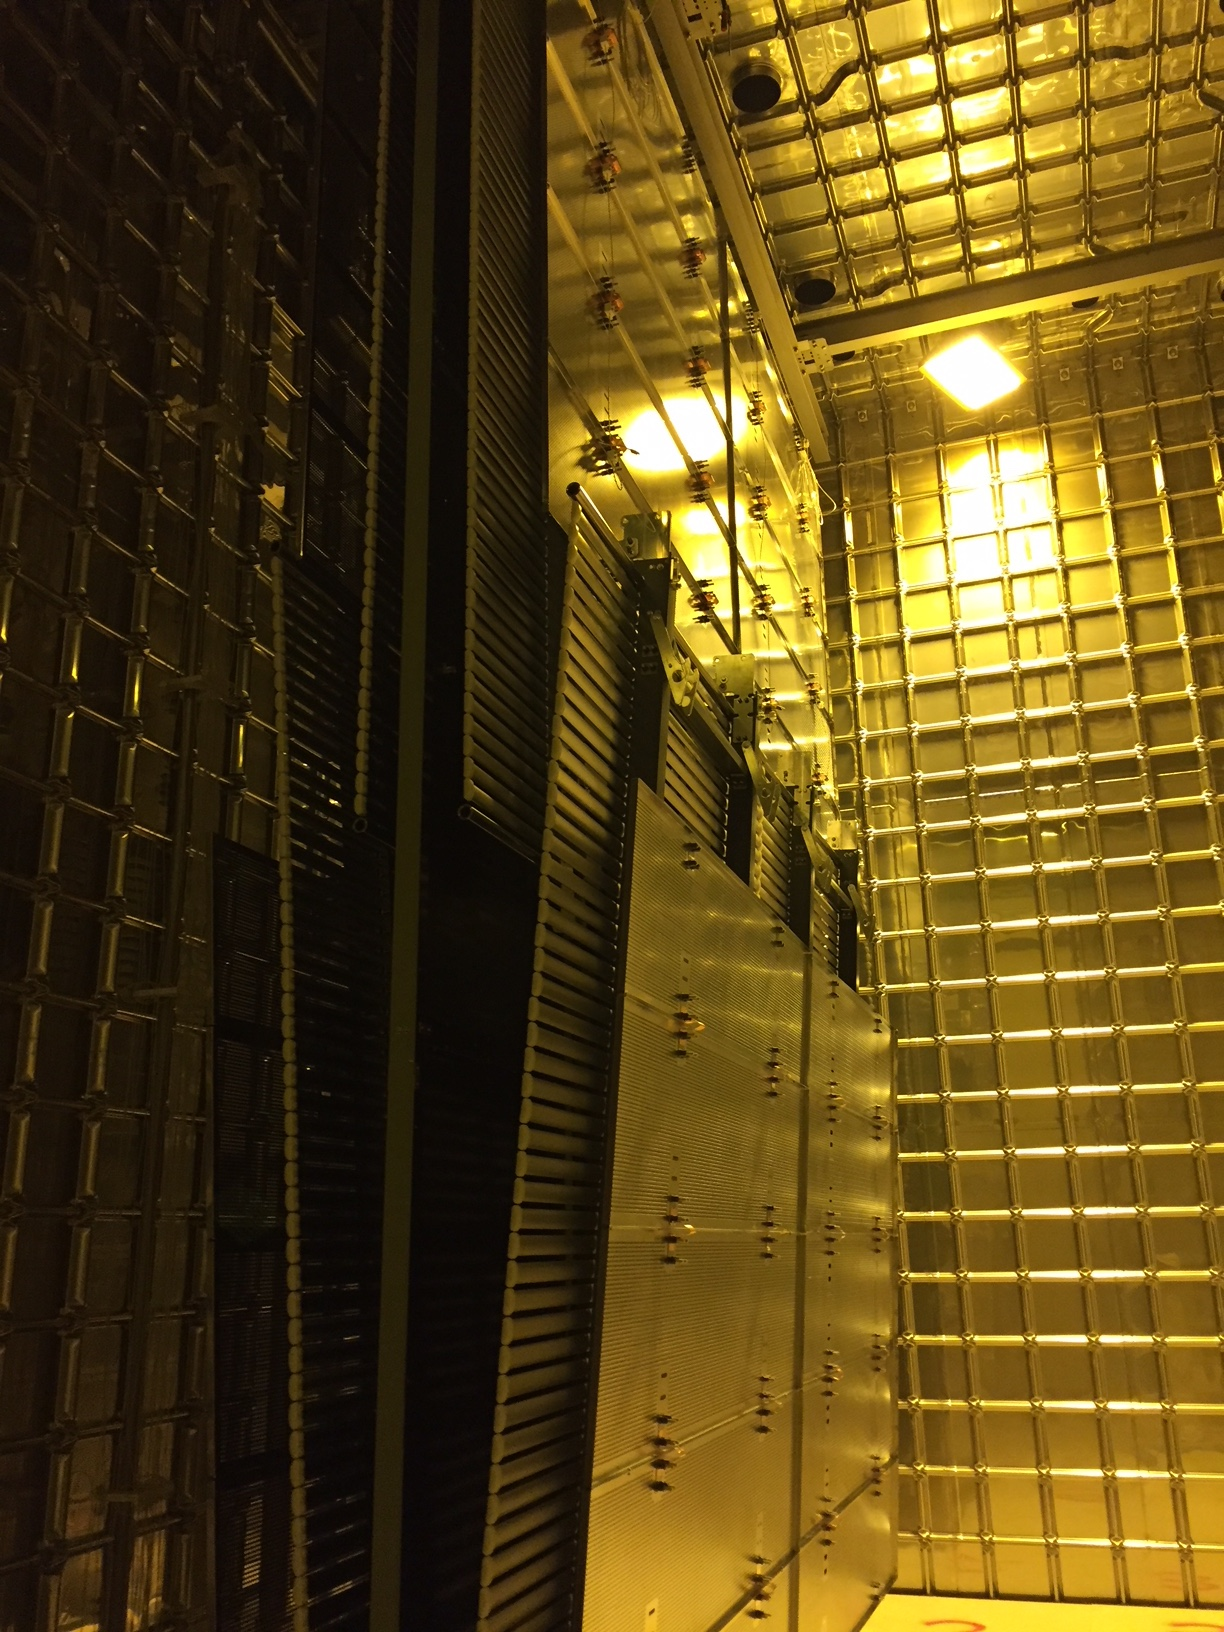
\includegraphics[width=0.45\textwidth]{2cpas-in-cryostat}
\end{dunefigure}

There are a total of 50 \dword{cpa} panel pairs (\dword{cpa} planes) arranged in the %DUNE cryostat 
\dword{spmod} in two rows of 25 each.  After the panels are paired, \dword{fc} units are attached folded against the \dword{cpa} and the full \dword{cpa}-\dword{fc} assembly is placed in the \dword{spmod} cryostat through the access door.  Figure~\ref{fig:cpas-in-cryostat} shows on the right two completed \dword{cpa}-\dword{fc} assemblies on their beam in the \dword{pdsp} cryostat. Upon deployment of the folded top and bottom \dword{fc} units, and after the final \dword{ewfc} installations, the \dword{tpc} \dword{fc} is complete.

To assemble the \dword{ewfc}, the modules are rotated vertically in the assembly area, then placed in a stand designed to hold the \SI{120}{\kg} pieces vertically. The \dword{topfc} is lifted and moved above the next module in the vertical stand where the two are bolted together and any electrical connections are made. The two modules are then lifted up and aligned above the following module.  The modules are again bolted, electrically connected and raised and aligned above the next piece.  This process is repeated until all eight modules are hanging together.  Once the bolting and electrical connections have been completed on the last piece, the continuity of all the grounding connections of the \dword{ewfc} are checked.
 
The completed \dword{ewfc} section is then moved over to the installation beam where its spreader bar is attached to the installation system.  It is then rolled into the cryostat and located on the appropriate beam for installation into the \dword{tpc}.

\begin{dunefigure}[\Dword{pdsp} \dword{ewfc} installation]{fig:EndwallInstall}{Completed endwall in process of installation into \dword{pdsp} cryostat.}
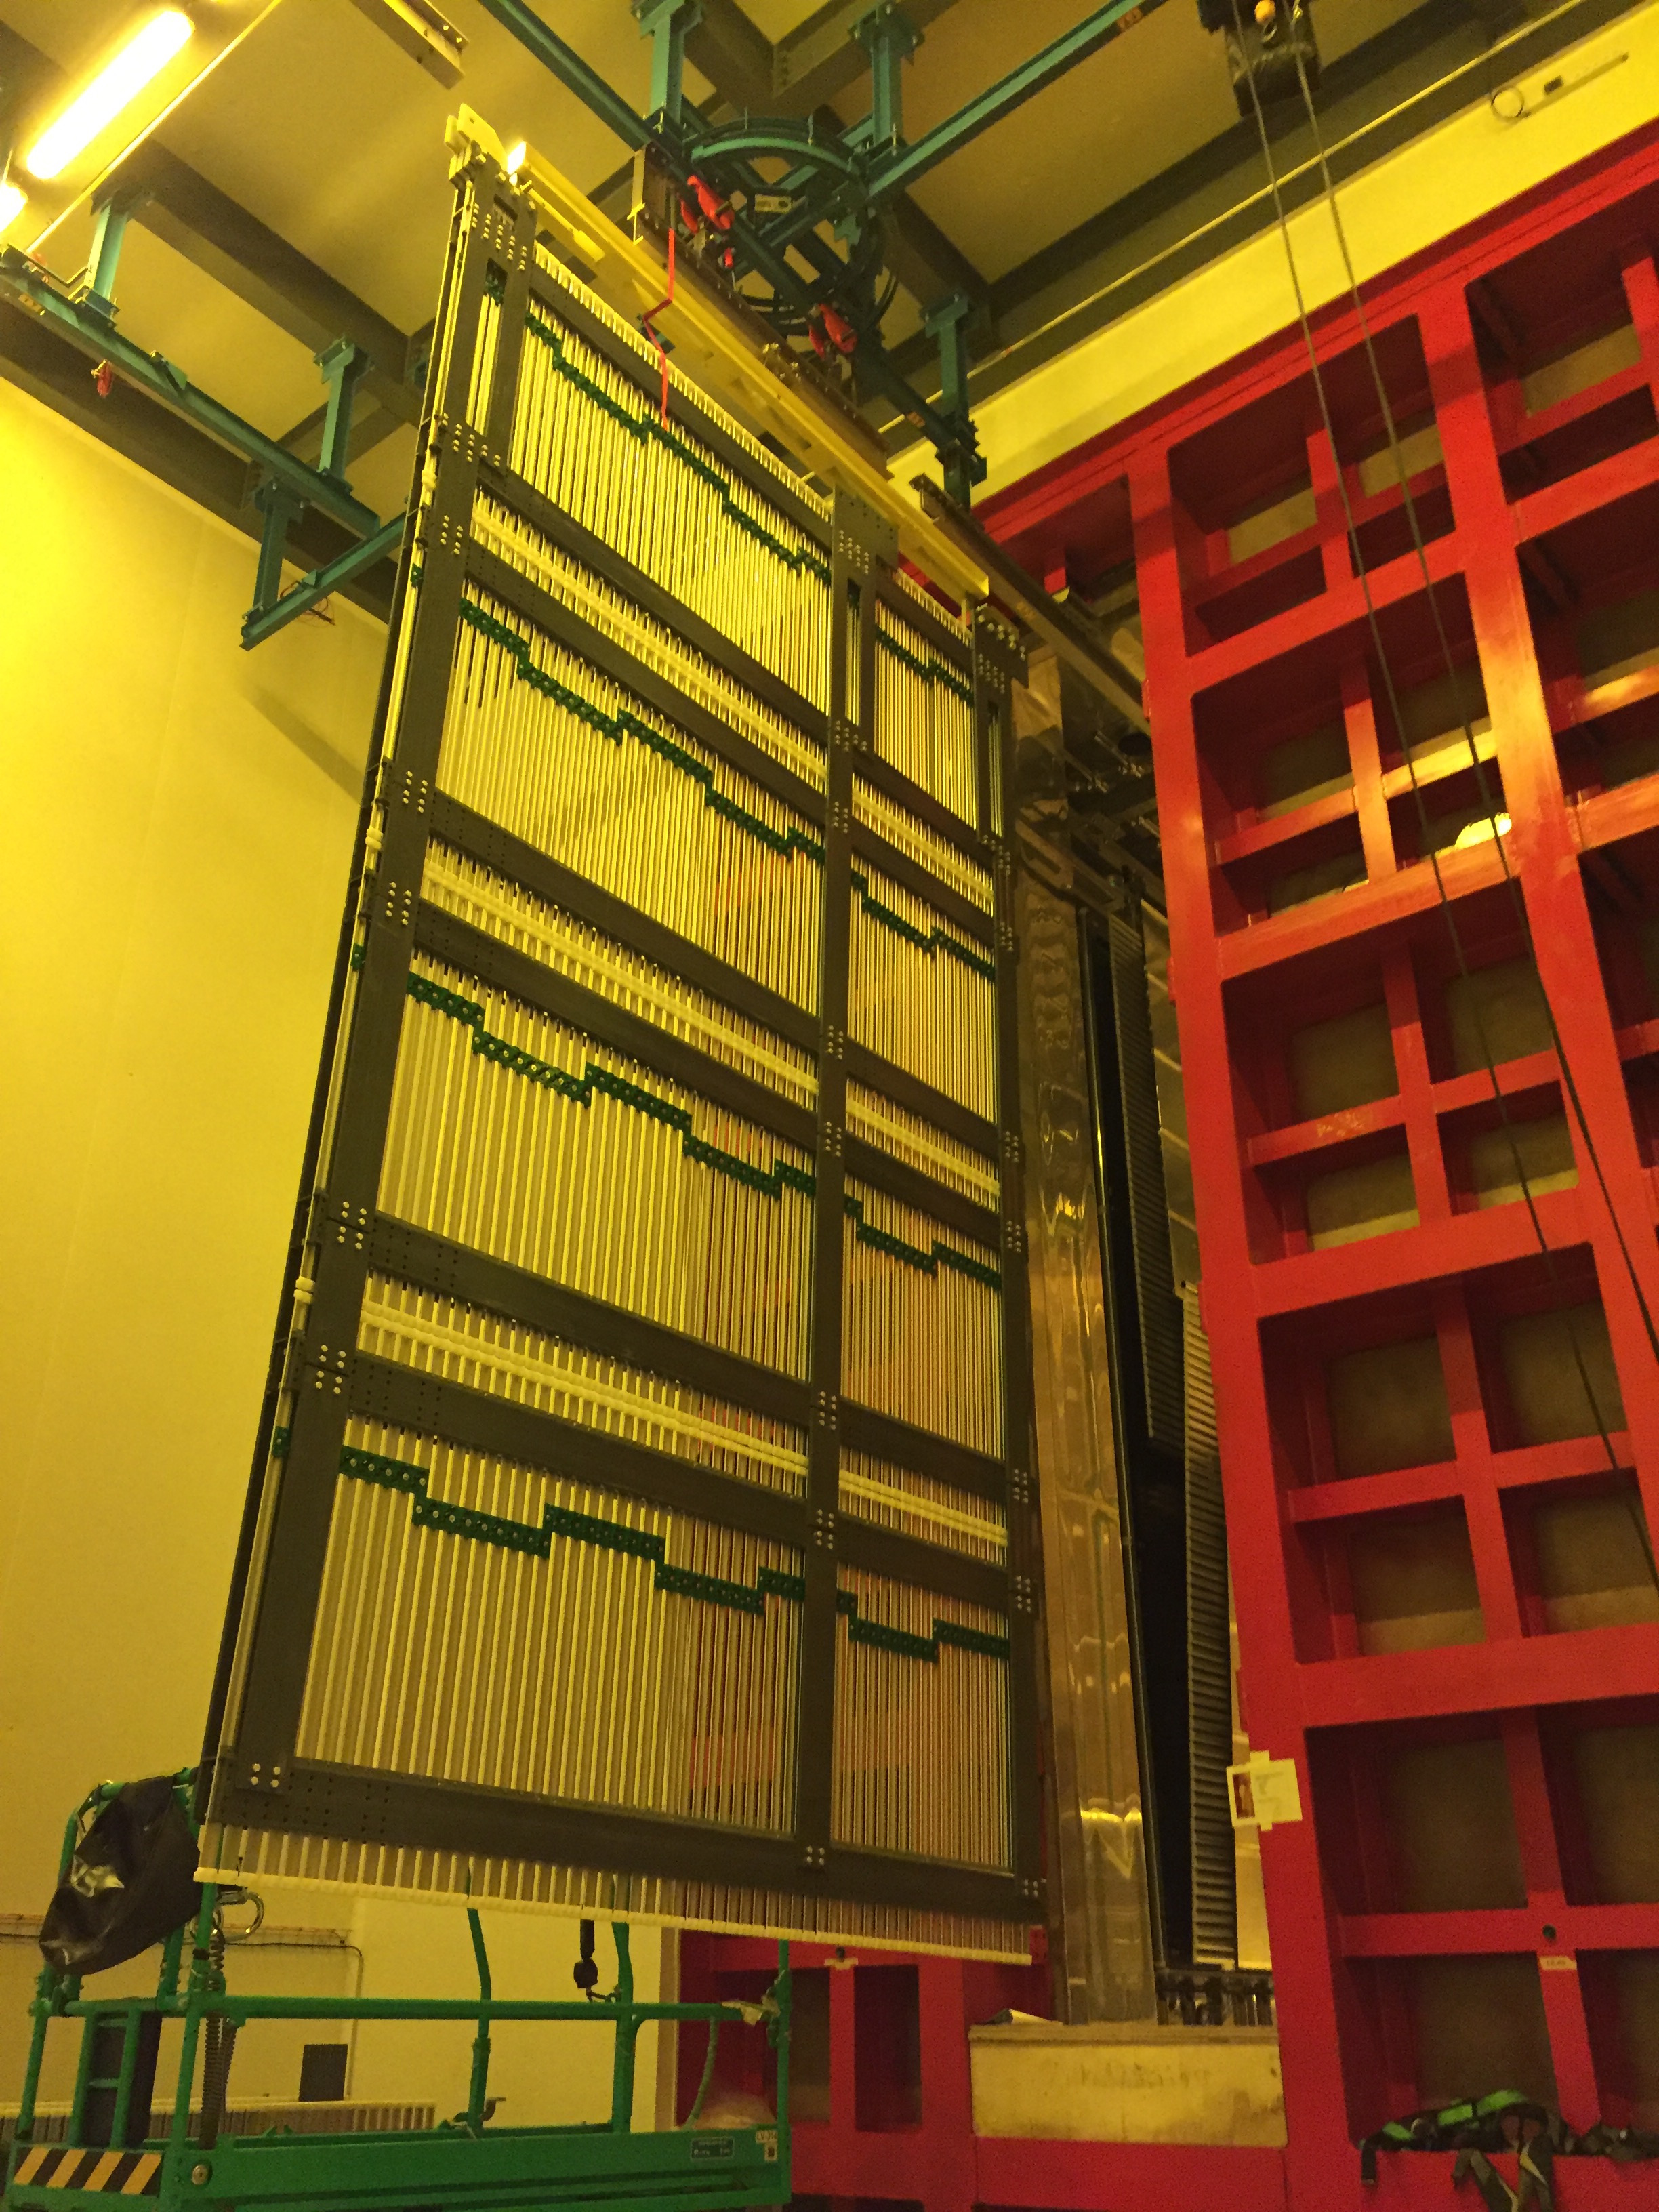
\includegraphics[width=0.45\textwidth]{endwall_and_tco.jpg}
\end{dunefigure}



\subsection{Interfaces}
\label{sec:fdsp-hv-interface}

Among \dword{tpc} components there are internal interfaces between the \dword{cpa} and \dword{fc}; the \dword{cpa} and \dword{hv}, and  the \dword{fc} and \dword{hv}. In addition there are significant interfaces with systems from other consortia.

The interfaces with the \dword{hv} system include the electrical connections with the \dword{hv} cup, \dword{hv} bus, and \dword{fc}, interconnecting the panels within the \dword{cpa}, and propagating the \dword{hv} bus between adjoining \dwords{cpa}.  A selection of the mechanical interfaces are as follows:
\begin{itemize}
\item Metal contact plates on the cathode surface at each corner, with two captive screws in each, used for making electrical contact with the \dword{hv} bus and the resistor board for the frame field strips;
\item Through holes for the \SI{3}{\milli\m} diameter cable in the sides of each frame adjacent to the contact plates to allow interconnection of the \dword{hv} bus between \dwords{cpa};
\item A means of securing the \dword{hv} bus cable in place;
\item Through-holes near the centers of the top and bottom frames for connecting the \dword{topfc} and \dword{botfc} elements to the cathode, with corresponding metal contact plate on the cathode surface;
%\item Electrical specifications for these parts and interfaces are given in the \dword{hv} design Section 
\item Between the \dword{cpa} and the \dword{fc} the interface at the hinge joint ensures that the \dword{cpa} and \dword{fc} are properly located relative to each other.
\end{itemize}
%\fixme{last bullet: hinge joint that ensures...?}
Since these interfaces occur within the design group that is constructing the \dword{tpc} there is close coordination and communication between the \dword{cpa}, \dword{fc} and \dword{hv} groups to ensure that all requirements are met and that the components all fit together.

The interfaces between the \dword{cpa} system and the \dword{hv} system, and the interfaces among the \dword{cpa}-\dword{fc}-\dword{hv} systems are shown in integration drawings and documented in the project documentation system. \fixme{reference properly. RKP: Requires reference policy, under discussion.}

%DUNE-3 is a drawing that is used to define the interface between the \dword{cpa} system and \dword{hv} system and DUNE-6 is an integration drawing that defines the interface between the \dword{cpa}/\dword{fc}/\dword{hv} systems.  These drawings can be found in DocDb 1870. 

The various components in the \dword{hv} system also have interfaces with components from other systems.  These interfaces are formally defined by interface documents. 
 %Detailed descriptions of major interfaces in DUNE can be found (here?). 
 
Key interfaces between the \dword{hv} and other systems are summarized in Table~{\ref{tab:hvinterfaces}}.

%The external interfaces and defining DOCDB number are listed in the table below.


%Interface	DOCDB 
%\dword{tpc} with Cryostat	1677
%\dword{tpc} with Detector Support Structure	1681
%\dword{tpc} with Photon Detection System	1682
%\dword{tpc} with DAQ/Computing/Slow Controls	1683
%\dword{tpc} with Rack Space and Power Requirements	1684



\begin{dunetable}
[\dword{hv} system interfaces]
{p{0.2\linewidth}p{0.75\linewidth}}
{tab:hvinterfaces}
{Key \dword{hv} System Interfaces to Other Systems} 
Interface to & Description \\ \toprowrule
DSS  &  Support, positioning, and alignment of all \dword{cpa}, \dword{fc} modules inside the cryostat both warm and cold\\ \colhline
\dword{apa} & \dword{fc} support (top, bottom, and end wall) on \dword{apa} frames; Mounting of field cage termination filter boards and \dword{fc} failsafe terminations; Mounting of the electron diverter boards.
\\ \colhline
\dword{tpc} Elec. & \dword{fc} termination wire connectors on CE feedthrough flange, \dword{fc} termination wires routed with CE cables
 \\ \colhline
PDS & Mounting of PD calibration flash diffusers and routing of their fibers to \dwords{cpa}; Possible \dword{tpc} coated reflector foil on \dword{cpa}s.
 \\ \colhline
Facility & Locations and specifications of the \dword{hv} Feedthrough ports; gas and \dword{lar} flow velocities and patterns. \\ \colhline
Calibration & \dword{fc} openings for the calibration laser heads \\ \colhline
Cryogenic Instrumentation \& Slow Control. & \dword{hv} vs. \dword{lar} level interlock, sensor locations in high field regions, cold/warm camera coverage, \dword{hv} signal monitoring, etc. 
 \\ \colhline
Integration Facility & Storage buffer, inspections/tests, repackage for underground delivery
 \\ \colhline
Physics / Software & Requirements: range of operating drift field, uniformity of the drift field; Supply detector geometry and \efield{} map.
 \\ 
\end{dunetable}

%%%%%%%%%%%%%%%%%%%%%%%%%%%%%%%%%%%%%%%%%%%%%%%%%%%%%%%%%%%%%%%%%%%%
\section{Quality Control (QC)}
\label{sec:fdsp-hv-qc}

Power supplies used in a \dword{spmod} will be tested before installation.  Output voltages and currents must be checked on a known load. 

The feedthrough and filters should be tested at the same time, preferably with the planned power supply.  The feedthrough must be tested to hold the required voltage in \dword{tpc}-quality \dword{lar} ($\tau\geq$\SI{1.6}{ms}) for several days.  The ground tube submersion and \efield{} environment of the test setup should be comparable to the real field cage setup or more challenging (e.g., the test liquid level can be lower than %DUNE's 
that in the \dword{spmod} but not higher).  Additionally, the feedthrough must be leak-tight to satisfy cryogenics requirements.

\Dword{cpa} \dword{qc} consists of forms that are filled out as part of the various procedures from initial assembly at factories to the final testing of connections in the DUNE cryostat.  A group of \dword{qc} forms filled out during initial panel unit assembly travels in the shipping crate with the panel.  At SURF, \dword{cpa} panel and \dword{cpa} plane assemblies have their own set of \dword{qc} forms for \dword{cpa} assembly and for \dword{cpa}-\dword{fc} integration.  Finally, before top and bottom \dword{fc} deployment, a final check of all electrical connections on the \dword{cpa} and between the \dword{cpa} and the top, bottom, and endwall \dwords{fc} is completed.  

Before assembly and shipment of \dword{topfc} and \dword{botfc}, each FRP component is subjected to inspection.
%prior to assembly.
Each of the beams is checked for flatness, torsion, and structural and surface defects, such as cracks or fractures, layer separation, thermal decomposition, and evidence of water-induced bloating. Any scratching or grooving of the surface layer can be remediated by coating with commercially available epoxy.

%%%%%%%%%%%%%%%%%%%%%%%%%%%%%%%%%%%%
%\subsection{During Local Production and Assembly}
%\label{sec:fdsp-hv-qc-local}

%QC Local for Endwalls
For the \dwords{ewfc}, each box beam and all FRP stock will be inspected prior to assembly for dimensions, deformations, surface scratches and delamination defects. If the inspection is not passed, the parts will be rejected.
Preliminary assembly of \dwords{ewfc} modules will take place in a high-bay area under full crane access. After assembly, individual \dwords{ewfc} modules will be hung off each other in pairs of two to test the interconnections of the modules. Hanging will be performed in a top-down sequence consistent with space constraints (maximum three at once). This process will be repeated for all \dwords{ewfc}. All parts will be labeled to uniquely identify their position. After disassembly, all parts are cleaned before being moved into the clean room, where they will be inspected again. Final assembly will occur in a dedicated clean laboratory space.

Each panel will undergo mechanical and quality control tests  before shipping. 
\fixme{lsu - do we want to specify?} Electrical \dword{qc} tests will be performed after assembly of all aluminum profiles and resistor divider chains and again prior to installation of the \dwords{ewfc} into the cryostat. These tests will be performed with a pico-ammeter to measure the nominal resistance between profiles while grounding neighboring profiles not involved in any particular measurement.


%%%%%%%%%%%%%%%%%%%%%%%%%%%%%%%%%%%
%\subsection{Post-factory Installation (Remote)}
%\label{sec:fdsp-hv-qc-remote}

%QC remote for Endwalls
Once at SURF, all \dwords{ewfc} panels shall be inspected visually after unpacking and prior to installation. Electrical tests will be repeated at various stages of the staging and installation process.
The tests will be again be performed with a pico-ammeter to measure the nominal resistance between profiles while grounding neighboring profiles.

% QC local for interconnections
During electrical interconnections local assembly, quality control inspection checklists for \dword{cpa}, \dword{fc}, and
interconnections will be adapted from \dword{pdsp} checklists for \dword{cpa}
panels, \dword{hv} bus segments, interconnection wires, and resistor boards.
These checklists include physical inspection for defects and
resistance tests.  For maximum traceability, checklists may be both
filed in an electronic logbook and sent in hard copy along with the
components tested.

% QC remote for interconnections
For the electrical interconnections \dword{qc} at SURF, expected resistances have been modeled at all stages of
\dword{cpa}+\dword{fc} integration.  The height of the \dwords{cpa} make it best to catch a
faulty connection as early as possible.  This will be achieved by
quickly checking resistances for expected values between \dword{cpa} panels and between \dword{cpa} panels and field strips as \dword{cpa} unit subassemblies are added.  Profile-to-profile field cage resistances
will be checked upon reception and rechecked immediately before
attaching to \dwords{cpa} underground.  Once all four \dwords{fc} are attached to a
\dword{cpa}, resistances between selected \dword{fc} profiles and the \dword{hv} bus will be
measured, checked against expected values, and recorded. Continuity of
the \dword{hv} bus between \dwords{cpa} will be checked at top and bottom as each \dword{cpa}
is connected to its neighbor inside the cryostat.


%%%%%%%%%%%%%%%%%%%%%%%%%%%%%%%%%%%%%%%%%%%%%%%%%%%%%%%%%%%%%%%%%%%%
\section{Safety}
\label{sec:fdsp-hv-safety}

Safety is central to the design of the \dword{hv} system. In all phases including fabrication, installation, and operations, safety will be the highest priority. There will be documented assembly, testing, transport, and installation procedures. Particular attention was paid to these topics in the design of  
\dword{pdsp}  with explicit concern to a design that is identical to the \dword{spmod} design, the most critical of which are also noted in the preliminary \dword{hv} risk assessment, which is under development. %\fixme{ref properly. RKP: Requires reference policy, under discussion.}

The structural and electrical designs for the \dword{sp} \dword{hv} are based on designs that were vetted and validated in the \dword{pdsp} construction, which is currently in its final phase of deployment at CERN. Previously, Fermilab \dword{hv} tests implemented a full-voltage and full-scale \dword{hv} feedthrough, power supply, filtering, and monitoring system, along with the \dword{hv} connection cup and arm, after completing full safety reviews. These devices worked as designed and are essentially reproduced in both \dword{pdsp} and the \dword{spmod}. 

When operating the \dword{fc} at its full operating voltage there is a substantial amount of stored energy. The design of the \dword{cpa} is centered around storing charge  at the highest voltage on a resistive surfaces to limit the power dissipated during a power supply trip or other failure which unexpectedly drops the \dword{hv}. This design has been successfully tested at full voltage over \num{2}\,m$^2$ surfaces at full voltage and will soon be tested at larger scale in \dword{pdsp}.  

Integral to the \dword{sp} \dword{fc} design, both in \dword{pdsp} and the \dword{spmod}, is the concept of pre-assembled modular panels of field-shaping conductors with individual voltage divider boards. The structural design and installation procedures used in \dword{pdsp} were selected to be compatible with use at the Far Detector site and were vetted by project engineers, engineering design review teams, and CERN's safety engineers. Some revisions to these designs are expected based on lessons learned in installation and operations; these revisions will be reviewed both within the Project and by Fermilab \dword{esh} personnel. The overall design is on solid footing. 

Assembly of the \dword{fc} panels and resistor-divider boards will involve collaboration technical, scientific, and student labor and  does not present unusual industrial hazards. The \dword{hv} consortium will work closely with each assembly site to ensure that procedures meet both Fermilab and institutional requirements for safe procedures, personal protective equipment, environmental protection, trained materials handling, and training. The vast majority of production part fabrication will be carried out commercially and shipping will be contracted through approved commercial shipping companies. Prior to approving a site as a production venue, each site will be visited and reviewed by an external safety panel to ensure best practices are in place and maintained. 

%% B. Yu: this following paragraph should be reserved for the DP chapter    
%
% The DP \dword{hv} power supply and \dword{hv} delivery system design is more challenging due to the required 600kV power supply needed to provide field across the 12m drift volume. A half-voltage system will be used in the 6m drift volume in the ProtoDUNE-DP, and is based on similar experiences to the SP \dword{hv} tests. The supply is expected to be a custom supply from an experienced vendor, and is currently envisioned as being secured from the same vendor who is providing the ProtoDUNE and Far Detector SP supplies. Similar power dissipation management considerations are being investigated in the DP design, but are somewhat less advanced that the SP field cage design and will require addition R\&D and engineering to be finalized. 

%%%%%%%%%%%%%%%%%%%%%%%%%%%%%%%%%%%
% add subsections and labels if needed \subsection{}
%\label{sec:fdsp-hv-safety-}


%%%%%%%%%%%%%%%%%%%%%%%%%%%%%%%%%%
%\subsection{}
%\label{sec:fdsp-hv-safety}



%%%%%%%%%%%%%%%%%%%%%%%%%%%%%%%%%%%%%%%%%%%%%%%%%%%%%%%%%%%%%%%%%%%%
\section{Organization and Management}
\label{sec:fdsp-hv-org}


%%%%%%%%%%%%%%%%%%%%%%%%%%%%%%%%%%%
\subsection{HV System Consortium Organization}
\label{sec:fdsp-hv-org-consortium}

The consortium consolidates all the institutions that are participating in the design, construction and assembly of the \dword{hv} systems for both \dword{pdsp}  and \dword{pddp}. It is currently composed of US institutions and CERN, presently the only non-USA participant. As in the case of \dword{protodune}, CERN is heavily committed to a significant role in terms of funding, personnel, 
 and the provision of infrastructure for R\&D and detector optimization. Moreover, CERN will be responsible for a significant fraction of subsystem deliverables; as such it is the intention of CERN to attract additional European institutions into the consortium.


%There is still a need to expand this list in the near future by an effort to include new EU participants.



\begin{dunetable}
[\dword{hv} consortium participants]
{p{0.35\linewidth}p{0.25\linewidth}p{0.35\linewidth}}
{tab:hvconsortiumparticipants}
{\dword{hv} Consortium Participants as of May 2018}   
 Institution & Investigator & Contact \\ \toprowrule
EU: CERN & Francesco Pietropaolo & francesco.pietropaolo@cern.ch  \\ \colhline
USA: Argonne National Lab   &   Steve Magill   &   srm@anl.gov   \\ \colhline
USA: Brookhaven National Lab  &  Bo Yu  &  yubo@bnl.gov  \\ \colhline
USA: University of California (Berkeley)  & Cheng Ju Lin  &  cjslin@lbl.gov  \\ \colhline
USA: University of California (Davis)  & Emilija Pantic   &   pantic@ucdavis.edu  \\ \colhline
USA: Fermi National Accelerator Lab  & Sarah Lockwitz   &   lockwitz@fnal.gov  \\ \colhline
USA: University of Houston & A. Renshaw   &   arenshaw@central.uh.edu  \\ \colhline
USA: Kansas State University & Glenn Horton-Smith   &   gahs@ksu.edu  \\ \colhline
USA: Lawrence Berkeley National Lab & Cheng Ju Lin   &   cjslin@lbl.gov  \\ \colhline
USA: Louisiana State University & Thomas Kutter   &   kutter@phys.lsu.edu  \\ \colhline
USA: South Dakota School of Mines and Technology  & J. Reichenbacher	&   Juergen.Reichenbacher@sdsmt.edu  \\ \colhline
USA: Stony Brook University  & Micheal Wilking   &   michael.wilking@stonybrook.edu  \\ \colhline
USA: University of Texas (Arlington) & Jaehoon Yu   &   jaehoonyu1@gmail.com  \\ \colhline
USA: Virginia Tech. & Jon Link   &   jmlink@vt.edu  \\ \colhline
USA: William and Mary  &  Jeff Nelson   &   jknels@wm.edu  \\
\end{dunetable}

The Consortium has the following Management Structure:
\begin{itemize}
 \item Consortium Leader: Francesco Pietropaolo (CERN)
 \item Technical Leader: Bo Yu (BNL)
 \item TDR/TP Editor: Rob Plunkett (FNAL)
 \item \dword{hv}S design and integration lead: Vic Guarino (ANL)
\end{itemize}

In the \dword{hv} consortium organization, each institution is naturally assuming the same responsibilities as for the developments of \dword{pdsp}. The consortium is organized into working groups addressing the design and  R\&D phases and the hardware production and installation.

\begin{itemize}
\item WG1. Design optimization for \dword{spmod} and \dword{dpmod}; assembly, system integration, detector simulation, physics requirements for monitoring and calibrations. Conveners: Jeff Nelson, Vic Guarino, Bo Yu
\item WG2. R\&D activities, R\&D facilities. Conveners: Francesco Pietropaolo, Ting Miao
\item WG3. \dword{sp}-\dword{cpa}: Procurement, in situ \dword{qc}, resistive panels, frame strips, electrical connections of planes; \dword{qc}, assembly, shipment to assembly site; \dword{qc}. Convener: Stephen Magill
\item WG4. \dword{dp} cathode. Convener: Jae Yu
\item WG5. \dword{fc} modules. Conveners: Thomas Kutter, Michael Wilking, Jeff Nelson, Jae Yu
\item WG6. \dword{hv} supply and filtering, \dword{hv} power supply and cable procurement, R\&D tests, filtering and receptacle design and tests. Conveners: Franco Sergiampietri, Sarah Lockwitz
\end{itemize}

\noindent Merging of \dword{sp} and \dword{dp} groups is envisaged for the working groups where synergies are being identified: \dword{hv} feedthroughs, voltage dividers, aluminum profiles, FRP beams, and assembly infrastructure.

%%%%%%%%%%%%%%%%%%%%%%%%%%%%%%%%%%
\subsection{Planning Assumptions}
\label{sec:fdsp-hv-org-assmp}
The present baseline design for all elements of the \dword{spmod} (\dword{cpa}, top/bottom \dword{topfc}, \dword{botfc}, \dword{ewfc} and \dword{hv} distribution) follows the \dword{pdsp} design as it has been produced and is being assembled.  It is also assumed that no major issues in the \dword{hv} operation of \dword{pdsp} will be encountered and therefore that the basic \dword{hv} concepts are sound.

However some design modifications/simplifications are envisaged to be implemented to take into account the different height of the \dword{cpa}  and the \dword{ewfc} modules and to adapt the installation procedure to the underground environment.

Additional design modifications could be expected if the \dword{pdsp} test run (as well as tests at Fermilab using the \SI{35}{\tonne} cryostat) identifies weaknesses in the present baseline option.

%Similar considerations hold for the DP Field Cage, which will be an extended replica of the ProtoDUNE DP case. The DP \dword{hv} System distribution and the related cathode structure will require instead intense R and D, given the unprecedented value of the required \dword{hv} (-600 KV). 

\dword{pdsp} is the testbed to understand and optimize detector element assembly, installation sequence, integration as well as requirements in manpower, space and tooling, and schedule. 

%%%%%%%%%%%%%%%%%%%%%%%%%%%%%%%%%%%

%\fixme{The editors at meeting of 2/13 suggest that the WBS section should be deleted in the TP. Accordingly, I have commented it out. RKP}

%%%%%%%%%%%%%%%%%%%%%%%%%%%%%%%%%%%
%\subsection{WBS and Responsibilities}
%\label{sec:fdsp-hv-org-wbs}
%
%Consortium deliverables and related Working Breakdown Structure have also been derived from those identified for the ProtoDUNE detectors. As already mentioned before, responsibilities have been assigned to the institutions members of the Consortium, according to the experience gained with ProtoDUNE.
%
%\fixme{(Here: table to be extracted for the WBS excel file)}
%
%%%%%%%%%%%%%%%%%%%%%%%%%%%%%%%%%%
\subsection{High-level Cost and Schedule}
\label{sec:fdsp-hv-org-cs}

%A first high-level summary of the cost estimate for the \dword{hv} system of one \dword{spmod} has been obtained extrapolating from the as-realized \dword{pdsp} costs and and effort. These estimates do not include any projected cost savings that would be realized by producing many units at each production site. Given the small numbers of each unit required for the \dword{pdsp} (e.g., 12 \dword{topfc} and \dword{botfc} modules and 16 \dword{ewfc} modules) the assembly sites were still climbing the learning curve; this could give substantial savings. 

%\begin{dunetable}
%[\dword{hv} system materials costs]
%end{dunetable}

%\begin{dunetable}
%[HV system construction effort by job class]
%\end{dunetable}

\begin{dunetable}
[\dword{hv} system R\&D program and milestones to lead to CD-2 approval]
{p{0.07\linewidth}p{0.55\linewidth}p{0.10\linewidth}p{0.10\linewidth}p{0.10\linewidth}}
{tab:HVschedule}
{DRAFT- \dword{hv} system R\&D program and Milestones to lead to CD-2 approval.}   
WBS&Task Name&Start&Finish \\ \toprowrule
%1&DUNE Milestones&394&4/2/18&10/4/19 \\
%1.4&   Submission of DUNE Technical Design Report (TDR)&
% 4/1/19&
%4/1/19 \\
1.5& CD-2 DOE Review& 10/4/19& 10/4/19 \\ \colhline
7& \dword{hv} system& & \\ \colhline
7.1& Finalize \single \dword{fc} design& 06/27/18& 09/30/19 \\ \colhline
7.2& Finalize \single cathode design& 06/27/18& 09/30/19 \\
7.3& Run \dword{sp} \dword{hv} design integration test& 01/01/18& 12/31/19 \\ \colhline
7.4& \dword{hv} \dshort{tdr} - submit for internal review& 03/29/19& 03/29/19 \\ \colhline
7.5& \dword{cpa} procurement& 09/21/21& 12/06/22\\ \colhline
7.6& \dlong{gp} procurement& 08/08/22& 12/06/22\\ \colhline
7.7& Assemble and test voltage dividers& 08/08/22& 12/06/22\\ \colhline
7.8& \dword{fc}  procurement&  03/11/22& 12/06/22\\ \colhline
7.9& Production readiness reviews& 01/02/23& 01/07/23\\ \colhline
7.10& Cryostat  ready for TPC installation& 05/01/23& 05/01/23 \\ \colhline
7.11& \dword{cpa} assembly& 01/31/23& 07/25/23\\ \colhline
7.12& Top-bottom \dword{fc} assembly&01/31/23& 07/25/23\\ \colhline
7.13& \Dword{ewfc} assembly & 01/05/23& 04/23/23\\
\end{dunetable}
